\documentclass[a4paper,pdftex,12pt]{report}

\usepackage[spanish]{babel}
\usepackage[T1]{fontenc}
\usepackage[latin1]{inputenc}
\usepackage{lmodern,textcomp}
\usepackage[pdftex]{graphicx}
\usepackage[margin=2cm]{geometry}
\usepackage{url}
\usepackage{pdflscape}
\usepackage{multirow}
\usepackage[pdftex]{hyperref}

\hypersetup{
  colorlinks=true,
  bookmarks,
  % citecolor=black,
  % filecolor=black,
  % linkcolor=black,
  % urlcolor=black,
  pdfauthor={Sebasti�n M�nera �lvarez},
  pdftitle={Documentaci�n de HORUS},
  pdfkeywords={monitorizaci�n costera, HORUS},
  pdfsubject={Documentaci�n de HORUS}
}

\addto\captionsspanish{%
  \renewcommand{\contentsname}%
    {Contenido}%
  \renewcommand{\listfigurename}%
    {Lista de Figuras}%
  \renewcommand{\listtablename}%
    {Lista de Tablas}%
}



\begin{document}
%\maketitle

\begin{titlepage}
  \large
  \null\vfill
  
  \begin{center}

    {\huge \textbf{SISTEMA DE MONITORIZACI�N} \\[0.1cm]
      \textbf{AMBIENTAL BASADO EN VIDEO:}\\[0.3cm]
      \textbf{HORUS}}

    \vskip 2cm

    \begin{minipage}[htbp]{1.0\linewidth}
    \begin{center}
      \textbf{Director}:\\
      Andr�s Fernando Osorio Arias, Ph.D.\\
      \href{mailto:afosorioar@unal.edu.co}{<\texttt{afosorioar@unal.edu.co}>}\\
    \end{center}
  \end{minipage}
  
  \vskip 2cm

  \begin{minipage}[htbp]{1.0\linewidth}
    \begin{center}
      \textbf{Desarrollo}: \\
      Cristian Andr�s Ortiz Alarc�n, M.Ing.\\
      \href{mailto:cristian.ortiz.alarcon@gmail.com}{<\texttt{cristian.ortiz.alarcon@gmail.com}>}\\
    \end{center}
  \end{minipage}

  \vskip 1cm

  \begin{minipage}[htbp]{0.5\linewidth}
    \begin{center}
      Juan Camilo P�rez Mu�oz, M.Sc.\\
      \href{mailto:jcperezmu@gmail.com }{<\texttt{jcperezmu@gmail.com}>}
    \end{center}
  \end{minipage}
  \begin{minipage}[htbp]{0.4\linewidth}
    \begin{center}
      Sebasti�n M�nera �lvarez, Ing\\
      \href{mailto:sfmunera@unal.edu.co}{<\texttt{sfmunera@unal.edu.co}>}
    \end{center}
  \end{minipage}
  
  \vskip 1cm

  \begin{minipage}[htbp]{1.0\linewidth}
    \begin{center}
      C�sar Augusto Cartagena Ocampo, Ing\\
      \href{mailto:cacartag@unal.edu.co}{<\texttt{cacartag@unal.edu.co}>}\\
    \end{center}
  \end{minipage}

  \vfill
  \begin{minipage}[htbp]{0.4\linewidth}
    \begin{flushleft}
      
\includegraphics[height=3cm]{img/horuslogo}
    \end{flushleft}
  \end{minipage}
  \begin{minipage}[htbp]{0.4\linewidth}
    \begin{flushright}
      
\includegraphics[height=3cm]{img/unallogo2}
    \end{flushright}
  \end{minipage}

  \begin{minipage}[htbp]{0.4\linewidth}
    \begin{flushleft}
      
\includegraphics[height=3cm]{img/aecidlogo}
    \end{flushleft}
  \end{minipage}
  \begin{minipage}[htbp]{0.4\linewidth}
    \begin{flushright}
      
\includegraphics[height=2.5cm]{img/ihlogo}
    \end{flushright}
  \end{minipage}
\end{center}


  
\end{titlepage}

\tableofcontents
\listoffigures
% \listoftables

\chapter{Definiciones}
\label{chap:glossary}

En este cap�tulo se introducir�n los t�rminos utilizados en todo el
documento que podr�an no ser muy claros para el lector. Estos t�rminos
se mencionan en numerosas ocasiones y son necesarios para entender los
procesos que se llevan a cabo en el sistema HORUS.

\begin{description}
\item[GCP o \textit{Ground Control Point} por su sigla en ingl�s]
  Puntos de control georreferenciados (generalmente medidos con GPS)
  asociados a una estaci�n, representados por una coordenada $(x, y,
  z)$. Los GCPs son usados principalmente para mapear sus coordenadas
  $(x, y, z)$ con coordenadas $(u, v)$ (medidas en p�xeles) relativos
  al plano de una imagen, escogidas por el usuario. En la
  figura~\ref{fig:gcp_mark_measure} se muestra la relaci�n entre las
  coordenadas $(x, y, z)$ de un GCP y las coordenadas $(u, v)$ en el
  plano de una imagen cuyo origen est� en la esquina superior
  izquierda. El eje $u$ es positivo de izquierda a derecha, y el eje
  $v$ es positivo hacia abajo.

\begin{figure}[htbp!]
  \centering
  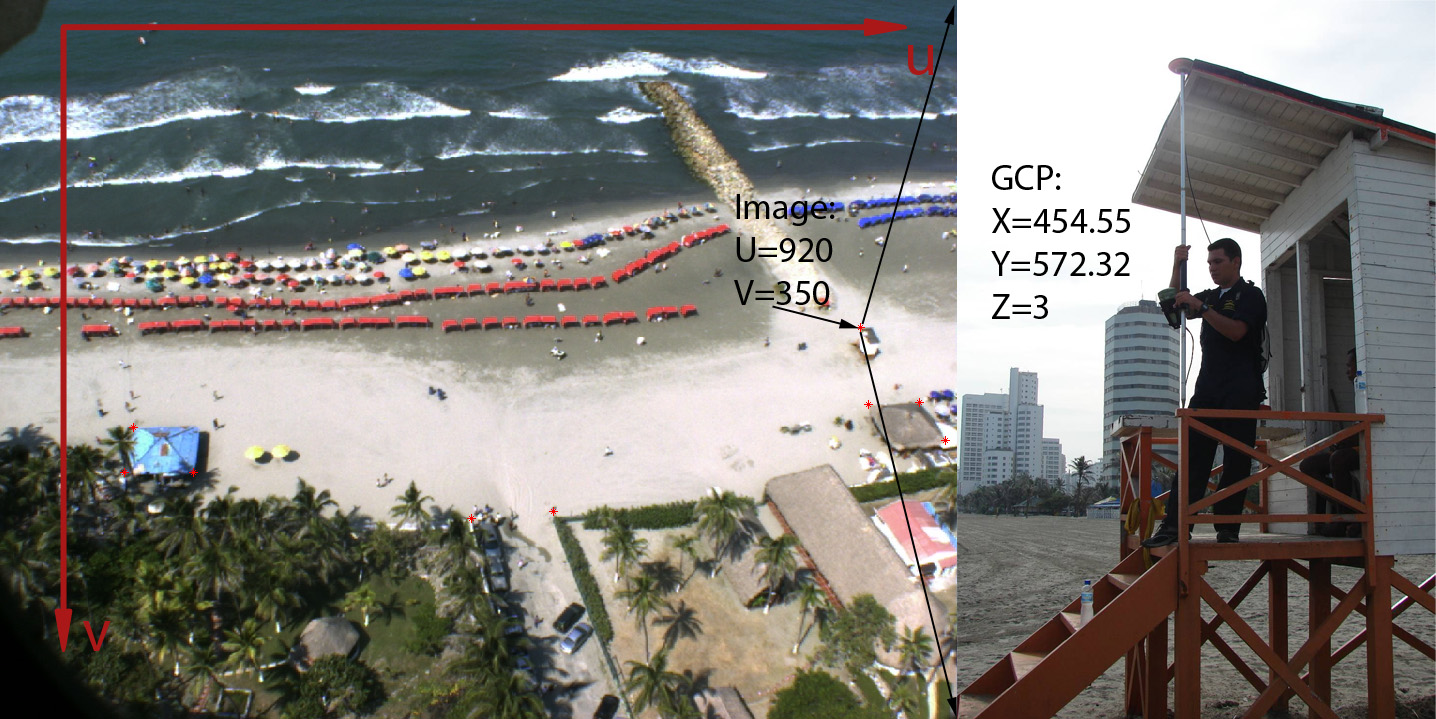
\includegraphics[width=\textwidth]{img/gcp_mark_measure}
  \caption{Relaci�n entre $(u, v)$ y $(x, y, z)$}
  \label{fig:gcp_mark_measure}
\end{figure}

\item[ROI o \textit{Region Of Interest} por su sigla en ingl�s] Un ROI
  es un pol�gono dentro de una imagen que delimita una regi�n de la
  misma. El pol�gono es representado como un conjunto de v�rtices con
  coordenadas $(u, v)$ (medidos en p�xeles) relativos al plano de la
  imagen, tales que cada par de v�rtices consecutivos est�n conectados
  por una l�nea recta. En la figura~\ref{fig:roisample} se muestra un
  ejemplo de ROI en una imagen costera, donde se pueden identificar
  los v�rtices (puntos amarillos) y las l�neas que los unen (l�neas
  rojas) que conforman el pol�gono.

\begin{figure}[htbp!]
  \centering
  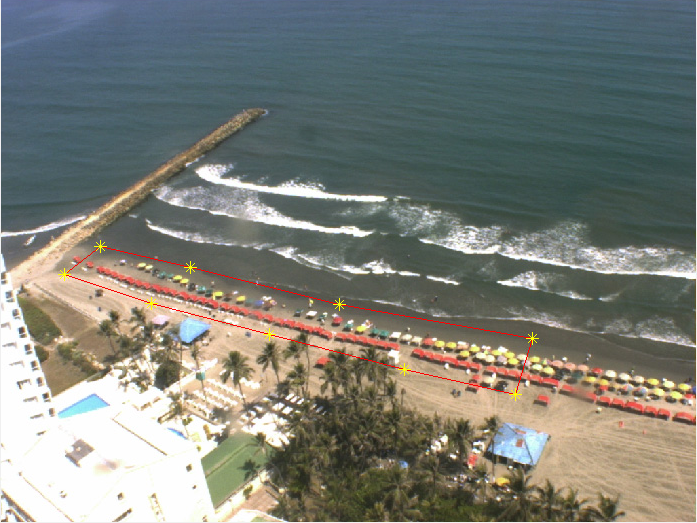
\includegraphics[width=0.6\textwidth]{img/roisample}
  \caption{Ejemplo de un ROI en una imagen}
  \label{fig:roisample}
\end{figure}

\item[Calibraci�n] Es el nombre que se le da al proceso de aplicar un
  m�todo de optimizaci�n para encontrar los par�metros de
  rectificaci�n y fusi�n. La calibraci�n involucra la elecci�n del
  ROI, GCPs, y otros par�metros necesarios para el m�todo.

\item[Imagen Oblicua] Es aquella imagen capturada por una c�mara con
  un �ngulo de inclinaci�n, de tal manera que la imagen tenga una
  perspectiva. En la figura~\ref{fig:oblique} se muestra una imagen
  oblicua.

\begin{figure}[htbp!]
  \centering
  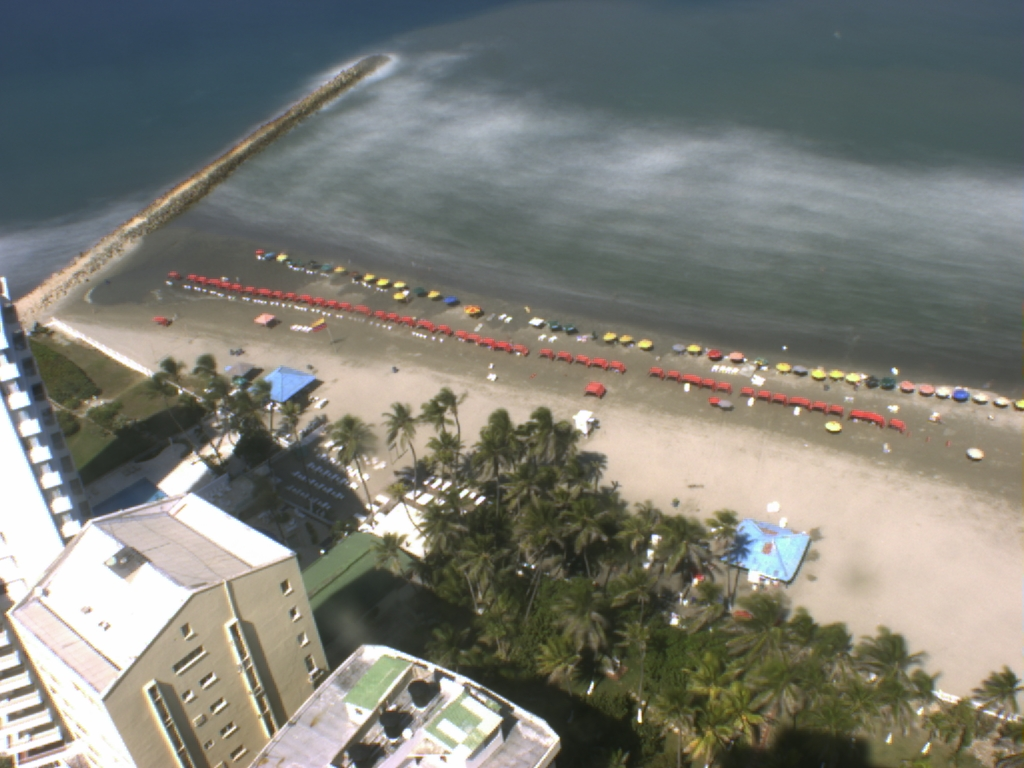
\includegraphics[width=0.6\textwidth]{img/oblique}
  \caption{Ejemplo de imagen oblicua}
  \label{fig:oblique}
\end{figure}

\item[Imagen Rectificada] Es una imagen oblicua que sufre una
  transformaci�n para que parezca como si hubiera sido capturada
  perpendicularmente sobre el plano de la zona de estudio, de tal
  manera que es posible medir distancias y tama�os de objetos dentro
  de la imagen de forma precisa. En la figura~\ref{fig:rectified} se
  muestra un ejemplo de una imagen rectificada.

\begin{figure}[htbp!]
  \centering
  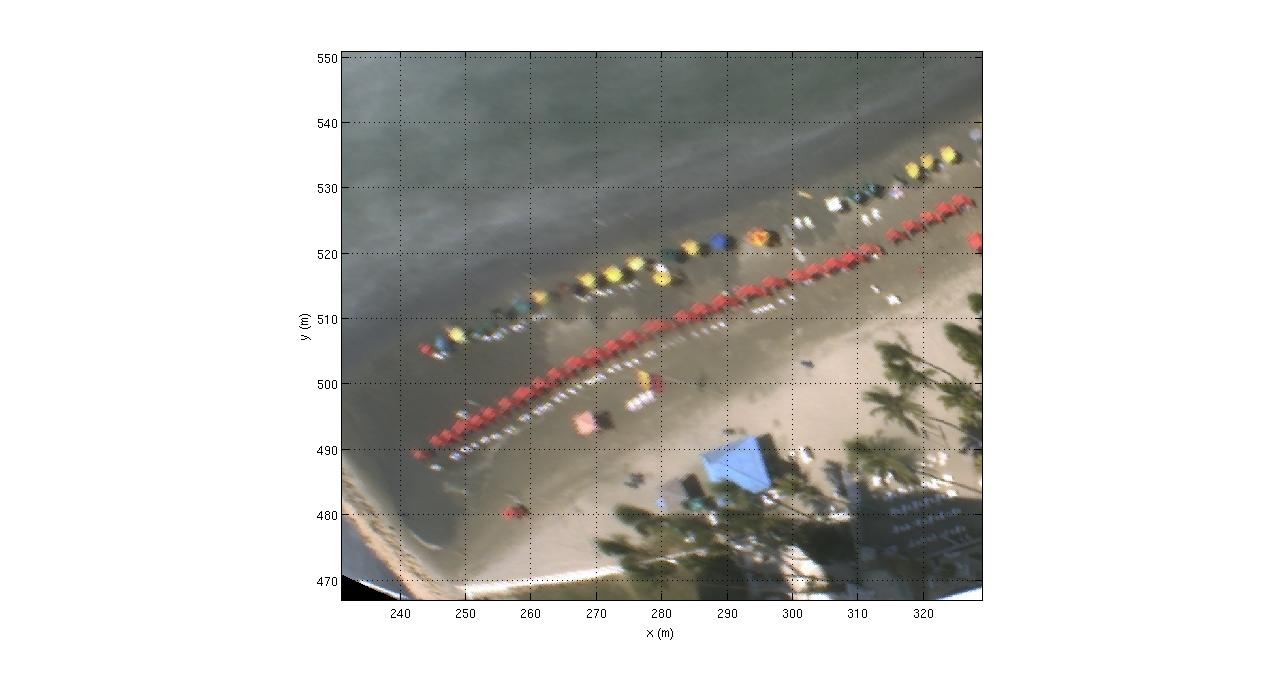
\includegraphics[width=\textwidth]{img/rectified}
  \caption{Ejemplo de imagen rectificada}
  \label{fig:rectified}
\end{figure}

\item[Imagen Fusionada] Es la que resulta de unir dos o m�s im�genes
  (sean oblicuas o rectificadas) por los puntos en com�n entre cada
  par de im�genes consecutivas. Esta fusi�n se realiza rotando y
  distorsionando las im�genes de tal manera que queden acopladas en
  sus puntos comunes, como se muestra en la figura~\ref{fig:merged}.

\begin{figure}[htbp!]
  \centering
  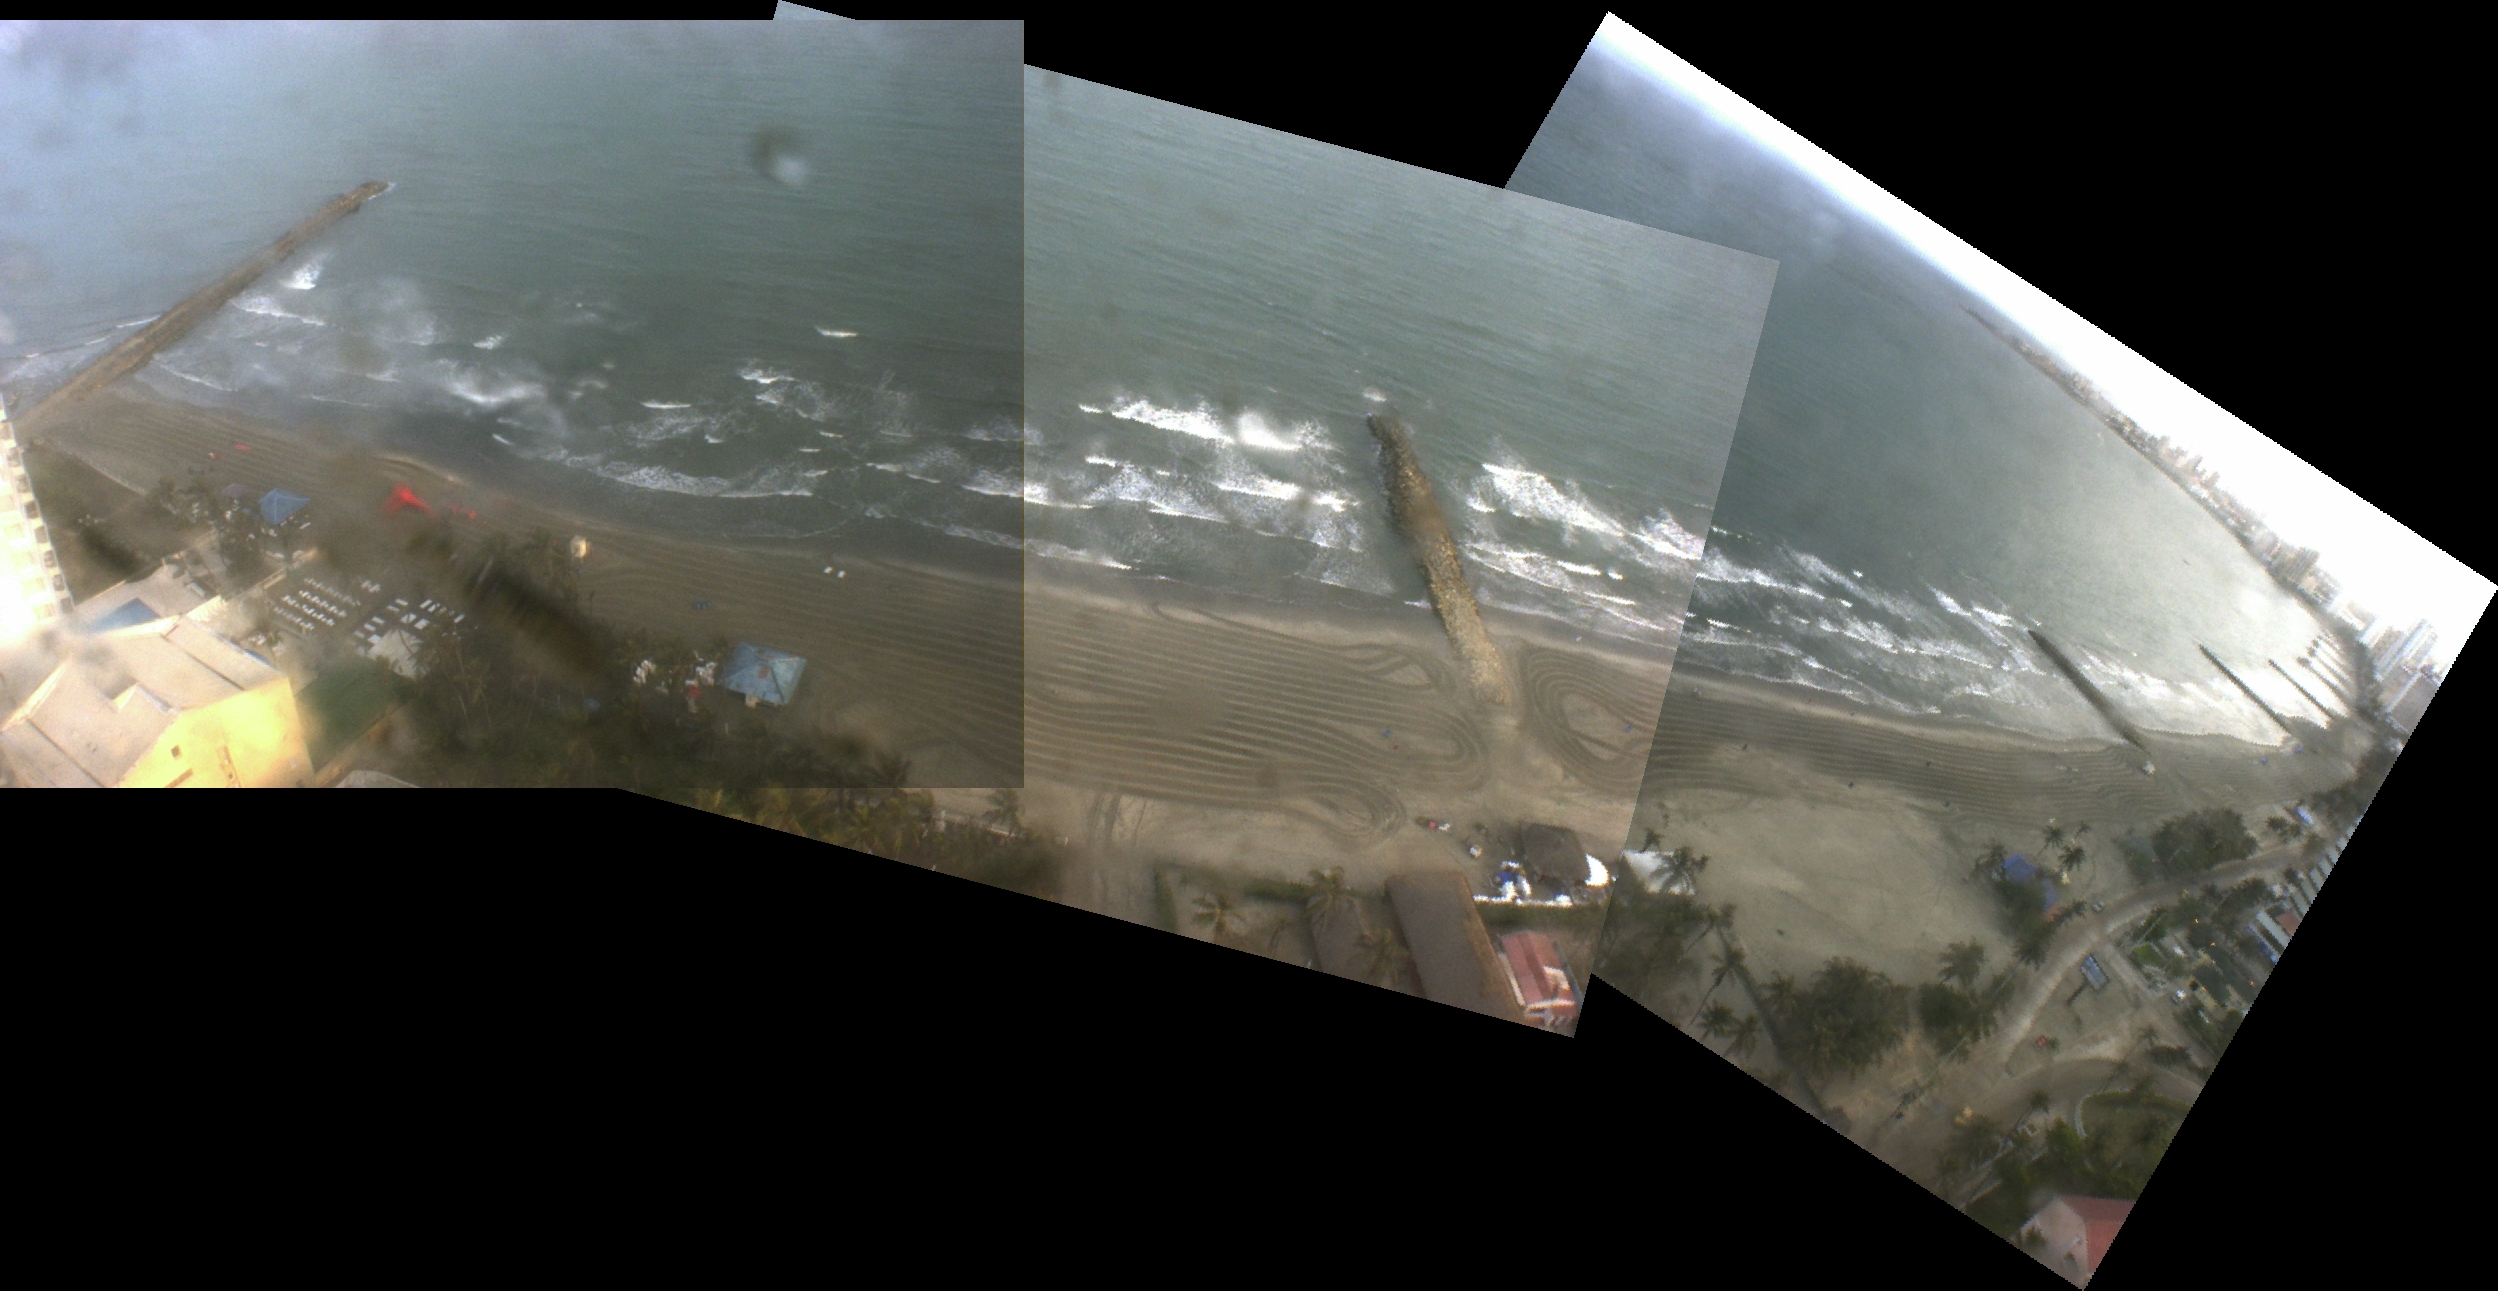
\includegraphics[width=\textwidth]{img/merged}
  \caption{Ejemplo de imagen fusionada}
  \label{fig:merged}
\end{figure}

\item[Imagen \textit{Snap} o \textit{Snapshot}] Una imagen
  \textit{snap} es aquella que es capturada por una c�mara de manera
  instant�nea. Estas im�genes son �tiles para obtener una vista
  est�tica de un evento dado, y mediante una secuencia de estas
  im�genes en el tiempo se puede estudiar la evoluci�n de un
  fen�meno. En la figura~\ref{fig:snapsample} se muestra un ejemplo.

\begin{figure}[htbp!]
  \centering
  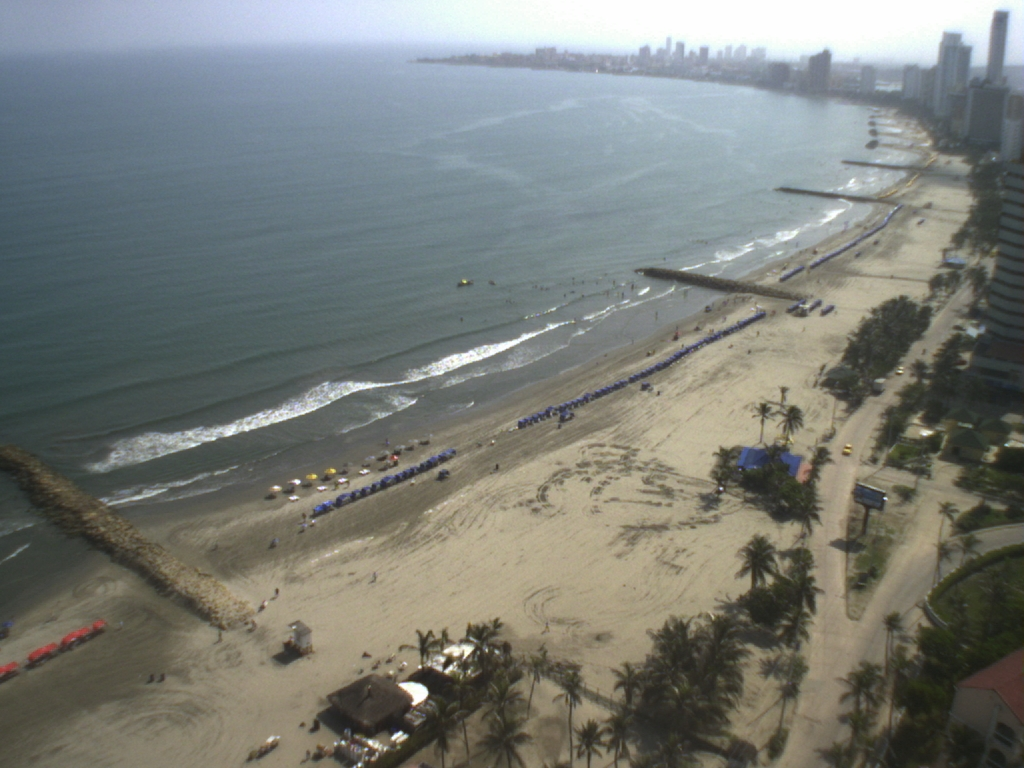
\includegraphics[width=0.6\textwidth]{img/snapsample}
  \caption{Ejemplo de imagen \textit{snap}}
  \label{fig:snapsample}
\end{figure}

\item[Imagen \textit{Timex}] Es el resultado de promediar una
  secuencia de im�genes capturadas a una frecuencia determinada de
  antemano. Estas im�genes son �tiles cuando se quiere generalizar el
  movimiento, es decir, los objetos que tienen mayor variabilidad
  dentro de la imagen se muestran suavizados. Por ejemplo, en la
  figura~\ref{fig:timexsample} se muestra una imagen resultado de
  promediar 120 im�genes a una frecuencia de captura de 2 im�genes por
  segundo, donde el movimiento de las olas, que es el que tiene mayor
  variabilidad es promediado.

\begin{figure}[htbp!]
  \centering
  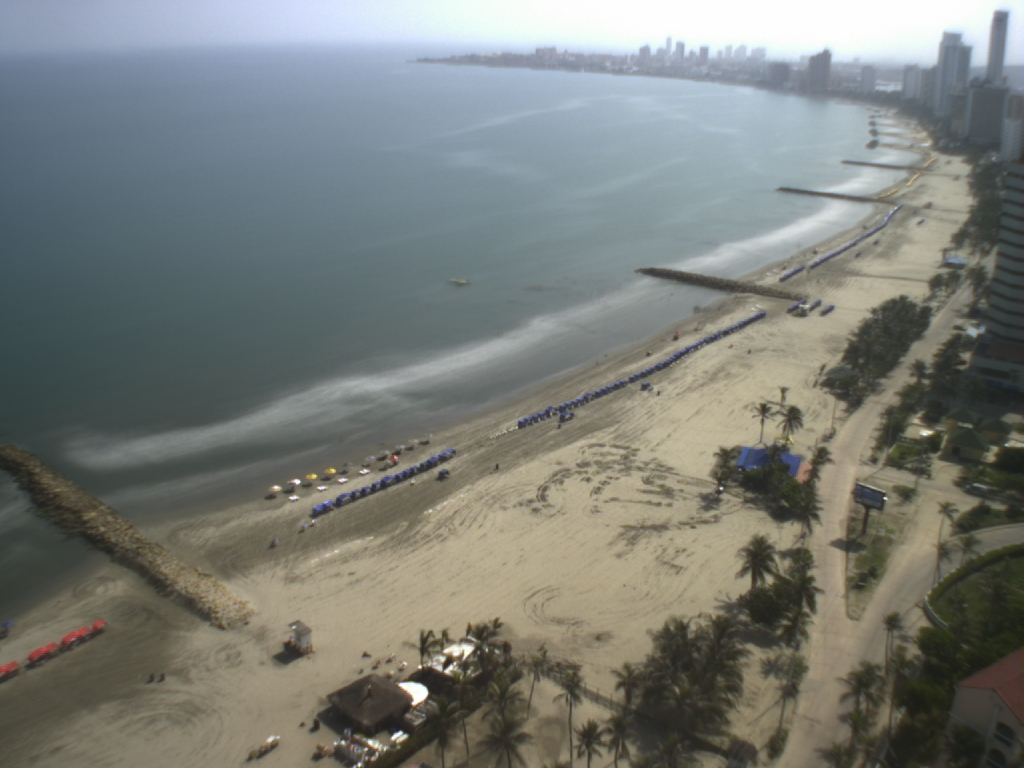
\includegraphics[width=0.6\textwidth]{img/timexsample}
  \caption{Ejemplo de imagen \textit{timex}}
  \label{fig:timexsample}
\end{figure}

\item[Imagen \textit{Variance}] Es el resultado de aplicar la
  desviaci�n est�ndar de una secuencia de im�genes capturadas a una
  frecuencia determinada de antemano. La principal caracter�stica de
  estas im�genes, es que lo que est� en movimiento se muestra en la
  imagen de color claro y lo que est� est�tico se muestra en color
  oscuro. Esto permite resaltar lo que tiene mayor variabilidad en la
  imagen. En la figura~\ref{fig:varsample} se muestra un ejemplo de
  imagen \textit{variance}.

\begin{figure}[htbp!]
  \centering
  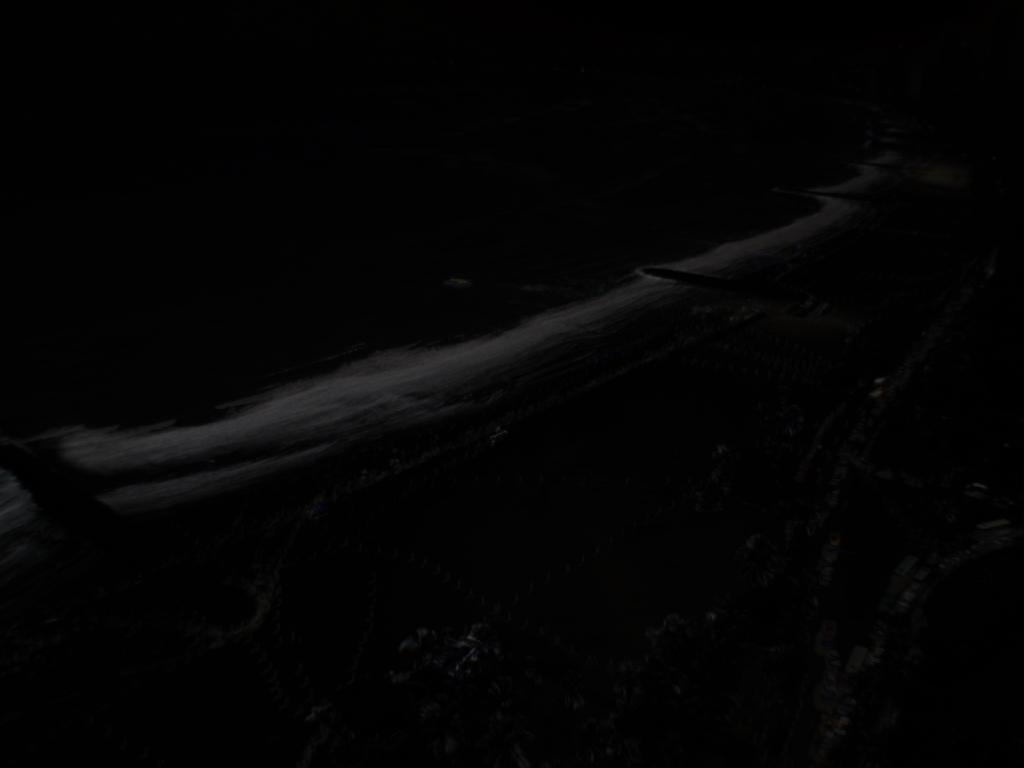
\includegraphics[width=0.6\textwidth]{img/varsample}
  \caption{Ejemplo de imagen \textit{variance}}
  \label{fig:varsample}
\end{figure}

\item[Resoluci�n] Para las im�genes rectificadas, es la resoluci�n
  te�rica deseada de modo que el tama�o de la imagen estar� definido
  por ella y el tama�o del �rea a rectificar en el espacio.  Por
  ejemplo, una regi�n de $10 m \times 10 m$ corresponder� a una imagen
  de $50 pixeles \times 50 pixeles$ si la resoluci�n elegida es $1/5
  (m/pix)$. La resoluci�n de las im�genes oblicuas no es constante
  debido a que el plano de la imagen no es paralelo a la regi�n de
  inter�s o, en otras palabras, la c�mara se encuentra inclinada con
  respecto a dicha regi�n. Como se puede observar en la
  figura~\ref{fig:resolution}, la cual es un mapa de resoluci�n
  obtenido de una imagen oblicua, es posible ver que la resoluci�n de
  la imagen disminuye a medida que el �rea de inter�s est� m�s alejada
  de la c�mara puesto que cada pixel contiene informaci�n de una
  regi�n m�s grande el espacio.

  Es importante notar que no es posible obtener una resoluci�n
  infinitamente alta en la imagen rectificada, porque cuando la
  resoluci�n de la imagen rectificada es menor que la resoluci�n de la
  imagen oblicua en una regi�n determinada el resultado es la p�rdida
  de una porci�n de la informaci�n contenida en la imagen, pero cuando
  la resoluci�n de la imagen rectificada es mayor que la resoluci�n de
  la imagen oblicua, lo que se est� haciendo es forzar que los pixeles
  se estiren, lo que simplemente significa que se usa informaci�n
  redundante para crear la imagen. Por este motivo, la resoluci�n
  usada en la rectificaci�n no deber�a ser mayor que la resoluci�n
  media de la imagen, as� no se pierde demasiada informaci�n pero la
  imagen rectificada tampoco tendr� un gran tama�o, lo cual no es
  pr�ctico.

\begin{figure}[htbp!]
  \centering
  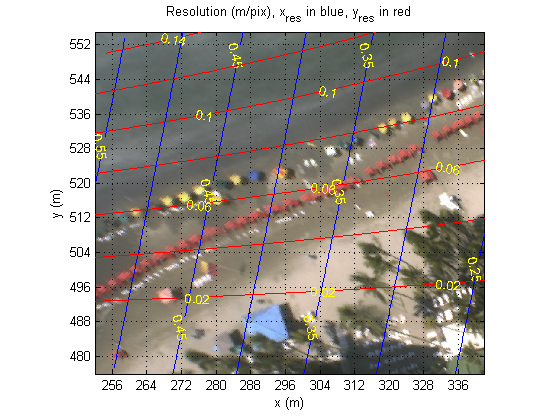
\includegraphics[width=0.6\textwidth]{img/resolution}
  \caption{Mapa de resoluci�n de una imagen oblicua}
  \label{fig:resolution}
\end{figure}

\item[Rectificaci�n] Es el proceso mediante el cual se transforma una
  imagen oblicua como la mostrada en la figura~\ref{fig:oblique} en
  una imagen como la mostrada en la figura~\ref{fig:rectified}. En las
  imagenes oblicuas los objetos en el espacio tienen distinta
  resoluci�n a medida que se alejan o acercan al lente de la
  c�mara. Debido a esto, es imposible hacer mediciones en estas
  im�genes, tales como hallar distancias, o determinar el tama�o de un
  objeto.

  En una estaci�n de monitorizaci�n se tienen varias c�maras que le
  toman fotos a determinadas regiones de la zona de estudio en
  intervalos regulares de tiempo definidos de antemano. En general, es
  necesario convertir las im�genes oblicuas en im�genes rectificadas
  para hacer mediciones de alg�n tipo y extraer informaci�n �til de
  ellas, aplicando m�todos de rectificaci�n basados en un conjunto de
  GCPs. Los m�todos con los que se cuenta son \textit{DLT}
  \cite{faugueras93,hartley03,salvi02,wolf00} (Transformada Lineal
  Directa), \textit{RANSAC--DLT} \cite{perez09} y \textit{Pinhole}
  \cite{hartley03,holland97,osorio07,salvi02}.

  El proceso de rectificaci�n de im�genes se esquematiza en la
  figura~\ref{fig:geom_rectification}.

  \begin{landscape}
    \begin{figure}[htbp]
      \centering
      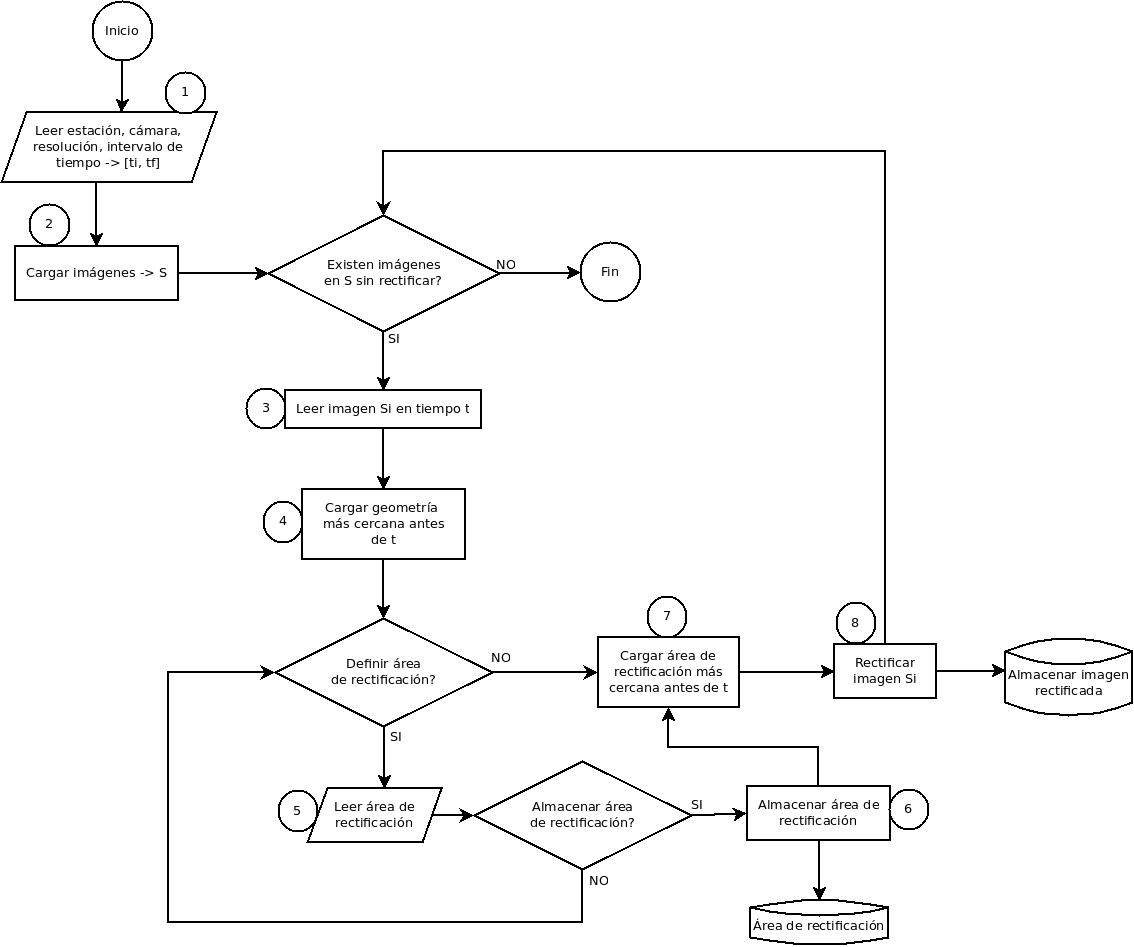
\includegraphics[width=0.8\linewidth]{img/geom_rectificacion}
      \caption{Diagrama de flujo de la rectificaci�n en HORUS}
      \label{fig:geom_rectification}
    \end{figure}
  \end{landscape}

  Los pasos en el proceso de rectificaci�n son los siguientes:
  \begin{enumerate}
  \item El usuario ingresa la estaci�n, c�mara, resoluci�n e intervalo
    de tiempo en el cual se van a rectificar im�genes.
  \item Se cargan todas las im�genes que correspondan a este intervalo
    de tiempo en el conjunto S y que correspondan a la estaci�n y
    c�mara que se ingresaron.
  \item Mientras hayan im�genes sin rectificar en el conjunto de
    im�genes S, se lee cada imagen.
  \item Se carga la calibraci�n de rectificaci�n m�s cercana antes del
    tiempo de la imagen actual.
  \item Si el usuario decide definir el ROI de rectificaci�n en la
    imagen, se lee el ROI de rectificaci�n manualmente. Este proceso
    se repite tantas veces como se requiera.
  \item Cuando el usuario est� conforme con el ROI de rectificaci�n,
    se almacena.
  \item Se carga el ROI de rectificaci�n m�s cercano antes del tiempo
    de la imagen.
  \item Se rectifica la imagen teniendo en cuenta los par�metros de
    rectificaci�n y el ROI de rectificaci�n y se almacena la imagen
    rectificada.
  \end{enumerate}

\item[Fusi�n] En el proceso de fusi�n se generan los par�metros que
  sirven para unir dos im�genes a trav�s de unos puntos conocidos en
  com�n. En la figura~\ref{fig:fusionprocess} se esquematiza el
  proceso para generar una fusi�n entre dos im�genes. Cuando se
  calibra la fusi�n se llevan a cabo los siguientes pasos: Primero, se
  elige un conjunto de puntos comunes entre las dos im�genes (en la
  figura~\ref{fig:fusionprocess} estos puntos corresponden al
  tri�ngulo tanto dentro de la imagen de la izquierda como en la
  imagen de la derecha); se genera una matriz de transformaci�n que es
  la que permite unir estos puntos en com�n rotando y/o distorsionando
  una de las im�genes para que coincida con la otra imagen en sus
  puntos comunes. Finalmente, las dos im�genes se unen en una sola.

  En HORUS se cuenta con dos m�todos para estimar las matrices de
  transformaci�n, cuando la fusi�n es para im�genes oblicuas:
  transformaci�n af�n y transformaci�n proyectiva. La primera se
  emplea cuando la diferencia entre las im�genes es una traslaci�n o
  peque�a rotaci�n de la c�mara. La transformaci�n proyectiva es buena
  tanto para estos movimientos como para diferencias m�s grandes en la
  orientaci�n de las c�maras. Para la fusi�n de im�genes rectificadas
  se debe utilizar la transformaci�n af�n, ya que las diferencias en
  la orientaci�n han sido corregidas.

  Para la transformaci�n af�n se requieren m�nimo tres puntos comunes,
  mientras que para la transformaci�n proyectiva se requieren m�nimo
  cuatro puntos en com�n. Cuando el n�mero de puntos en com�n es alto,
  se puede optimizar el c�lculo de la matriz de transformaci�n
  mediante el m�todo de optimizaci�n \emph{Levenberg--Marquardt}.

\begin{figure}[htbp!]
  \centering
  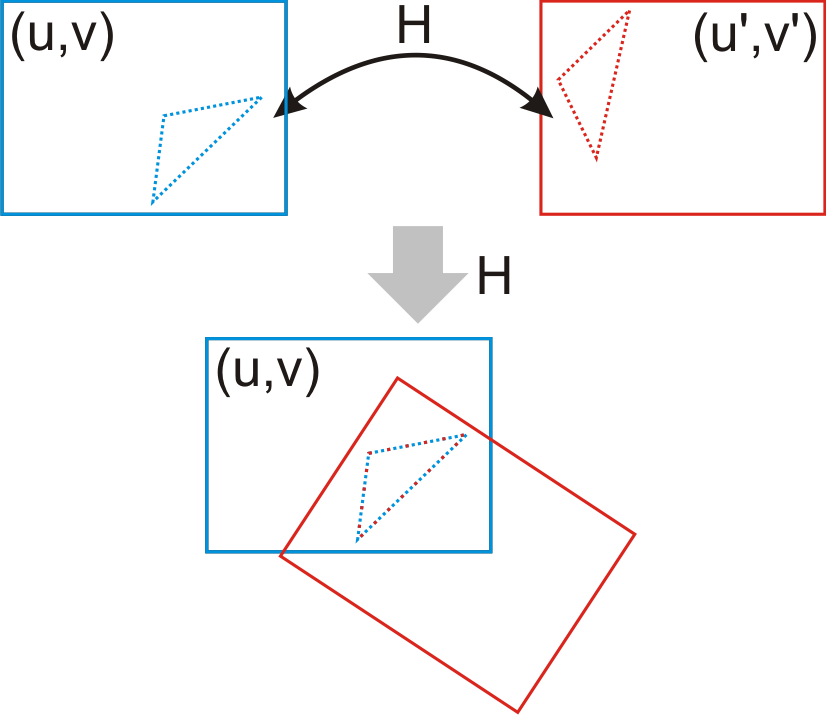
\includegraphics[width=0.6\textwidth]{img/fusionprocess}
  \caption{Esquema de la fusi�n entre dos im�genes}
  \label{fig:fusionprocess}
\end{figure}

En el sistema HORUS se capturan im�genes de la zona de estudio que
adem�s de ser rectificadas tambi�n pueden ser fusionadas, dado que
cada par de im�genes de c�maras consecutivas tengan puntos en
com�n. El usuario puede marcar puntos en un par de im�genes que
corresponden a las mismas coordenadas geogr�ficas. Estas marcaciones
sirven como insumo para generar los par�metros del modelo que fusiona
las im�genes.

El proceso de fusionar im�genes en HORUS se esquematiza en la
figura~\ref{fig:fusiondesign}.

\begin{figure}[htbp] \centering
  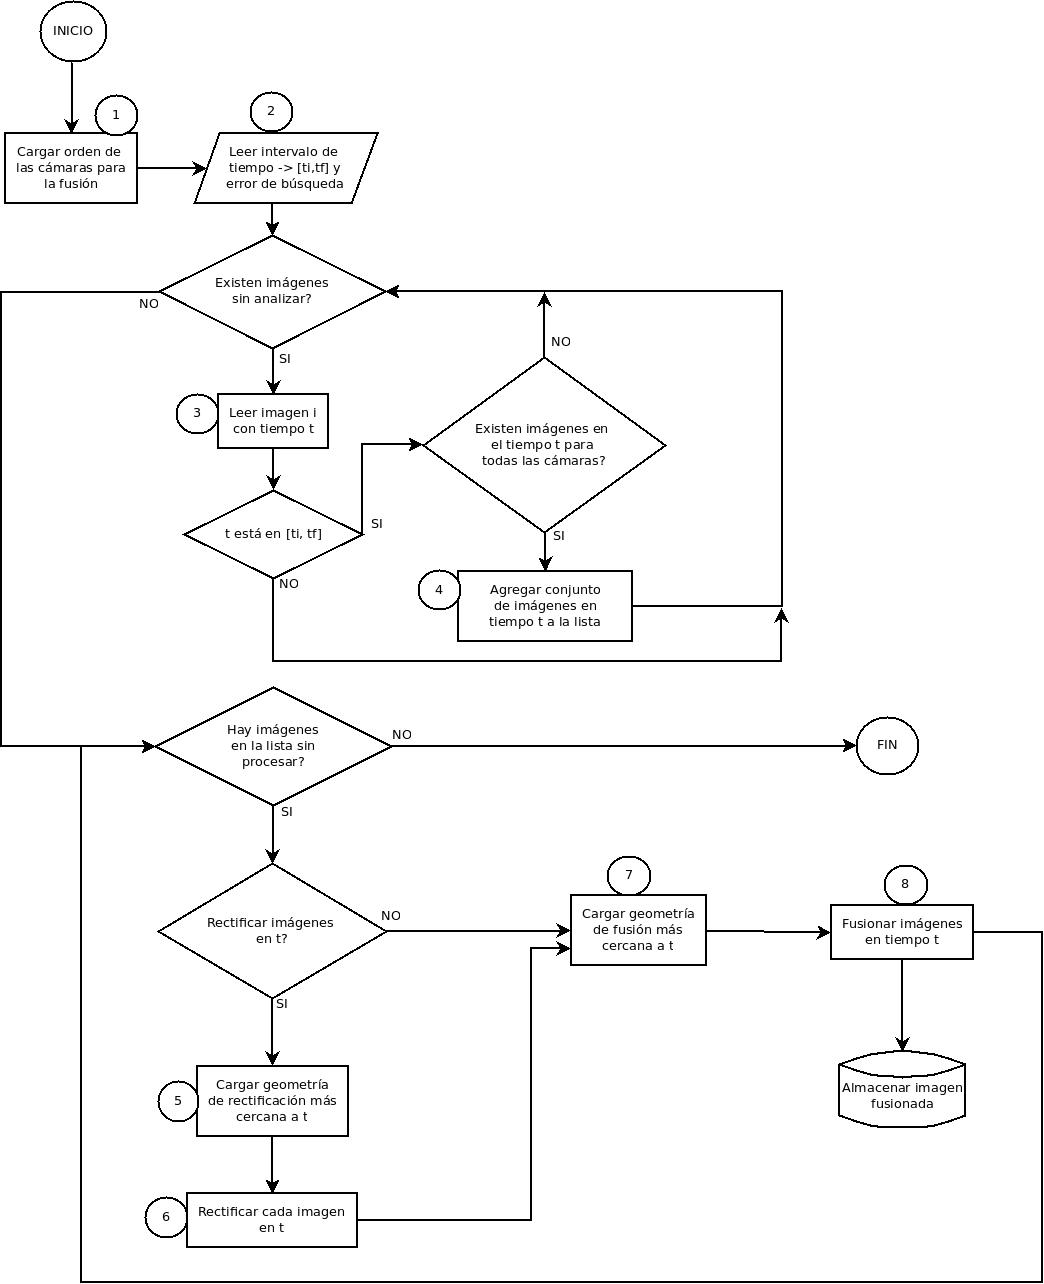
\includegraphics[width=1.0\linewidth]{img/fusiondesign}
  \caption{Diagrama de flujo de la fusi�n en HORUS}
  \label{fig:fusiondesign}
\end{figure}

Los pasos que se llevan a cabo en el proceso de fusi�n son los
siguientes:
\begin{enumerate}
\item El primer paso es cargar el orden de las c�maras para la
  fusi�n. Cuando se definen los par�metros de una fusi�n, se debe
  definir cu�les son las c�maras que participan en la fusi�n y en qu�
  orden, esto es porque el m�todo utiliza este orden para
  fusionar las im�genes de cada c�mara.
\item La fusi�n se realiza en un intervalo de tiempo especificado por
  el usuario. Se buscan todas las im�genes en este intervalo. El error
  corresponde al margen para buscar im�genes coincidentes para todas
  las c�maras en un tiempo espec�fico, ya que es posible que las
  im�genes difieran por unos pocos segundos.
\item Para todas las im�genes que est�n en el intervalo de tiempo, se
  lee cada una para ser procesada secuencialmente.
\item Se verifica que para el instante de tiempo (+/- error) de cada
  imagen existan im�genes para todas las c�maras presentes en el
  orden. Si hay im�genes para todas las c�maras, se agregan a la
  lista.
\item Si se especific� que las im�genes se rectifican antes de
  fusionar, para cada imagen en la lista de conjuntos de im�genes se
  carga la calibraci�n m�s cercana antes del tiempo de las im�genes,
  para rectificarlas.
\item Se rectifican la im�genes con los par�metros cargados, y se
  reemplazan las im�genes originales con la rectificadas.
\item Despu�s de que se rectifican las im�genes para el tiempo actual,
  si se especific� que se rectificaran, o no, se procede a fusionar
  las im�genes. Se cargan los par�metros de la fusi�n m�s cercanos
  antes del tiempo de las im�genes.
\item Se fusionan todas las im�genes en el conjunto de im�genes y se
  almacenan. Mientras hayan m�s im�genes por procesar, se repite el
  proceso.
\end{enumerate}

\item[\textit{Timestamp}] Representa el tiempo de un objeto o evento
  que contiene la fecha y hora en un formato espec�fico. Para el resto
  de este manual, este tiempo es representado por un valor num�rico,
  el n�mero de d�as desde enero $1$ del a�o $0$ m�s $1$. �ste es el
  mismo formato que utiliza la funci�n \texttt{datenum} de MATLAB\@.

\item[Hosting o almacenamiento web] Es un servicio que ofrecen algunas
  compa��as en Internet donde ceden un espacio en sus servidores para
  subir (alojar) un sitio web para que pueda ser accedido de forma
  online.
  
\item[Servidor de archivos] Es un computado que almacena varios
  tipos de archivos, en este caso im�genes, y puede ser accedido desde
  otros computadores de forma online que reciben el nombre de
  clientes.

\item[Base de datos sat�lite] Una base de datos es una colecci�n de
  informaci�n organizada de forma que un software pueda seleccionar
  r�pidamente los fragmentos de datos que necesite. Se le asigna el
  nombre de base de datos sat�lite a aquella que s�lo posee
  informaci�n de una o m�s estaciones pero no de todas.

\item[Base de datos central] Se le asigna el nombre de base de datos
  central a aquella que posee la informaci�n de todas las base de
  datos sat�lites.
 
\item[Base de datos hosting] Se le asigna el nombre de base de datos
  \textit{hosting} a aquella que se encuentra en el \textit{hosting} y
  posee la informaci�n de la base de datos central, y hace las veces
  de respaldo en un servidor externo.
  
\item[Timestack] Es una matriz de series temporales de intensidad de
  pixel de una regi�n de inter�s, en palabras coloquiales se puede
  definir como una secuencia de im�genes de una regi�n de inter�s en
  el tiempo a cierta frecuencia de muestreo. En la
  figura~\ref{fig:timestack} se ve como se selecciona una regi�n de
  inter�s de un timestack en \textit{cross-shore} o
  \textit{alongshore} (l�nea roja y l�nea amarilla
  respectivamente). En HORUS los \textit{timestacks} se capturan y
  almacenan como videos que contienen la secuencia de im�genes.
  
\begin{figure}[htbp!]
  \centering
  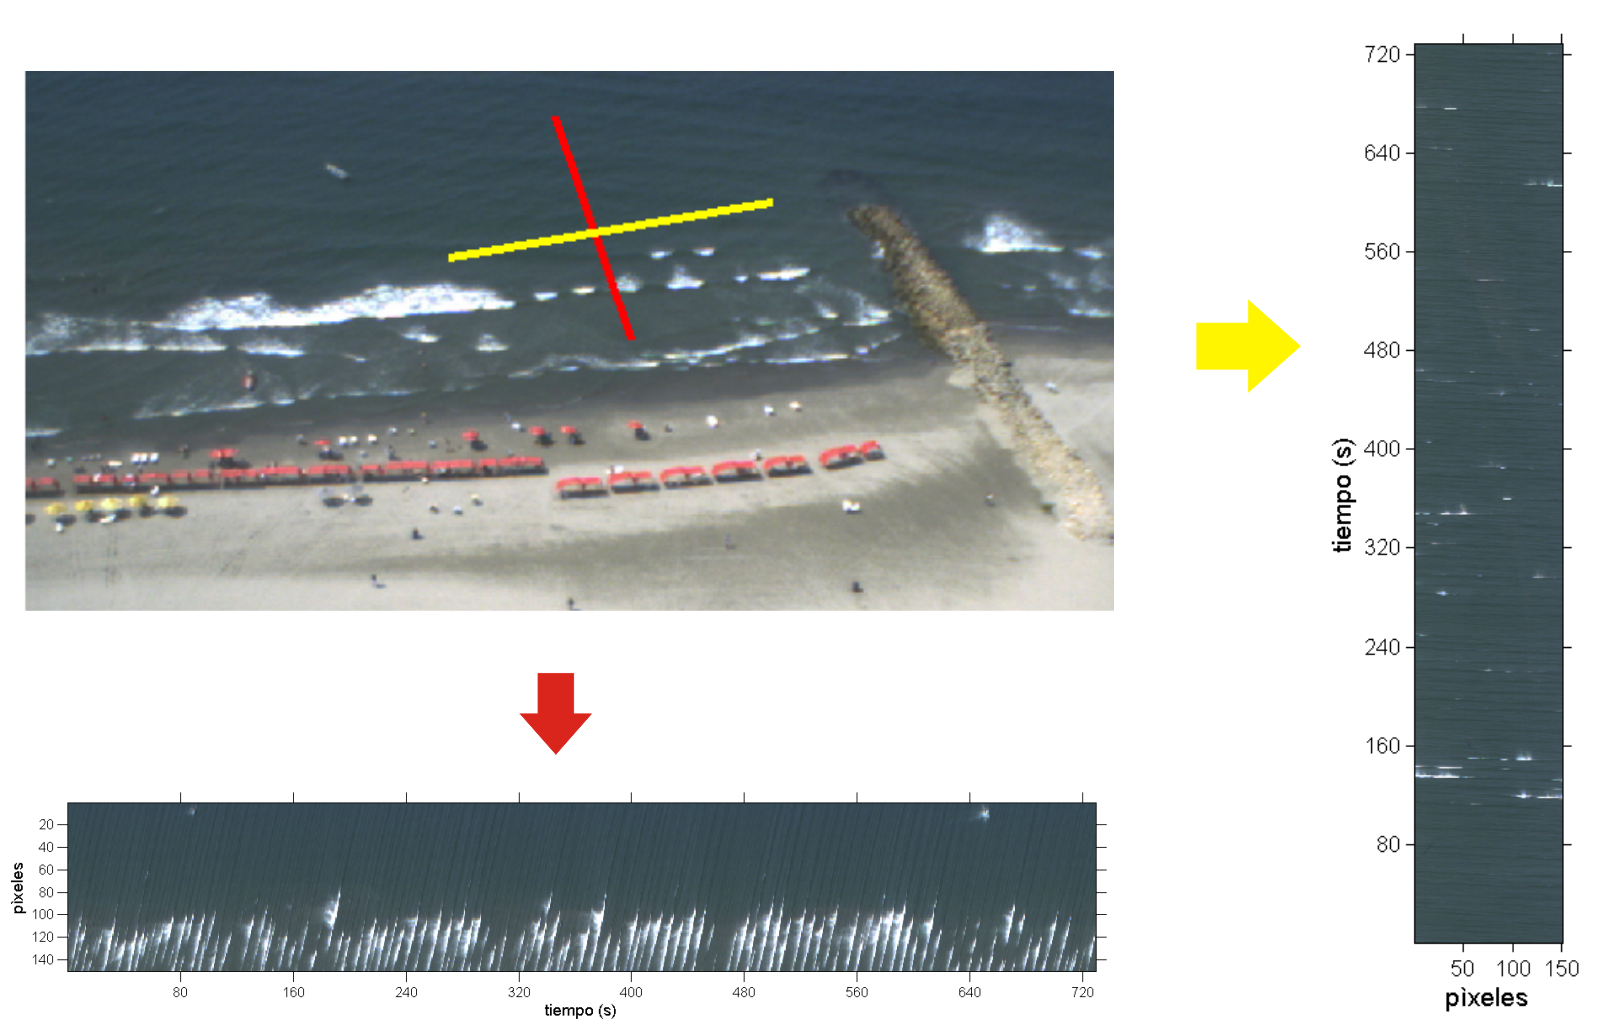
\includegraphics[width=\textwidth]{img/timestack}
  \caption{Selecci�n de una regi�n para un timestack}
  \label{fig:timestack}
\end{figure}
  
\item[Frame o fotograma] Es una imagen particular dentro de una
  sucesi�n de im�genes que conforman un video, al hablar de n�mero de
  frames se hace referencia a cuantas im�genes va a tener el video.
  
\end{description}


\chapter{Introducci�n}
\label{chap:intro}

HORUS es un sistema de monitorizaci�n ambiental que consiste en varias 
estaciones ubicadas en lugares espec�ficos, donde hay c�maras
que toman fotos peri�dicamente desde distintos �ngulos a una regi�n de
la zona de estudio. Las im�genes tomadas por las c�maras son
procesadas mediante algoritmos avanzados con el fin de extraer
informaci�n �til de ellas.
\\


El sistema HORUS est� compuesto por los m�dulos de captura,
procesamiento y visualizaci�n en la web, como se muestra en la
figura~\ref{fig:scheme}. Cada una de estas componentes tiene asociado
un conjunto de funciones escritas en el lenguaje de MATLAB para las
tareas de procesamiento, almacenamiento y extracci�n de
informaci�n. Estas funciones est�n ligadas con una base de datos
sat�lite que almacena toda la informaci�n necesaria para procesar las
im�genes y proveer informaci�n �til tanto para gestores, y cient�ficos
como para investigadores. En la figura ~\ref{fig:scheme_db} se explica
el funcionamiento de HORUS con las bases de datos, en esta figura cada
servidor de captura ser� configurado con un $\Delta$t que indica cada
cu�nto tiempo se har� la captura y la transferencia de la informaci�n,
�ste ser� escogido por los administradores de la estaci�n dependiendo
de sus necesidades. El $\Delta$t puede ser diferente o no para todos
los procesos de captura, transferencia de informaci�n y procesamiento 
de las im�genes, estos procesos son independientes entre s�. 
\\

\begin{figure}[htbp!]
  \centering
  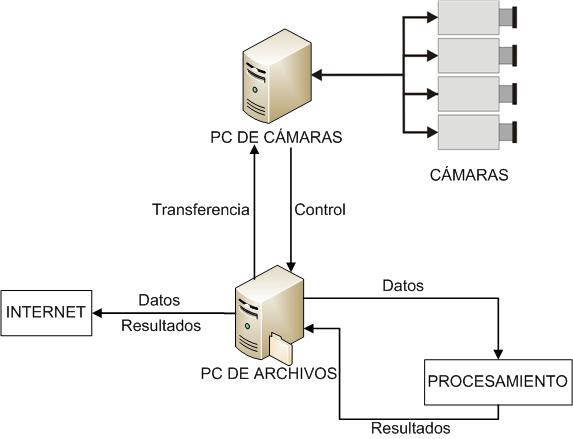
\includegraphics[width=0.8\textwidth]{img/scheme}
  \caption{Esquema general de HORUS}
  \label{fig:scheme}
\end{figure}

\begin{figure}[htbp!]
  \centering
  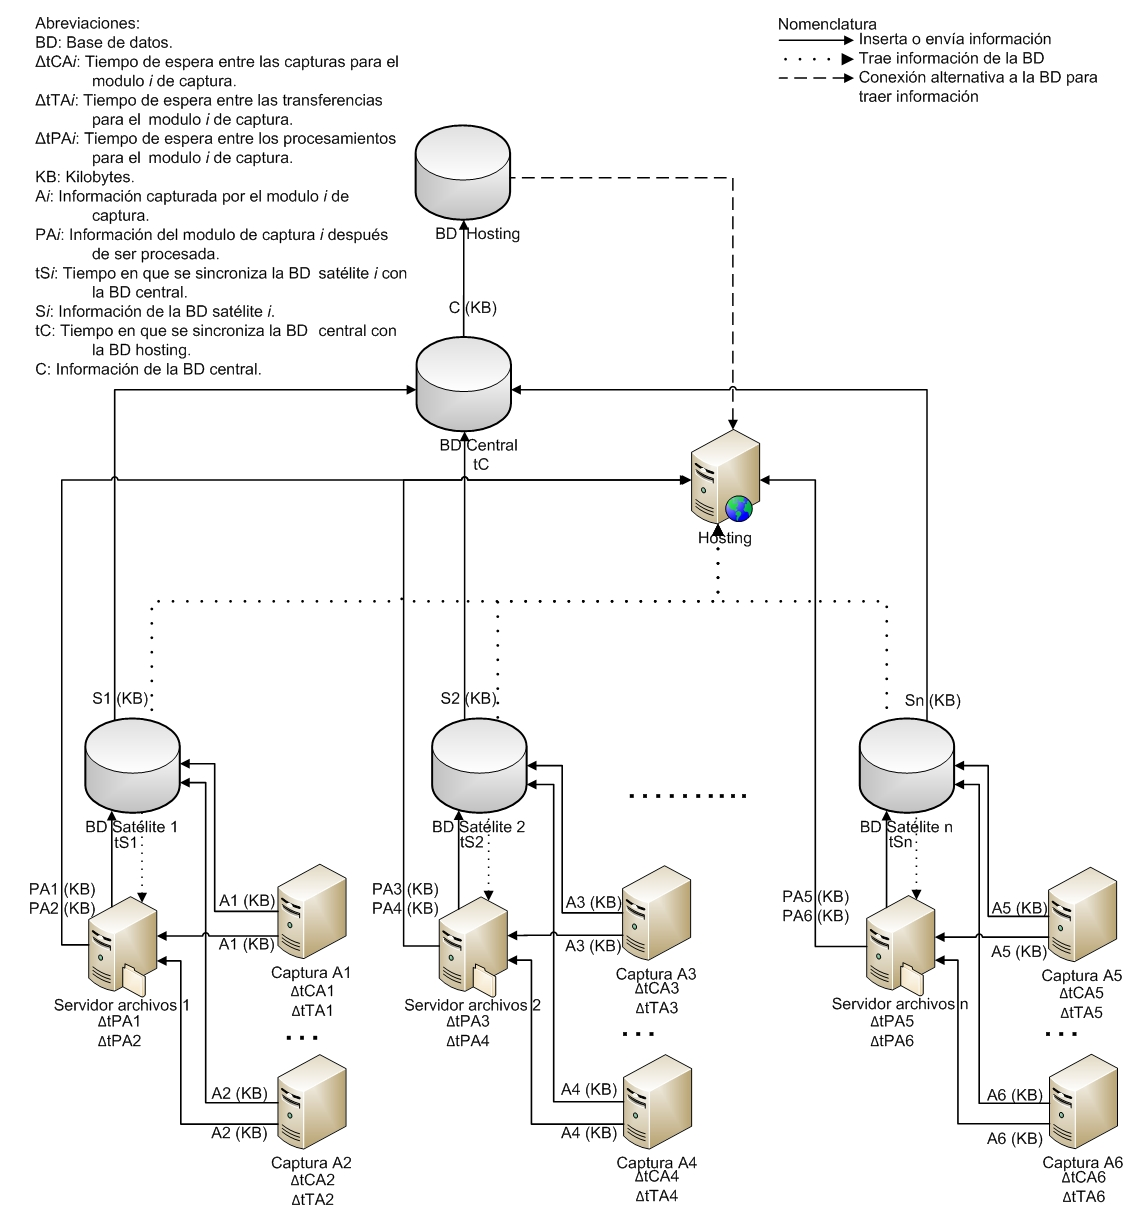
\includegraphics[width=\textwidth]{img/scheme_db}
  \caption{Esquema de funcionamiento completo de HORUS}
  \label{fig:scheme_db}
\end{figure}

En el proceso de transferencia de informaci�n se env�an las im�genes a
un servidor de archivos, y se env�a la informaci�n de la imagen tal 
como su nombre, la ruta relativa donde ser� guardada, la fecha de captura, 
entre otra informaci�n a una base de datos sat�lite. El servidor de archivos 
y la base de datos sat�lite pueden o no estar en el mismo equipo.  Para 
calcular los KB (Kilobytes) que se env�an al servidor de archivos se debe 
sumar el peso de todas las im�genes tomadas en una captura, y para 
calcular los KB enviados a la base de datos se debe multiplicar la cantidad 
de im�genes tomadas en una captura por 0.5 KB (de acuerdo a los tama�os de los campos
definidos en la base de datos). En la etapa de procesamiento lo que se haga 
va a depender de las opciones que haya seleccionado el administrador de la 
estaci�n pero en forma general se fusionan las im�genes oblicuas y se fusionan 
las im�genes rectificadas de tipo snap y timex y se generan miniaturas de estas 
fusiones y de las im�genes oblicuas de tipo snap y timex, a medida que se van 
generando las nuevas im�genes estas son insertadas en la base de datos sat�lite, 
por �ltimo en este proceso se env�an las im�genes miniaturas al \textit{hosting}. 
\\

Las bases de datos sat�lites env�an informaci�n cada $t$ (puede ser
una vez al d�a en horas de la noche) a la base de datos central en donde se 
concentrar� toda la informaci�n de las bases de datos sat�lites. La base de 
datos central enviar� su informaci�n tambi�n cada $t$ a la base de datos 
del \textit{hosting} que har� las veces de respaldo de los datos.
 Entre el \textit{hosting} y las bases de datos sat�lites habr� una comunicaci�n 
 permanente ya que el \textit{hosting} consulta estas bases de datos para poder
mostrar las im�genes en la p�gina web. En caso de que haya problemas
de conexi�n entre �stos, el \textit{hosting} utilizar�a la base de datos que
est� almacenando para mostrar la informaci�n aunque no sea la �ltima
generada, por esta raz�n en la figura la conexi�n entre estos es
punteada. 
\\

A continuaci�n se plantea un ejemplo de un caso hipot�tico para que se entienda 
mejor el funcionamiento del sistema HORUS. Para empezar se supone que se tiene un 
sistemas de captura que llamaremos CARTAGENA que cuenta con tres c�maras, 
este se comunica con el sistema de archivos A1 y con la base de datos sat�lite S1. 
Se debe comenzar definiendo la hora de inicio y fin de la captura de im�genes para 
este caso ser�n 6:30 y 18:30 respectivamente. Ahora se definir� el $\Delta$t para 
saber cada cuanto se ejecutar� la captura el cual va a ser de 30 minutos. Luego se 
definen los tipos de im�genes a capturar en este caso ser�n snap, timex y var. Ahora 
se debe definir de cuanto es el tiempo de captura de las im�genes timex y var el 
cual ser� de 120 segundos. 
\\

Ahora se configurar� la captura de timestack, se empieza escogiendo la hora de inicio 
y fin que ser� 10:10 y 16:10 respectivamente, el $\Delta$t es de 120 minutos y 
el n�mero de frames es de 1200.
\\

Despu�s de esto se configura la transferencia de las im�genes capturadas, se comienza 
escogiendo la hora de inicio y fin que ser� 6:40 y 18:40 respectivamente y el $\Delta$t 
que ser� de 30 minutos. Al ejecutarse enviara las im�genes capturadas a A1 e insertara 
la informaci�n de las im�genes en S1.
\\

Por �ltimo se debe configurar el proceso de procesamiento en el sistema de archivos A1, 
en el cual se pondr� la hora de inicio y fin con 6:50 y 18:50 respectivamente y el 
$\Delta$t que ser� de 30 minutos, en este tambi�n se configuran las opciones que se 
quieren procesar que ser�n fusionar im�genes oblicuas y fusionar im�genes rectificadas 
de tipo snap y timex, generar miniaturas de estas fusiones y de im�genes oblicuas de tipo 
snap y timex, y se configuran los datos para transferir las miniaturas al \textit{hosting}. 
Este cada que se ejecuta genera las im�genes que se configuraron e inserta la informaci�n de 
estas en S1, por ultimo sube las im�genes miniaturas al \textit{hosting}.

Para mayor informaci�n de c�mo hacer estas configuraciones vaya al apartado de autom�ticos ~\ref{sect:processconf}.

En la tabla~\ref{table:intro_conf} se puede ver el resumen de la informaci�n suministrada para configurar la captura.

\begin{table}[!hbt]
  \label{table:intro_conf}
  \begin{center}
    \begin{tabular}{|l|c|c|c|c|}
      \hline
      \multicolumn{5}{|c|}{CARTAGENA}\\
      \hline
      \multirow{2}{*}{\emph{Informaci�n}} & \emph{Captura} &  \emph{Captura} &   \emph{Transferencia} & \multirow{2}{*}{\emph{Procesamiento}} \\
      & \emph{im�genes} & \emph{timestack} & \emph{im�genes} & \\
      \hline
      \emph{Hora de inicio} & 6:30 & 10:10 & 6:40 & 6:50 \\
      \hline
      \emph{Hora de fin} & 18:30 & 16:10 & 18:40 & 18:50 \\
      \hline
      \emph{$\Delta$t (min)} & 30 & 120 & 30 & 30 \\
      \hline
      \emph{Tipos de im�genes} & snap, timex y var & \- & \- & snap y timex\\
      \hline
      \emph{Tiempo captura} & \multirow{2}{*}{120} & \multirow{2}{*}{\-} & \multirow{2}{*}{\-} & \multirow{2}{*}{\-} \\
      \emph{(timex y/o var)} & & & & \\
      \hline
      \emph{N�mero de frames} & \- & 1200 & \- & \- \\
      \hline
    \end{tabular}
    \caption[Resumen configuraci�n]{Resumen configuraci�n}
  \end{center}
\end{table}

En la figura~\ref{fig:time_line} se muestra una l�nea de tiempo de los procesos antes configurados, 
para poder evaluar si los tiempos si son los adecuados y que no se est�n solapando 
cuando no lo deben hacer. Estos tiempos se calculan con las siguientes formulas:

\begin{itemize}
\item \emph{Captura}: \\
3*duracion [seg]
\\
Para hacer este c�lculo se est� poniendo una holgura de dos veces la duraci�n de la 
captura para que el sistema procese las im�genes capturadas y obtener las im�genes de tipo timex y var.
\item \emph{Timestack}: \\
1.4*duracion2 [seg]
\\
Para este c�lculo se est� poniendo una holgura del 40\% del tiempo de captura de los timestack 
para que se procesen las im�genes  y se guarde el video.
\item \emph{Transferencia}: \\
25*imagenes [seg]
\\
Para el c�lculo de este se asume una velocidad de 20 KB/s y un peso por imagen de 500 KB  
ya que la velocidad se asume baja en esta se tiene en cuenta la holgura.
\item \emph{Procesamiento}: \\
1.4*((29*imagenes)+210) [seg]
\\
Para el c�lculo de este se hicieron pruebas y se llego a que se demora 29 
segundos procesando cada imagen y se demora en total 210 segundos en pasar entre 
los diferentes procesos y por �ltimo se est� asumiendo una holgura del 40\% para 
hacer el procesamiento de todas las im�genes.
\end{itemize}
Donde:
\\
duracion: Tiempo de captura para im�genes tipo timex o var.
\\
duracion2: (numero de frames)/(frame rate), es decir el tiempo de duraci�n del timestack.
\\
imagenes: Cantidad de im�genes capturadas.


\begin{figure}[htbp!]
  \centering
  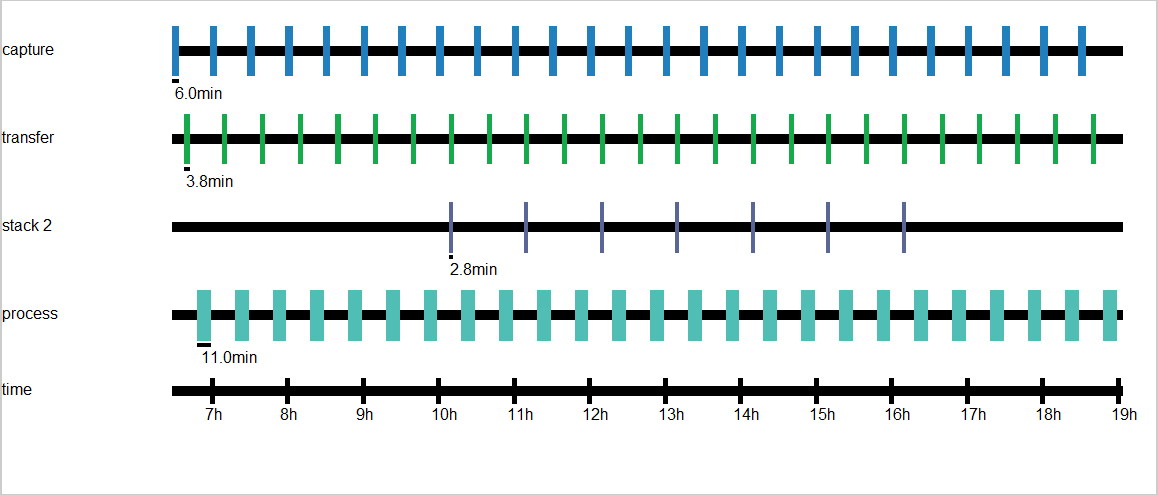
\includegraphics[width=\textwidth]{img/time_line}
  \caption{L�nea de tiempo de los procesos}
  \label{fig:time_line}
\end{figure}

En este manual se describen las interfaces gr�ficas que acompa�an a
las funciones que componen el Toolbox, las cuales son una ayuda para
el usuario que desea realizar tareas de administraci�n, manipulaci�n y
procesamiento de la informaci�n de manera asistida, aunque tambi�n es
posible utilizar las rutinas independientemente.



\chapter{Dise�o de HORUS}
\section{Estructura del Toolbox}
\label{sec:horusdesign}

El sistema HORUS es un paquete con la estructura que se muestra en
la figura~\ref{fig:dir}.

\begin{figure}[htbp] \centering
  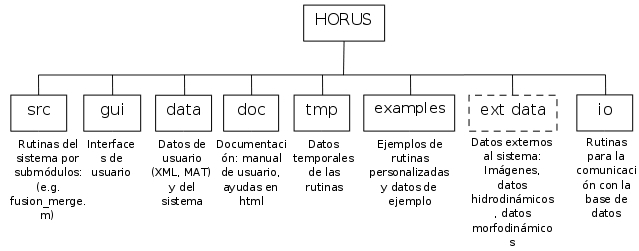
\includegraphics[width=1.0\linewidth]{img/dir}
  \caption{Esquema general del sistema de archivos de HORUS}
  \label{fig:dir}
\end{figure}

En el esquema se presentan todos los m�dulos del paquete que
contiene el sistema HORUS, los cuales se detallan a continuaci�n:

\begin{itemize}
\item M�dulo \emph{src}: Este m�dulo contiene las rutinas en MATLAB
  que llevan a cabo los procesos de HORUS, por ejemplo, rectificaci�n,
  fusi�n, entre otros.

\item M�dulo \emph{gui}: En este m�dulo se encuentran las interfaces
  de usuario, y se hace uso de las rutinas ubicadas en \emph{src} para
  la funcionalidad y de \emph{io} para la comunicaci�n con las bases
  de datos.

\item M�dulo \emph{data}: Contiene los datos de configuraci�n del
  sistema y del usuario, tales como las rutas de las im�genes,
  configuraciones, entre otros. Los datos contenidos en este m�dulo sirven
  como insumo para la funcionalidad de algunas rutinas y deben estar
  muy bien estructurados para facilidad de lectura y manipulaci�n.

\item M�dulo \emph{doc}: B�sicamente contiene los manuales t�cnicos y
  de usuario, as� como archivos en diferentes formatos (html, pdf,
  entre otros) que explican la funcionalidad de subm�dulos o rutinas.

\item M�dulo \emph{tmp}: Algunas rutinas requieren generar variables o
  archivos temporales, en este m�dulo se almacenan datos que pueden
  ser desechados posteriormente o no son vitales para el
  funcionamiento del sistema.

\item M�dulo \emph{examples}: Este m�dulo es una extensi�n de la
  documentaci�n donde se hacen demostraciones o ejemplos de alguna
  rutina, y datos de prueba.

\item M�dulo \emph{ext data}: Este m�dulo representa la base de datos
  de im�genes instant�neas, time exposure, variance o timestacks, de
  las zonas de estudio, as� como las series de tiempo, e informaci�n
  sobre la estaci�n. La l�nea punteada del recuadro indica que no se
  encuentra dentro del paquete de HORUS, pero hay comunicaci�n con
  este m�dulo.

\item M�dulo \emph{io}: Este m�dulo contiene rutinas espec�ficas para
  la comunicaci�n con una base de datos. Es el puente entre el m�dulo
  \emph{src} y \emph{gui} con la base de datos.
\end{itemize}

En la figura~\ref{fig:communication} se muestra un diagrama de
comunicaci�n entre los distintos m�dulos seg�n lo explicado
anteriormente. El dise�o del sistema est� constitu�do por tres
capas. La capa de m�s bajo nivel es la informaci�n que se almacena en
una base de datos relacional, la siguiente capa es un intermedio entre
la aplicaci�n y la base de datos, y est� constitu�da por las funciones
que consultan e insertan informaci�n en la base de datos desde las
funciones de usuario. La capa de m�s alto nivel, es la que contiene
las funciones que el usuario utiliza y las interfaces gr�ficas.

\begin{figure}[htbp] \centering
  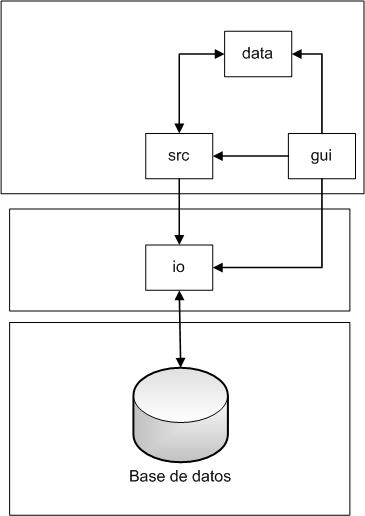
\includegraphics[width=0.5\linewidth]{img/communication}
  \caption{Diagrama de comunicaci�n entre los m�dulos}
  \label{fig:communication}
\end{figure}

El sistema HORUS consta de tres componentes b�sicamente, la captura,
que es donde se toman las im�genes y son enviadas a un servidor
central, el procesamiento, en el cual se manipulan las im�genes y se
extrae informaci�n de ellas, y la visualizaci�n en la web.

Este manual se enfoca en cada una de las componentes de HORUS,
principalmente en la etapa de procesamiento donde los procesos m�s
importantes son la rectificaci�n y la fusi�n.


\section{Base de datos}
\label{sec:dbdesign}

\subsection{Modelo Entidad--Relaci�n}

La base de datos de HORUS est� implementada en MySQL. En la
figura~\ref{fig:er} se muestra el modelo Entidad--Relaci�n (ER) donde
se detallan todas las entidades que componen la base de datos, los
atributos o caracter�sticas de cada una de estas entidades, y las
relaciones entre ellas. En este modelo se ven claramente todas las
componentes de la base de datos, las entidades son los recuadros, los
atributos son los �tems dentro de los recuadros, y las relaciones se
representan con las l�neas que unen cada par de entidades.

\begin{landscape}
  \begin{figure}[htbp]
    \centering
    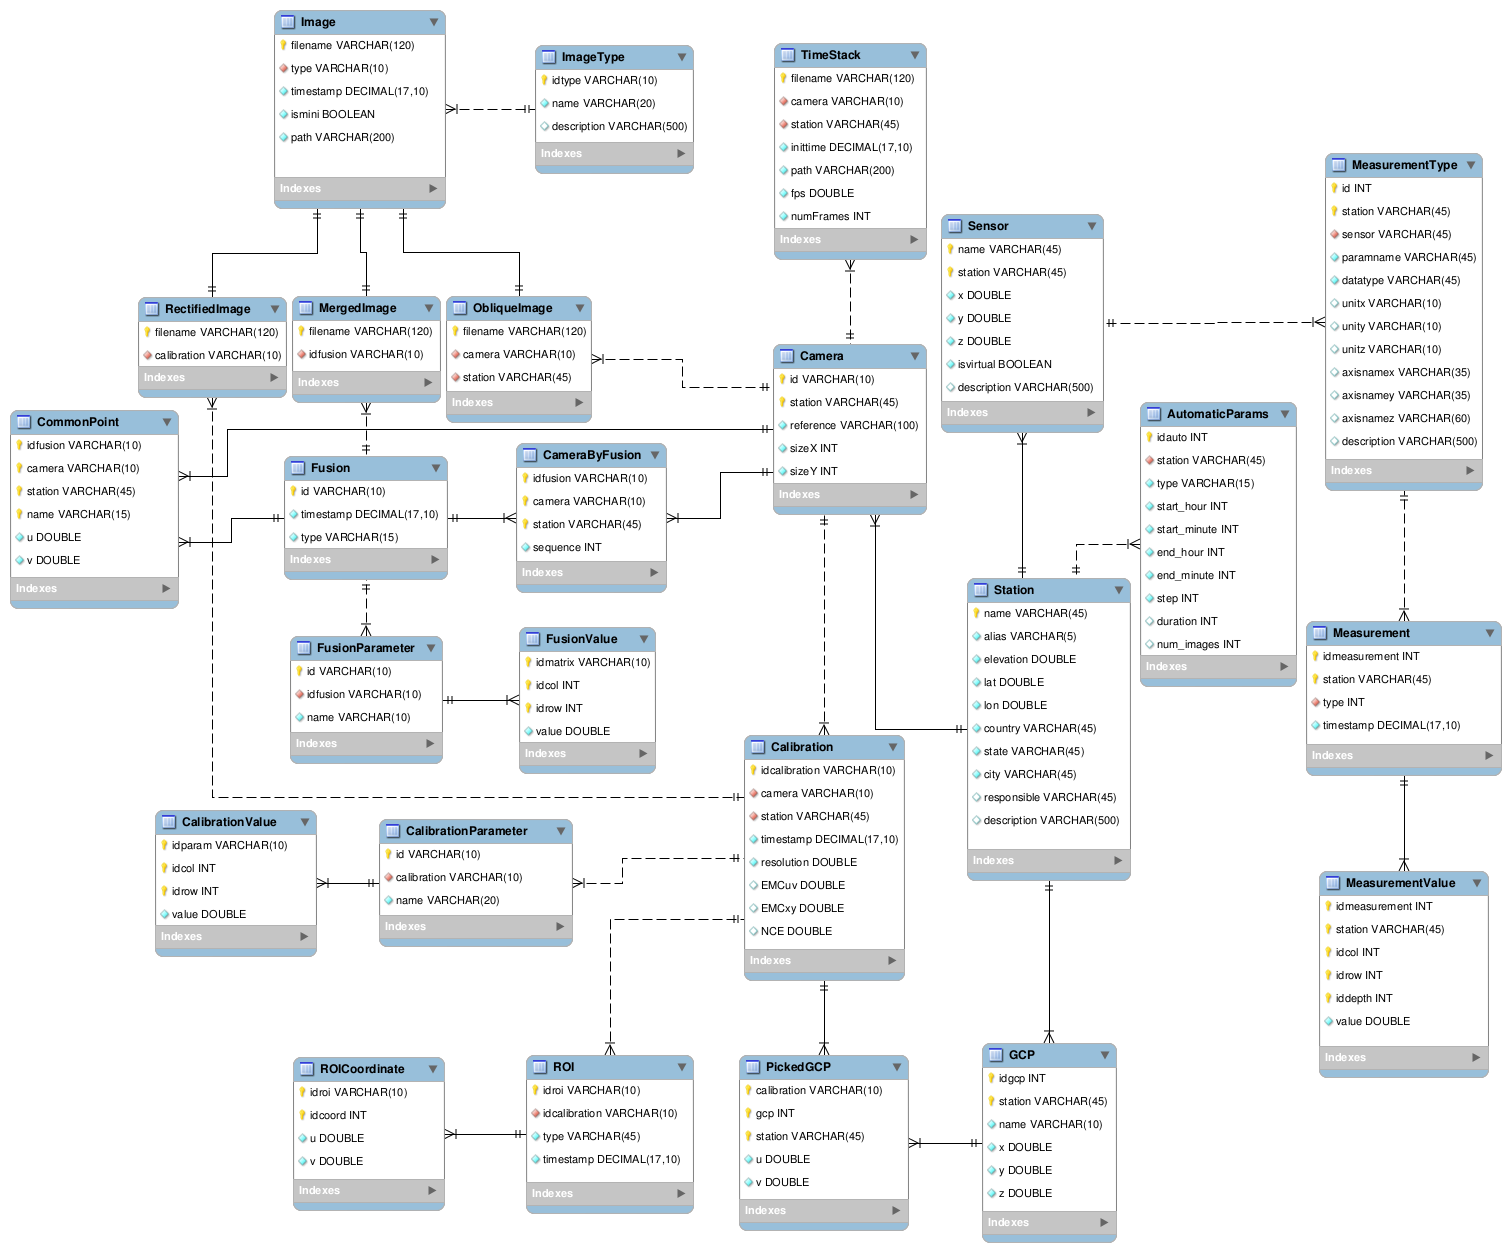
\includegraphics[width=0.7\linewidth]{img/ER_BD.png}
    \caption{Modelo ER de HORUS}
    \label{fig:er}
  \end{figure}
\end{landscape}


\newpage

\subsection{Entidades}

En esta secci�n se har� una descripci�n detallada de cada entidad que
aparece en el modelo ER de la figura~\ref{fig:er}. \textit{PK}
significa clave primaria, el cual es el atributo o conjunto de
atributos que identifican de manera �nica a una instancia de una
entidad con respecto a las otras instancias; \textit{FK} significa
clave for�nea, que es el atributo que referencia a una instancia de
otra entidad.

\subsubsection{Station}

Representa a la zona de estudio donde est�n instaladas las c�maras y
se hace la monitorizaci�n. Los atributos que contiene son:
\begin{itemize}
\item \emph{name (PK)}: Nombre de la estaci�n (e.g.\ Cartagena,
  Magdalena). Identifica de manera �nica al sitio.
\item \emph{alias}: Abreviatura del nombre de la estaci�n de m�ximo 5
  caracteres (e.g.\ CRTG).
\item \emph{elevation}: Elevaci�n sobre el nivel del mar en metros
  (e.g.\ $15$).
\item \emph{lat}: Latitud del sitio en grados (e.g.\ $43.46$).
\item \emph{lon}: Longitud del sitio en grados (e.g.\ $-3.77$).
\item \emph{country}: Pa�s donde se encuentra ubicada la estaci�n
  (e.g.\ Colombia).
\item \emph{state}: Estado o departamento donde se encuentra ubicada
  la estaci�n (e.g.\ Bol�var).
\item \emph{city}: Ciudad donde se encuentra ubicada la estaci�n
  (e.g.\ Cartagena).
\item \emph{responsible}: Nombre de la entidad o persona responsable
  de la estaci�n (e.g.\ Universidad de Cantabria).
\item \emph{description}: Descripci�n en palabras del sitio donde est�
  ubicada la estaci�n.
\end{itemize}
  
\subsubsection{Camera}
  
Esta entidad contiene informaci�n sobre las c�maras instaladas en la
estaci�n. Los atributos son:

\begin{itemize}
\item \emph{id (PK)}: Identificador de la c�mara en la estaci�n
  (e.g.\ C1, C2).
\item \emph{station (PK, FK)}: Nombre de la estaci�n, la cual junto
  con el identificador de la c�mara identifican de manera �nica a
  una c�mara en la base de datos. Es posible que en diferentes
  sitios haya c�maras con el mismo \emph{id}.
\item \emph{reference}: Marca o modelo de la c�mara (e.g.\ Marlin,
  Stingray, Sony webcam).
\item \emph{sizeX}: N�mero de p�xeles que el sensor puede capturar
  horizontalemte (e.g.\ $1024$).
\item \emph{sizeY}: N�mero de p�xeles que el sensor puede capturar
  verticalmente (e.g.\ $768$).
\end{itemize}
  
  
\subsubsection{ImageType}
  
Esta entidad representa los tipos de imagen que se generan en HORUS:
instant�neas (\textit{snapshot}), \textit{time exposure}
(\textit{timex}) y \textit{variance}, y sus caracter�sticas. Los
atributos son:

\begin{itemize}
\item \emph{idtype (PK)}: Clave que identifica de manera �nica a cada
  tipo en la base de datos. Se representa como el alias de la estaci�n
  m�s un autonum�rico (e.g.\ CRTG00023).
\item \emph{name}: Nombre del tipo. S�lo se permiten los valores:
  \textit{snap}, \textit{timex}, \textit{var}.
\item \emph{description}: Descripci�n en palabras del tipo de imagen.
\end{itemize}
  
\subsubsection{Image}

Esta entidad es un supertipo que representa a todas las im�genes que
se guardan en la base de datos (oblicuas, rectificadas,
fusionadas). No se almacenan las im�genes sino referencias a la
localizaci�n en un disco duro, o una direcci�n de red. Los atributos
de esta entidad son comunes a todos los tipos de im�genes y son los
siguientes:

\begin{itemize}
\item \emph{filename (PK)}: Nombre del archivo de la imagen\\ (e.g.\
  09.12.04.19.00.00.GMT.Cartagena.C1.Snap.1024X768.HORUS.jpg). Se
  supone que este nombre es �nico entre todas las im�genes presentes
  en la base de datos.
\item \emph{type (FK)}: Es una clave for�nea a la entidad
  \textit{ImageType}. Representa al tipo de la imagen (e.g.\
  \textit{snap}, \textit{timex}, \textit{var}).
\item \emph{timestamp}: El tiempo de la imagen (e.g.\ $734688.549$).
\item \emph{ismini}: Atributo booleano que indica si la imagen es o no
  una miniatura.
\item \emph{path}: Localizaci�n del archivo de la imagen (e.g.\
  /home/horus/images/).
\end{itemize}
  
\subsubsection{RectifiedImage}
  
Es un subtipo de \textit{Image}. Representa a las im�genes
rectificadas. Sus atributos son:

\begin{itemize}
\item \emph{filename (PK, FK)}: Clave for�nea a la entidad
  \textit{Image}.
\item \emph{calibration (FK)}: Clave for�nea a la entidad
  \textit{Calibration} y representa la calibraci�n utilizada para
  rectificar la imagen.
\end{itemize}
  
\subsubsection{MergedImage}

Es un subtipo de \textit{Image}. Representa a las im�genes fusionadas,
ya sean rectificadas u oblicuas (este tipo se encuentra en la entidad
\textit{Fusion}). Sus atributos son:

\begin{itemize}
\item \emph{filename (PK, FK)}: Clave for�nea a la entidad
  \textit{Image}.
\item \emph{idfusion (FK)}: Clave for�nea a la entidad
  \textit{Fusion}. Representa la geometr�a utilizada para fusionar varias
  im�genes.
\end{itemize}
  
\subsubsection{ObliqueImage}

Es un subtipo de Image. Representa a las im�genes oblicuas a las que
no se les ha aplicado ninguna transformaci�n. Sus atributos son:

\begin{itemize}
\item \emph{filename (PK, FK)}: Clave for�nea a la entidad
  \textit{Image}.
\item \emph{camera (FK)}: C�mara que gener� la imagen oblicua. Es
  clave for�nea a la entidad \textit{Camera} (e.g.\ C2).
\item \emph{station (FK)}: Estaci�n a la que corresponde la imagen. Es
  clave for�nea a la entidad \textit{Camera} (e.g.\ Cartagena).
\end{itemize}
  
\subsubsection{TimeStack}
  
Esta entidad representa a otro tipo de captura que se puede realizar
con las c�maras. Un \textit{timestack} se almacena como un v�deo que
contiene una secuencia de im�genes capturadas a una determinada
frecuencia, durante un tiempo determinado por el n�mero de im�genes
que se capturan. Al igual que las im�genes, no se almacena en la base
de datos el v�deo como tal sino una referencia a la localizaci�n donde
se encuentra almacenado, bien sea en un disco duro o en una direcci�n
de red. Sus atributos son:

\begin{itemize}
\item \emph{filename (PK)}: Nombre del archivo del timestack\\ (e.g.\
  11.03.24.12.00.00.GMT.CARTAGENA.C2.STACK.615.0.20X760.HORUS.jpg). Se
  supone que es �nico entre todos los \textit{timestacks} presentes en
  la base de datos.
\item \emph{camera (FK)}: C�mara que gener� el \textit{timestack}. Es
  clave for�nea a la entidad \textit{Camera}.
\item \emph{station (FK)}: Estaci�n donde se captur� el
  \textit{timestack}. Es clave for�nea a la entidad \textit{Camera}.
\item \emph{inittime}: Tiempo de inicio de la captura.

\item \emph{path}: Localizaci�n del archivo del \textit{timestack}
  (e.g.\ /home/horus/stacks/).
\item \emph{fps}: Frecuencia o \textit{framerate} en Hertz. Es el
  n�mero de im�genes que se capturan por segundo (e.g.\ $2$).
\item \emph{numFrames}: N�mero de frames que se capturan a la
  frecuencia dada (e.g.\ $1200$).
\end{itemize}
  
\subsubsection{GCP}

Esta entidad representa a los puntos de control georeferenciados para
un sitio que sirven como punto de partida para los modelos de
optimizaci�n utilizados para rectificar y fusionar im�genes. Sus
atributos son:

\begin{itemize}
\item \emph{idgcp (PK)}: Es un identificador de cada punto en un
  sitio. Es posible que haya dos GCPs en estaciones distintas con el
  mismo identificador.
\item \emph{station (PK)}: Nombre de la estaci�n a la que corresponde
  un GCP\@. Junto con el \emph{idgcp} identifican de manera �nica un
  GCP en la base de datos.
\item \emph{name}: Nombre que se le da al GCP para facilidad de
  representaci�n (e.g.\ GCP001).
\item \emph{x, y, z}: Coordenada georreferenciada del GCP (e.g.\ $500$,
  $1000$, $0$).
\end{itemize}

\subsubsection{Calibration}

Esta entidad representa una calibraci�n de una c�mara en una fecha en
particular mediante un modelo como el \textit{DLT} o
\textit{Pinhole}. Pueden haber varias calibraciones en el tiempo
debido a cambios leves en la posici�n de las c�maras. Sus atributos
son:

\begin{itemize}
\item \emph{idcalibration (PK)}: Clave que identifica de manera �nica
  a cada calibraci�n en la base de datos. Se representa como el alias
  de la estaci�n m�s un autonum�rico (e.g.\ CRTG00023).
\item \emph{camera (FK)}: C�mara en la que se hace la calibraci�n. Es
  clave for�nea a la entidad \textit{Camera}.
\item \emph{station (FK)}: Estaci�n donde se hace la calibraci�n. Es
  clave for�nea a la entidad \textit{Camera}.
\item \emph{timestamp}: Fecha en la que se hizo la calibraci�n.
\item \emph{resolution}: Resoluci�n de la rectificaci�n (e.g. $0.5$).
\item \emph{EMCuv}: Error cuadr�tico medio del modelo en p�xeles.
\item \emph{EMCxy}: Error cuadr�tico medio de las proyecciones en
  metros.
\item \emph{NCE}: Error de calibraci�n normalizado.
    
\end{itemize}
  
\subsubsection{PickedGCP}

Para cada calibraci�n, hay un subconjunto de los GCP de una estaci�n
que son escogidos como insumo para el modelo de optimizaci�n. Esta
entidad representa cu�les GCP que corresponde a una estaci�n est�n
relacionados con una calibraci�n en particular y la relaci�n entre sus
coordenadas $(x, y, z)$ y las coordenadas $(u, v)$ marcadas por el
usuario. Los atributos son:

\begin{itemize}
\item \emph{calibration (PK, FK)}: Es la calibraci�n a la que est�n
  relacionados los puntos. Es clave for�nea a la entidad
  \textit{Calibration}.
\item \emph{gcp (PK, FK)}: Es el n�mero del punto de control que se
  relaciona. Es clave for�nea a la entidad \textit{GCP}.
\item \emph{station (PK, FK)}: Es la estaci�n a la que corresponde el
  GCP\@. Es clave for�nea a la entidad \textit{GCP}.
\item \emph{u, v}: Posici�n en p�xeles en la c�mara de cada punto de
  control transformado mediante los par�metros de la calibraci�n a la
  que est� relacionado (e.g.\ $300$, $200$).
\end{itemize}
  
\subsubsection{CalibrationParameter}

Esta entidad representa los par�metros que pueden ser matrices o
escalares de una calibraci�n. En realidad no se almacena el valor del
par�metro, sino su informaci�n. Los atributos son:

\begin{itemize}
\item \emph{id (PK)}: Clave que identifica de manera �nica a cada
  par�metro en la base de datos. Se representa como el alias de la
  estaci�n m�s un autonum�rico (e.g.\ CRTG00023).
\item \emph{calibration (FK)}: Es la clave for�nea o la referencia a
  la calibraci�n que est� relacionada con el par�metro.
\item \emph{name}: Es el nombre del par�metro, es �til para saber
  exactamente a qu� matriz o valor escalar se refiere el par�metro
  (e.g.\ H, P, K).
\end{itemize}
  
\subsubsection{CalibrationValue}

Esta entidad representa la matriz donde se almacena el valor del
par�metro de una calibraci�n. La manera de representar a una matriz, ya
que el gestor de base de datos no posee un tipo de datos matriz, es
como un conjunto de filas que corresponden a cada elemento de la
matriz y cada una se identifica mediante un identificador de columna,
de fila, y valor. Los atributos son:

\begin{itemize}
\item \emph{idparam (PK, FK)}: Es la clave for�nea o referencia a la
  entidad \textit{CalibrationParameter}, y representa el par�metro al
  que est� relacionado.
\item \emph{idcol (PK)}: Identificador de la columna de la matriz (los
  �ndices comienzan en 1).
\item \emph{idrow (PK)}: Identificador de la fila de la matriz (los
  �ndices comienzan en 1).
\item \emph{value}: Valor escalar de cada elemento de la matriz.
\end{itemize}
  
\subsubsection{Fusion}

Esta entidad representa los par�metros que son espec�ficos para
fusionar im�genes, bien sea rectificadas u oblicuas. Los atributos
son:

\begin{itemize}
\item \emph{id (PK)}: Clave que identifica de manera �nica a los datos
  de la fusi�n en la base de datos. Se representa como el alias de la
  estaci�n m�s un autonum�rico (e.g.\ CRTG00023).
\item \emph{timestamp}: Tiempo en el que se crearon los par�metros para
  la fusi�n. Sirve para encontrar la fusi�n m�s cercana a una fecha
  especificada.
\item \emph{type}: Es el tipo de im�genes que se va a fusionar. Los
  valores que puede tomar son: \textit{rectified} y \textit{oblique}.
\end{itemize}
  

\subsubsection{FusionParameter}

Al igual que la entidad \textit{CalibrationParameter}, representa una
matriz o escalar de la calibraci�n para una fusi�n o la transformaci�n
af�n entre dos im�genes. No se almacena aqu� el valor. Los atributos
son:

\begin{itemize}
\item \emph{id (PK)}: Clave que identifica de manera �nica a una
  matriz de fusi�n en la base de datos. Se representa como el alias de
  la estaci�n m�s un autonum�rico (e.g.\ CRTG00023).
\item \emph{idfusion (FK)}: Clave for�nea o referencia a la entidad
  \textit{Fusion} e identifica la fusi�n a la que corresponde la
  matriz.
\item \emph{name}: Es el nombre de la matriz (e.g.\ H12, H23).
\end{itemize}


\subsubsection{FusionValue}

Esta entidad representa la matriz donde se almacena el valor del
par�metro de una fusi�n. La manera de representar a una matriz, ya que
el gestor de base de datos no posee un tipo de datos matriz, es como
un conjunto de filas que corresponden a cada elemento de la matriz y
cada una se identifica mediante un identificador de columna, de fila,
y valor. Los atributos son:

\begin{itemize}
\item \emph{idmatrix (PK, FK)}: Es la clave for�nea o referencia a la
  entidad \textit{FusionParameter}, y representa la matriz al que est�
  relacionado.
\item \emph{idcol (PK)}: Identificador de la columna de la matriz (los
  �ndices comienzan en 1).
\item \emph{idrow (PK)}: Identificador de la fila de la matriz (los
  �ndices comienzan en 1).
\item \emph{value}: Valor escalar de cada elemento de la matriz.
\end{itemize}
  
\subsubsection{CameraByFusion}

Para realizar una fusi�n es necesario saber cu�les c�maras est�n
involucradas y en qu� orden de la fusi�n va cada c�mara. Para
representar esto se utiliza esta entidad que almacena para cada fusi�n
las c�maras relacionadas y el orden de cada una. Los atributos son:

\begin{itemize}
\item \emph{idfusion (PK, FK)}: Es la clave for�nea o referencia a la
  fusi�n a la que se le quieren relacionar las c�maras.
\item \emph{camera (PK, FK)}: Es el identificador de la c�mara que se
  quiere incluir. Es clave for�nea a la entidad \textit{Camera}.
\item \emph{station (PK, FK)}: Es la estaci�n en la que se realiza el
  proceso. Es clave for�nea a la entidad \textit{Camera}.
\item \emph{sequence}: El orden en el que la c�mara act�a en la fusi�n
  (comenzando en $1$).
\end{itemize}

\subsubsection{Common Point}

Para cada fusi�n, hay un conjunto de puntos comunes entre cada par de
c�maras de una estaci�n que son escogidos como insumo para el modelo
de optimizaci�n. Esta entidad representa estos puntos, asociados a una
c�mara de la estaci�n relacionados con una fusi�n en particular. Los
atributos son:

\begin{itemize}
\item \emph{idfusion (PK, FK)}: Es la fusi�n a la que est�n
  relacionados los puntos. Es clave for�nea a la entidad
  \textit{Fusion}.
\item \emph{camera (PK, FK)}: Es el ID de la c�mara a la que est�
  asignado cada punto. Es clave for�nea a la entidad \textit{Camera}.
\item \emph{station (PK, FK)}: Es la estaci�n a la que corresponde el
  punto. Es clave for�nea a la entidad \textit{Camera}.
\item \emph{name (PK)}: Nombre asignado al punto en com�n. Este nombre
  es compartido con el otro punto correspondiente en la otra c�mara.
\item \emph{u, v}: Posici�n en p�xeles en la c�mara de cada punto
  com�n (e.g.\ $300$, $200$).
\end{itemize}
  
\subsubsection{ROI}

En HORUS los ROIs tienen diversas aplicaciones, por ejemplo, para
definir el �rea de la imagen que se captura en un \textit{timestack},
el �rea que se quiere rectificar o fusionar en una imagen, entre
otros. La manera de representar un ROI es mediante un conjunto de
coordenadas $(u, v)$ en p�xeles que representan los v�rtices del
pol�gono. La entidad ROI representa esto, aunque no almacena las
coordenadas como tal. Sus atributos son los siguientes:

\begin{itemize}
\item \emph{idroi (PK)}: Clave que identifica de manera �nica a un ROI
  en la base de datos. Se representa como el alias de la estaci�n m�s
  un autonum�rico (e.g.\ CRTG00023).
\item \emph{idcalibration (FK)}: Es la clave for�nea a la entidad
  \textit{Calibration} y representa la calibraci�n a la que est�
  relacionado el ROI.
\item \emph{type}: Es el tipo de ROI o el tipo de aplicaci�n de un ROI
  en particular. Los valores que puede tomar son: \textit{fusion},
  \textit{rect}, \textit{stack}, \textit{user}.
\item \emph{timestamp}: Fecha en la que se cre� el ROI\@.
\end{itemize}
  
\subsubsection{ROICoordinate}

Esta entidad representa las coordenadas de los v�rtices del pol�gono
que definen un ROI en particular. Los atributos son:

\begin{itemize}
\item \emph{idroi (PK, FK)}: Es la clave for�nea al ROI al que
  pertenece cada coordenada.
\item \emph{idcoord (PK)}: Es un n�mero que identifica cada
  coordenada. Pueden haber n�meros iguales en distintos ROIs. El
  pol�gono se forma uniendo mediante l�neas rectas dos puntos con
  \textit{idcoord} consecutivos. El �ltimo se une con el primero.
\item \emph{u, v}: El valor de la coordenada en p�xeles.
\end{itemize}
  
\subsubsection{Measurement}

Esta entidad representa las series de tiempo de medici�n de
diversas variables que es interesante mantener almacenadas, por
ejemplo, altura de ola, marea astron�mica, densidad de usuarios,
posici�n de la l�nea de costa, entre otros. En esta entidad no se
guarda el valor como tal de la medici�n ya que puede ser un
escalar, una matriz de dos o incluso tres dimensiones. Los atributos
son:

\begin{itemize}
\item \emph{idmeasurement (PK)}: Autonum�rico que identifica de manera
  �nica a una medici�n en la base de datos.
\item \emph{station}: Nombre de la estaci�n a la que est� relacionado
  (e.g.\ Cartagena, Magdalena).
\item \emph{type (FK)}: Tipo de medici�n. Es clave for�nea a la
  entidad MeasurementType.
\item \emph{timestamp}: Tiempo de la medici�n.
\end{itemize}
  
\subsubsection{MeasurementType}

Esta entidad representa el tipo de una medici�n en particular. Los
atributos son:

\begin{itemize}
\item \emph{id (PK)}: Autonum�rico que identifica a un tipo de
  medici�n en la base de datos.
\item \emph{station (PK FK)}: Estaci�n a la que pertenece la
  medici�n.
\item \emph{sensor (FK)}: Es la clave for�nea a la entidad
  \textit{Sensor} y representa el sensor con el que se miden las
  mediciones de un tipo en particular.
\item \emph{paramname}: Es el nombre del par�metro (e.g.\ Hs, T).
\item \emph{datatype}: Es el tipo de dato que se esta guardando. Los
  valores que puede tomar son: \textit{series}, \textit{matrix}.

\item \emph{unitx}: Unidad de medida del eje x en el tipo de
  medici�n (e.g.\ m, �C, m/s).
\item \emph{unity}: Unidad de medida del eje y en el tipo de
  medici�n (e.g.\ m, �C, m/s).
\item \emph{unitz}: Unidad de medida del eje z en el tipo de
  medici�n (e.g.\ m, �C, m/s).
\item \emph{axisnamex}: Es el mensaje que se colocar�a en el eje x de
  una gr�fica.
\item \emph{axisnamey}: Es el mensaje que se colocar�a en el eje y de
  una gr�fica.
\item \emph{axisnamez}: Es el mensaje que se colocar�a de titulo de
  una gr�fica.
\item \emph{description}: Descripci�n verbal del tipo de medici�n.
\end{itemize}
  
\subsubsection{MeasurementValue}

Esta entidad representa el valor de una medici�n. Una medici�n se
puede representar como un valor escalar, una matriz de dos o tres
dimensiones. Cada valor de la matriz se identifica por la medici�n
a la que corresponde, un identificador de fila, columna y
profundidad. Los atributos son:

\begin{itemize}
\item \emph{idmeasurement (PK, FK)}: Clave for�nea o referencia a la
  medici�n a la que corresponde cada elemento de la matriz.
\item \emph{station (PK FK)}: Estaci�n a la que pertenece la
  medici�n.
\item \emph{idcol (PK)}: Identificador de la columna de la matriz (los
  �ndices comienzan en 1).
\item \emph{idrow (PK)}: Identificador de la fila de la matriz (los
  �ndices comienzan en 1).
\item \emph{iddepth (PK)}: Identificador de la profundidad (tercera
  dimensi�n) de la matriz (los �ndices comienzan en 1).
\item \emph{value}: Valor del elemento de la matriz.
\end{itemize}

  
\subsubsection{Sensor}

Esta entidad representa la informaci�n de un sensor con el que se mide
alg�n tipo de medici�n (e.g.\@ Boya es un sensor para medir altura
de ola, per�odo de la ola, entre otros). Los atributos son los
siguientes:

\begin{itemize}
\item \emph{name}: Nombre �nico del sensor (e.g.\ DCX22).
\item \emph{station (PK FK)}: Nombre de la estaci�n a la que est�
  relacionado el sensor. Es clave for�nea a la entidad
  \textit{Station}.
\item \emph{x, y, z}: Coordenada georreferenciada del sensor (e.g.\
  $500$, $1000$, $0$).
\item \emph{description}: Descripci�n verbal del sensor.
\end{itemize}

\subsubsection{AutomaticParams}

Esta entidad contiene la configuraci�n de los tiempos de los autom�ticos para
una estaci�n. Con estos tiempos, es posible sincronizar procesos como
la rectificaci�n y fusi�n autom�ticas. Los atributos que contiene son:

\begin{itemize}
\item \emph{idauto (PK)}: Autonum�rico que identifica de manera
  �nica a un autom�tico en la base de datos.
\item \emph{station (FK)}: Estaci�n a la que pertenece la captura.
\item \emph{type}: Tipo de la captura, puede ser \textit{image},
  \textit{stack}, \textit{transfer} o \textit{process}.
\item \emph{start\_hour}: Hora de inicio de la captura en el d�a
  (e.g.\ $06$).
\item \emph{start\_minute}: Minuto de inicio de la captura en una hora
  (e.g.\ $30$).
\item \emph{end\_hour}: Hora de finalizaci�n de la captura en el d�a
  (e.g.\ $18$).
\item \emph{end\_minute}: Minuto de finalizaci�n de la captura en una
  hora (e.g.\ $30$).
\item \emph{step}: Tiempo de espera entre captura y captura, en
  minutos.
\item \emph{duration}: Tiempo de duraci�n de la captura.
\item \emph{num\_images}: Numero de im�genes capturadas.
\end{itemize}


\chapter{Instalaci�n}
\label{chap:installation}

\section{Instalaci�n B�sica}

El sistema HORUS fue dise�ado para trabajar con la versi�n de
\textregistered MATLAB R2011b o superior y requiere el Toolbox de
Procesamiento de Im�genes y el de Bases de datos. Si su instalaci�n de
\textregistered MATLAB cumple los requisitos b�sicos puede poner los
archivos del sistema HORUS en cualquier directorio (e.g.\@
\verb!/home/horus!). Los archivos del sistema HORUS inicialmente est�n
comprimidos en \texttt{horus.zip}, el primer paso es descomprimirlos
en el directorio de preferencia.  El computador donde se ejecute el
sistema HORUS debe contar m�nimo con 2GB de memoria RAM. Si la captura
y el procesamiento de las im�genes se hacen en m�quinas diferentes, es
necesario tener un servidor SSH en el computador donde funcione la
captura para enviar la informaci�n al computador de procesamiento. Si
se tiene un sitio web para enviar informaci�n (e.g.\
\url{www.horusvideo.com}), el sitio debe tener servicio de FTP para
recibir la informaci�n desde el computador de procesamiento.

Para visualizar todas interfaces gr�ficas apropiadamente, se
recomienda una resoluci�n de pantalla de m�nimo $1200 \times 800$.

\section{Base de Datos}
\label{sec:db}
El sistema HORUS fue dise�ado para trabajar con una base de datos
relacional en MySQL. Antes de trabajar con HORUS es necesario
configurar la base de datos ya que en �sta va a estar almacenada toda
la informaci�n que necesita HORUS para trabajar. Es posible trabajar
con el sistema HORUS a partir de una base de datos existente a la que
se pueda acceder, bien sea mediante una red local o por
Internet. Tambi�n es posible configurar una nueva base de datos desde
cero.

Este paso se puede realizar utilizando la interfaz gr�fica \emph{Setup
  database} de la interfaz principal (ver Cap�tulo~\ref{chap:gui}), o
realizando los pasos manualmente. Se recomienda utilizar la interfaz
gr�fica mientras sea posible, se deja la configuraci�n manual para
usuarios avanzados.

\subsection{Configuraci�n mediante la interfaz gr�fica \emph{Setup
    database}}

La interfaz \emph{Setup database} se puede ejecutar presionando el
bot�n correspondiente en la interfaz principal de HORUS o escribiendo
el comando \verb!gui_configure_database! en la l�nea de comandos de
Matlab. En la figura~\ref{fig:setupdb} se muestra la interfaz.

\begin{figure}[htbp!]
  \centering
%  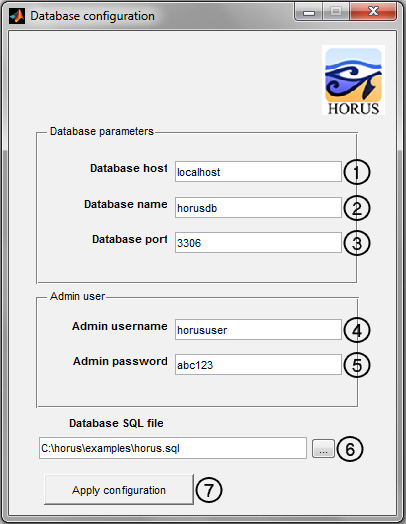
\includegraphics[width=0.4\textwidth]{img/setupdb}
  \caption{Interfaz para configuraci�n inicial de la base de datos}
  \label{fig:setupdb}
\end{figure}

Las componentes numeradas en la interfaz se explican a continuaci�n (los
campos con * son obligatorios):

\begin{enumerate}
\item Database host: Es la direcci�n IP o nombre del host donde se
  encuentra el servidor MySQL.
\item Database name: Todas las bases de datos deben tener un
  nombre. En este campo se especifica este nombre, el cual es
  diferente para las bases de datos presentes en el servidor.
\item Database port: Es el puerto del servidor MySQL, a menos que el
  administrador del servidor haya decidido seleccionar uno diferente,
  el puerto por defecto es 3306.
\item Admin username: Es el nombre de usuario del administrador de la
  base de datos de HORUS. Este usuario es el encargado de realizar las
  modificaciones principales en la base de datos y de crear nuevos
  usuarios con privilegios limitados.
\item Admin password: Es la contrase�a del usuario administrador de la
  base de datos.
\item Database SQL file: Se debe seleccionar el archivo en formato SQL
  con la especificaci�n del esquema relacional de HORUS. Este archivo
  se provee junto con el software en \verb!examples/horus.sql!. Sin
  embargo, es posible definir otro esquema siempre y cuando cumpla con
  las especificaciones de la base de datos, con datos insertados en
  las tablas de la base de datos.
\item Apply configuration: Este bot�n ejecuta la configuraci�n creando
  el esquema de la base de datos en el servidor MySQL y el usuario
  administrador. Desde aqu� es posible insertar informaci�n en la base
  de datos utilizando el usuario administrador.
\end{enumerate}

\subsection{Configuraci�n manual}

\subsubsection{Configuraci�n del cliente de MySQL}

Para establecer la conexi�n a una base de datos MySQL existente, es
necesario configurar MATLAB para trabajar como cliente. En MATLAB
existe una variable de entorno llamada \verb!$matlabroot! que
representa el directorio de instalaci�n de MATLAB (e.g.\@
\verb!C:\MATLAB\R2011b!), y la utilizaremos para localizar los
archivos propios de MATLAB. Los pasos para lograr esto son los
siguientes:

\begin{enumerate}
\item Asegurarse que el \textit{Database Toolbox} de MATLAB est�
  instalado junto con MATLAB.
\item Descargar el \textit{plugin} para conexi�n con MySQL. En el
  momento de escribir este manual, este plugin se puede descargar
  desde \texttt{\url{http://dev.mysql.com/downloads/connector/j}}
  seleccionando el sistema operativo correspondiente.
\item Descomprimir el archivo.
\item En el directorio descomprimido hay un archivo llamado\\
  \verb!mysql-connector-java-<version>-bin.jar! (donde
  \verb!<version>! es la versi�n del plugin). Copiar este archivo al
  directorio \verb!$matlabroot/java/jarext/!.
\item Agregar al archivo
  \verb!$matlabroot/toolbox/local/classpath.txt! la l�nea\\
  \verb!$matlabroot/java/jarext/mysql-connector-java-<version>-bin.jar!\\
  (donde \verb!<version>! es la versi�n del plugin). En el sistema operativo 
  Windows 7 este archivo no se puede editar por la ubicaci�n en la que se 
  encuentra por esta raz�n se debe copiar este archivo en otra carpeta como 
  por ejemplo en el escritorio, hacer el cambio y reemplazar el archivo anterior. 
  Por �ltimo si MATLAB se encontraba ejecut�ndose para que los cambios funcionen 
  se debe de cerrar y volver a abrir.
\end{enumerate}

Ahora, es posible que las funciones de MATLAB hagan conexi�n con una
base de datos existente. Se debe establecer la direcci�n de conexi�n
del servidor de la base de datos.

\subsubsection{Configuraci�n de una nueva base de datos}

Las funciones de HORUS utilizan una base de datos cuya estructura se
detalla en el cap�tulo~\ref{sec:dbdesign}. Para crear una nueva base
de datos con esta estructura se deben seguir los siguientes pasos (si
ya existe una instalaci�n anterior de MySQL, no es necesario volver a
instalarlo ya que puede generar problemas debido a cuentas de usuario
anteriores):

\begin{enumerate}
\item Instalar el servidor de MySQL, que se puede descargar desde
  \texttt{\url{http://dev.mysql.com/downloads/mysql/}}. En los pasos
  de la instalaci�n se deben tener en cuenta los siguientes aspectos
  en Windows:
  \begin{itemize}
  \item Seleccionar instalaci�n \emph{T�pica}.
  \item Seleccionar la opci�n ``Instalar como \emph{Servicio del
      sistema}''.
  \item Seleccionar la opci�n ``Incluir la ruta de la instalaci�n en
    el \verb!PATH! del sistema''.
  \item Reiniciar PC.
  \item Por defecto, existe un usuario administrador del servidor. Se
    debe especificar la contrase�a de este usuario (\verb!root!).
  \end{itemize}

  Si se quiere instalar el servidor de MySQL en Linux, es suficiente
  con instalarlo desde el repositorio de paquetes de la distribuci�n
  espec�fica.
\item Inicialmente, el �nico usuario en MySQL es el usuario
  \texttt{root}. En la l�nea de comandos acceder a MySQL mediante el
  comando:

  \begin{flushleft}
    \verb!mysql -h <direcci�n> -u root -p!
  \end{flushleft}
  
  Donde \verb!<direcci�n>! es la direcci�n IP del servidor MySQL
  (\verb!localhost! si es local).  Crear la base de datos mediante el
  comando:

  \begin{flushleft}
    \verb!mysql> CREATE DATABASE horus!;
  \end{flushleft}

  El nombre de la base de datos en este caso es \texttt{horus}, sin
  embargo, este nombre es arbitrario, puede ser cualquiera.

\item Se deben crear los usuarios administradores de la base de datos,
  que tendr�n acceso a la base de datos y sus permisos. Supongamos que
  queremos crear el usuario \textit{horususer} que tendr� todos los
  privilegios para manipular la base de datos. Los comandos para crear
  el usuario con todos los privilegios, son los siguientes:

  \begin{flushleft}
    \verb!mysql> GRANT ALL PRIVILEGES ON horus.* TO 'horususer'@'%'!\\
    \verb!  IDENTIFIED BY '<password>' WITH GRANT OPTION;!

    \verb!mysql> FLUSH PRIVILEGES;!

    \verb!mysql> QUIT;!
  \end{flushleft}

  Donde \verb!<password>! es la contrase�a del usuario.

\item Ya hemos creado un usuario y un esquema de la base de datos,
  ahora debemos crear la estructura de la base de datos. El archivo
  \texttt{horus.sql} del directorio \verb!examples! en el paquete de
  HORUS contiene el c�digo SQL para crear la estructura de la base de
  datos. Para ejecutar este c�digo se ingresa el siguiente comando
  desde la l�nea de comandos del sistema (suponiendo que est� en el
  directorio \verb!examples!):

  \begin{flushleft}
    \verb!mysql -h <direcci�n> -u horususer -p horus < horus.sql!
  \end{flushleft}

  Donde \verb!<direcci�n>! es la direcci�n IP del servidor MySQL
  (\verb!localhost! si es local).

  \emph{Precauci�n}: Al ejecutar este comando, toda la informaci�n
  previa guardada en la base de datos \textit{horus} ser� eliminada
  (en caso de una instalaci�n anterior).

\end{enumerate}

Opcionalmente, si se dispone de un archivo de inserciones en SQL de la
nueva informaci�n, podemos utilizar este archivo para alimentar la
base de datos, en caso contrario, es necesario insertar los datos
manualmente, mediante las interfaces gr�ficas descritas en el
cap�tulo~\ref{chap:gui}. Supongamos que tenemos el archivo
\verb!insert.sql! que contiene la informaci�n nueva de la base de
datos. Para insertar toda la informaci�n en la base de datos, se
ejecuta el siguiente comando desde la l�nea de comandos del sistema
(suponiendo que est� en el mismo directorio donde est� el archivo
\verb!insert.sql!):

  \begin{flushleft}
    \verb!mysql -h <direcci�n> -u horususer -p horus < insert.sql!
  \end{flushleft}

Cuando se quiere utilizar manualmente alguna de las funciones que se
comunican con la base de datos, del directorio \texttt{io}, es
necesario crear la conexi�n con la base de datos de antemano. El
siguiente c�digo sirve para crear una nueva conexi�n:

\begin{verbatim}
try
    conn = connection_db();
catch e
    disp(e.message)
end
\end{verbatim}

Si no se ha iniciado una sesi�n en HORUS, se solicitan los datos de
\textit{login}. Es importante que luego de utilizar alguna funci�n de
\texttt{io}, se cierre la conexi�n con la base de datos. Esto se puede
hacer as�:

\begin{verbatim}
close(conn)
\end{verbatim}

\chapter{GUI}
\label{chap:gui}

Las secciones que siguen contienen una descripci�n de las interfaces
gr�ficas usadas en HORUS para llevar a cabo los diferentes procesos
como configuraci�n de la captura, procesamiento de las im�genes y
almacenamiento en la base de datos. Estas interfaces se encuentran en
el directorio \verb!gui! de HORUS y para poder ejecutarlas, se debe
agregar la ruta\footnote{Es posible que al copiar y pegar este
  comando, las \texttt{'} no sean las mismas que MATLAB utiliza}:

\begin{verbatim}
>> addpath('gui')
\end{verbatim}

Cuando se ejecuta por primera vez alguna de las interfaces que se
detallan a continuaci�n, se despliega una interfaz para hacer el
\textit{login} en la base de datos, con el usuario creado previamente
en la instalaci�n. En la figura~\ref{fig:login} se muestra la ventana
de \textit{login}. Este \textit{login} solamente se hace una vez
mientras dura la sesi�n de usuario. Cuando se cierra alguna interfaz,
se pregunta al usuario si desea cerrar la sesi�n o no.

\begin{figure}[htbp!]
  \centering
  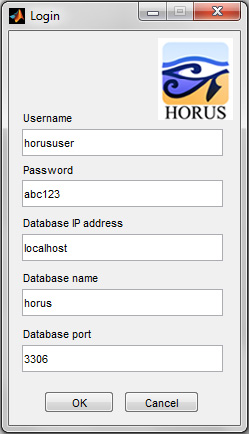
\includegraphics[width=0.4\textwidth]{img/login}
  \caption{Interfaz para ingresar los datos de usuario para el login}
  \label{fig:login}
\end{figure}

Las componentes numeradas de la interfaz son:

\begin{enumerate}
\item Nombre de usuario de la base de datos.
\item Contrase�a (no se muestran los caracteres mientras se digitan).
\item Nombre o direcci�n del servidor donde se encuentra alojada la
  base de datos (\texttt{localhost} si es local).
\item Nombre del esquema de la base de datos (por defecto es
  \texttt{horus}).
\item Puerto de la base de datos (por defecto es \texttt{3306}).
\end{enumerate}

\emph{NOTA}: Es posible que cuando se est� utilizando una interfaz
gr�fica, la conexi�n con la base de datos caduque, por lo que en ese
caso, hay que cerrar y abrir nuevamente la interfaz con el fin de
renovar la conexi�n.

El manejo de sesiones en HORUS no tiene que ver con la conexi�n a la
base de datos y la vigencia de �sta, sino con la informaci�n del
archivo \texttt{userinfo.dat} del directorio \texttt{tmp}. Este
archivo de texto plano contiene el nombre de usuario de la base de
datos (\textit{user}), la contrase�a encriptada (\textit{password}),
la direcci�n del servidor de la base de datos (\textit{host}), el
puerto (\textit{port}) y el nombre de la base de datos
(\textit{dbname}). Cuando un usuario se loguea, debe ingresar toda la
informaci�n mencionada para la conexi�n a la base de datos, y se crea
el archivo \texttt{userinfo.dat}. Cuando, por ejemplo, el usuario
cierra una interfaz gr�fica, el sistema le pregunta al usuario si
desea cerrar la sesi�n, en caso afirmativo, el archivo
\texttt{userinfo.dat} es borrado, y en caso negativo no se hace nada.
En conclusi�n, mientras el archivo \texttt{userinfo.dat} exista, hay
una sesi�n de HORUS abierta, y se cierra cuando el archivo es borrado.

\section{DB Editor}

El sistema HORUS cuenta con una base de datos en la cual se ingresa
toda la informaci�n generada necesaria para el correcto funcionamiento
del sistema (ver secci�n~\ref{sec:dbdesign}). Con esta interfaz se
puede insertar, actualizar o eliminar la informaci�n de una estaci�n,
una c�mara, un GCP, un sensor o un tipo de medici�n (los cuales son
los par�metros que mide un sensor). Al abrir la interfaz se muestra la
opci�n de insertar una nueva estaci�n a la base de datos de HORUS. Si
se desea, con el men� de la parte superior se puede cambiar de opci�n
para actualizar o insertar estaciones, c�maras, GCPs, sensores y tipos
de mediciones. A continuaci�n se explica cada una de las opciones
de la interfaz.

El comando para ejecutar esta interfaz es: \texttt{gui\_db\_editor}.

\subsection{Estaci�n}

En la figura~\ref{fig:station} se muestra la opci�n de insertar una
nueva estaci�n en la base de datos, y en la figura~\ref{fig:station2}
la opci�n de actualizar o eliminar una estaci�n existente.

\begin{figure}[htbp!]
  \centering
  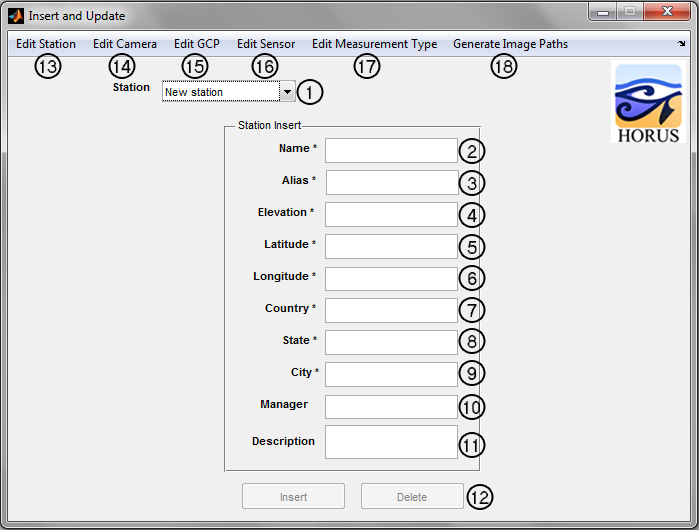
\includegraphics[width=0.6\textwidth]{img/station}
  \caption{Interfaz para insertar una nueva estaci�n}
  \label{fig:station}
\end{figure}

\begin{figure}[htbp!]
  \centering
  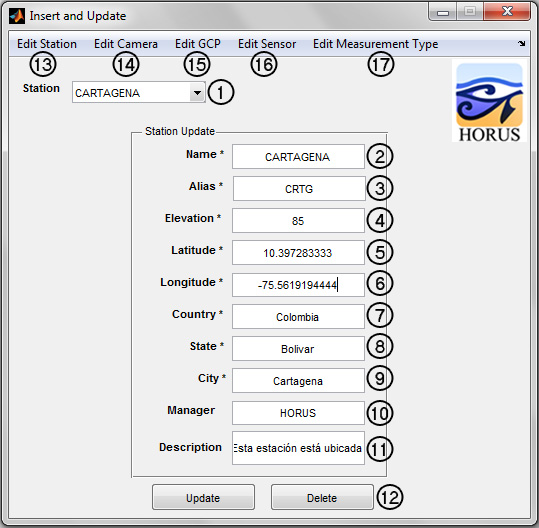
\includegraphics[width=0.6\textwidth]{img/station2}
  \caption{Interfaz para actualizar estaci�n}
  \label{fig:station2}
\end{figure}

Las componentes numeradas en la figura se explican a continuaci�n (los
campos que tienen * son obligatorios):

\begin{enumerate}
\item En esta lista se debe seleccionar la estaci�n que se desea
  actualizar o insertar una nueva estaci�n en caso de escoger la
  opci�n ``\textit{New station}''.
\item Nombre de la estaci�n, �ste debe ser diferente al nombre de las
  dem�s estaciones y no es posible actualizarlo.
\item Alias de la estaci�n, generalmente, una abreviatura del nombre
  de la estaci�n. Debe ser de m�ximo 5 caracteres. �ste debe ser
  diferente al alias de las dem�s estaciones y no es posible
  actualizarlo.
\item Elevaci�n de la estaci�n, �ste es un valor num�rico posiblemente
  con cifras decimales despu�s del (.).
\item Latitud de la estaci�n, �ste es un valor num�rico posiblemente
  con cifras decimales despu�s del (.).
\item Longitud de la estaci�n, �ste es un valor num�rico posiblemente
  con cifras decimales despu�s del (.).
\item Pa�s en donde se encuentra la estaci�n.
\item Estado del pa�s donde se encuentra la estaci�n.
\item Ciudad del estado donde se encuentra la estaci�n.
\item Nombre del responsable de la estaci�n (opcional).
\item Descripci�n general de la estaci�n (opcional).
\item Botones para insertar/actualizar y eliminar el �tem
  seleccionado. El primer bot�n se habilita cuando se ha ingresado la
  informaci�n correctamente, y se comprueba que no haya campos vac�os
  que sean obligatorios y los campos (3), (4) y (5) sean num�ricos. El
  segundo bot�n se habilita cuando se selecciona la estaci�n en el
  campo (1). Al terminar, se mostrar� una ventana indicando el �xito o
  el fracaso de la operaci�n.
\item Men� para insertar, actualizar o eliminar una estaci�n.
\item Men� para insertar, actualizar o eliminar una c�mara.
\item Men� para insertar, actualizar o eliminar un GCP.
\item Men� para insertar, actualizar o eliminar un sensor.
\item Men� para insertar, actualizar o eliminar un tipo de
  medici�n.
\end{enumerate}



En la figura~\ref{fig:station3} se muestra un diagrama de flujo que
explica los procesos de la interfaz donde para cada proceso se nombra
la funci�n que utiliza.

\begin{figure}[htbp!]
  \centering
  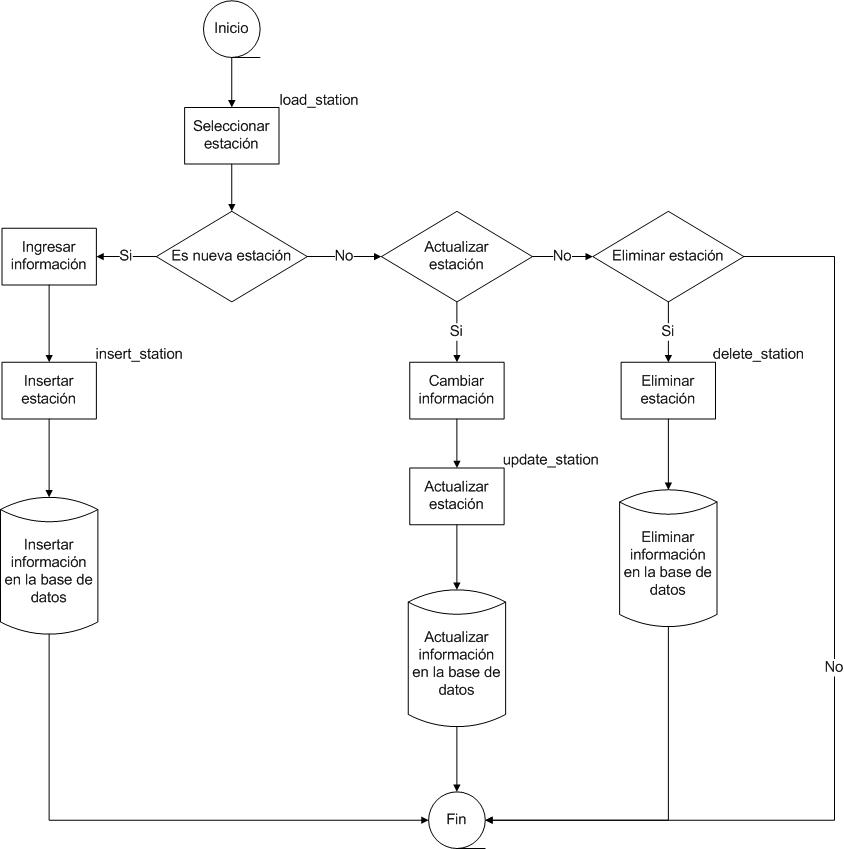
\includegraphics[width=\textwidth]{img/station3}
  \caption{Diagrama de flujo interfaz DB Editor - Estaci�n}
  \label{fig:station3}
\end{figure}


\subsection{C�mara}

En la figura~\ref{fig:camera} se muestra la opci�n de insertar una
c�mara en la base de datos y en la figura~\ref{fig:camera2} la
opci�n de actualizar o eliminar.

\begin{figure}[htbp!]
  \centering
  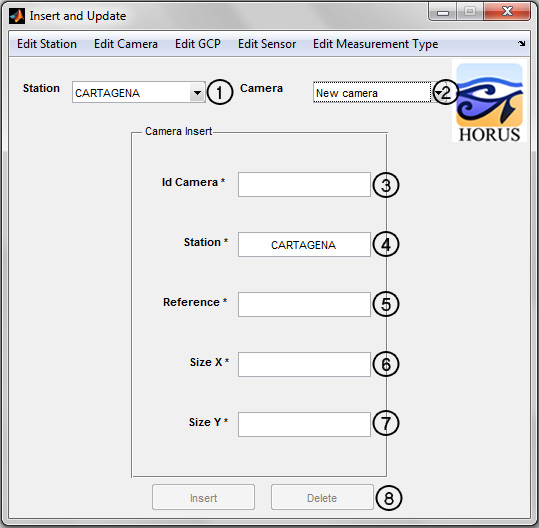
\includegraphics[width=0.6\textwidth]{img/camera}
  \caption{Interfaz para insertar una nueva c�mara}
  \label{fig:camera}
\end{figure}

\begin{figure}[htbp!]
  \centering
  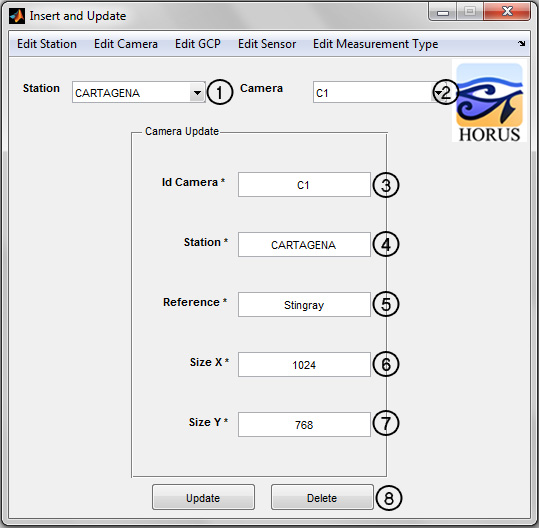
\includegraphics[width=0.6\textwidth]{img/camera2}
  \caption{Interfaz para actualizar una c�mara}
  \label{fig:camera2}
\end{figure}

Las componentes numeradas en la figura se explican a continuaci�n (los
campos que tienen * son obligatorios):

\begin{enumerate}

\item En esta lista se debe seleccionar la estaci�n en la cual se
  encuentra la c�mara a actualizar o en donde se desea insertar una
  nueva c�mara.
\item En esta lista se debe seleccionar la c�mara que se desea
  actualizar o insertar una nueva c�mara en caso de escoger la opci�n
  ``\textit{New camera}''.
\item ID para la c�mara, por lo general es 'C' seguido de un
  n�mero. �ste debe ser �nico para cada estaci�n y no es posible
  actualizarlo.
\item En este campo se visualiza la estaci�n asociada a la
  c�mara. Este campo no es posible actualizarlo.
\item Referencia de la c�mara.
\item Ancho de la imagen capturada por la c�mara. Este valor debe ser
  num�rico y entero.
\item Alto de la imagen capturada por la c�mara. Este valor debe ser
  num�rico y entero.
\item Botones para insertar/actualizar y el otro para eliminar una
  c�mara. El primer bot�n se habilita cuando se ha ingresado la
  informaci�n correctamente, y se comprueba que no haya campos vac�os
  y que los campos (6) y (7) sean num�ricos. El segundo bot�n se
  habilita cuando se selecciona la estaci�n en la lista (1) y la
  c�mara en la lista (2). Al terminar, se mostrar� una ventana
  indicando el �xito o el fracaso de la operaci�n.
\end{enumerate}

En la figura~\ref{fig:camera3} se muestra un diagrama de flujo que
explica los procesos de la interfaz donde para cada proceso se nombra
la funci�n que utiliza.

\begin{figure}[htbp!]
  \centering
  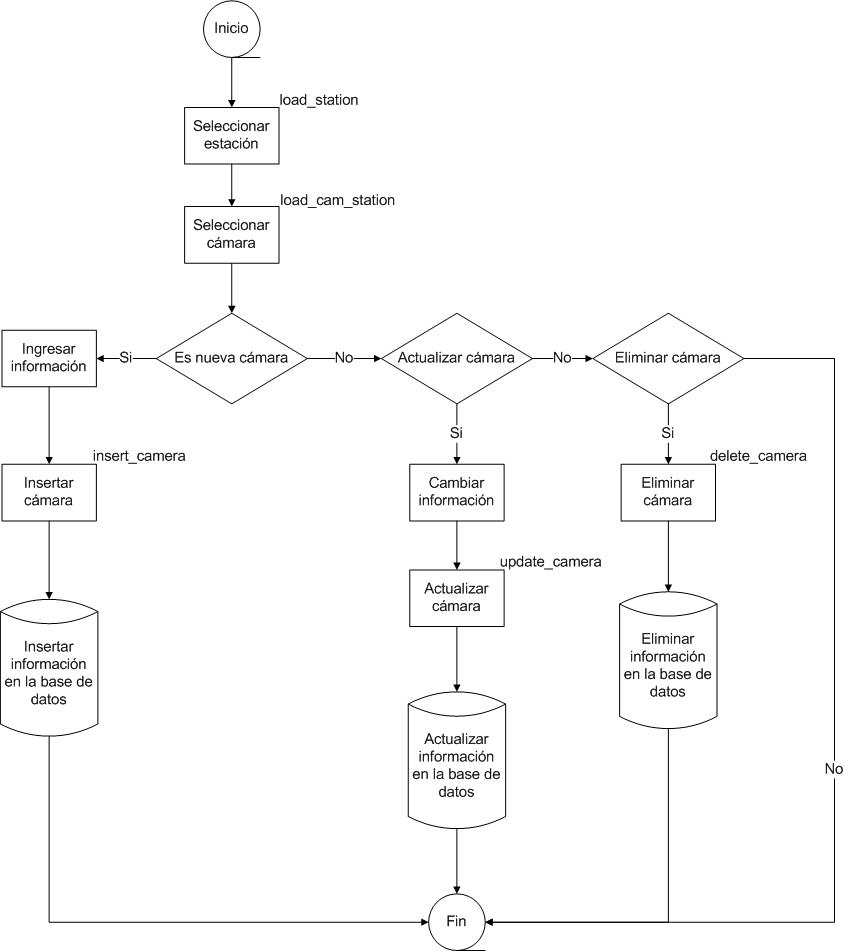
\includegraphics[width=\textwidth]{img/camera3}
  \caption{Diagrama de flujo interfaz DB Editor - C�mara}
  \label{fig:camera3}
\end{figure}

\subsection{GCP}

En la figura~\ref{fig:gcp} se muestra la opci�n de insertar un punto
de control (GCP) en la base de datos y en la figura~\ref{fig:gcp2} la
opci�n de actualizar o eliminar.

\begin{figure}[htbp!]
  \centering
  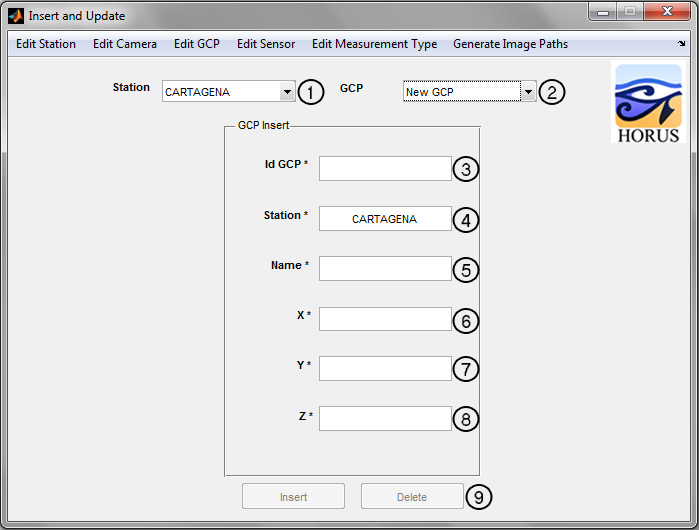
\includegraphics[width=0.6\textwidth]{img/gcp}
  \caption{Interfaz para insertar un nuevo GCP}
  \label{fig:gcp}
\end{figure}

\begin{figure}[htbp!]
  \centering
  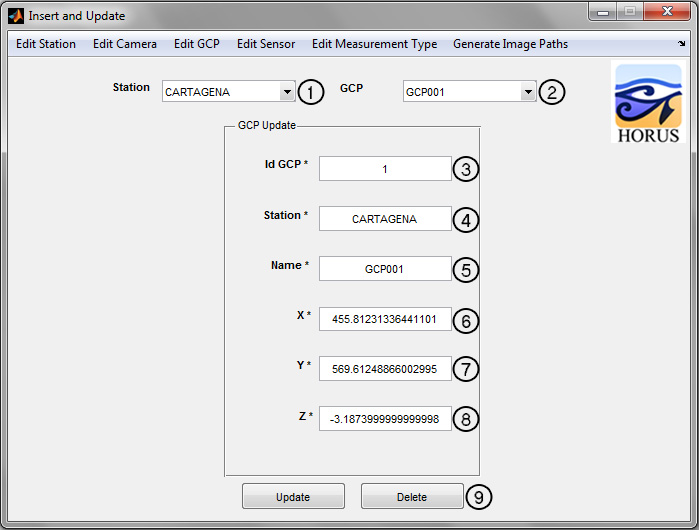
\includegraphics[width=0.6\textwidth]{img/gcp2}
  \caption{Interfaz para actualizar un GCP}
  \label{fig:gcp2}
\end{figure}

Las componentes numeradas en la figura se explican a continuaci�n (los
campos que tienen * son obligatorios):

\begin{enumerate}
\item En esta lista se debe seleccionar la estaci�n en la cual se
  encuentra el GCP a actualizar o insertar.
\item En esta lista se debe seleccionar el GCP que se desea actualizar
  o insertar un nuevo GCP en caso de escoger la opci�n ``\textit{New
    GCP}''. Hay otra opci�n en esta lista para importar GCPs desde un
  archivo de Excel externo. Al seleccionar esta opci�n, se abre una
  nueva ventana para seleccionar un archivo de Excel que debe contener
  los datos de los GCPs que se desean importar a la base de datos. El
  archivo de Excel debe tener la estructura mostrada en la
  figura~\ref{fig:gcp_excel}. Las columnas contienen en orden, los IDs
  de los GCPs los cuales deben ser num�ricos y �nicos para cada
  estaci�n, los nombres de los GCPs los cuales deben ser �nicos para
  cada estaci�n, los valores de la coordenada $X$, $Y$ y $Z$ del GCP
  en el sistema coordenado correspondiente, estas tres �ltimas
  columnas deben ser num�ricas. El archivo de Excel solo debe tener
  una hoja de calculo, todas las dem�s deben ser eliminadas, tambi�n
  el separador decimal del archivo debe ser un punto (.) en caso de
  que sea una coma (,) se debe proceder a cambiarlo, esto con el fin
  de garantizar un buen funcionamiento del sistema.

\begin{figure}[htbp!]
  \centering
  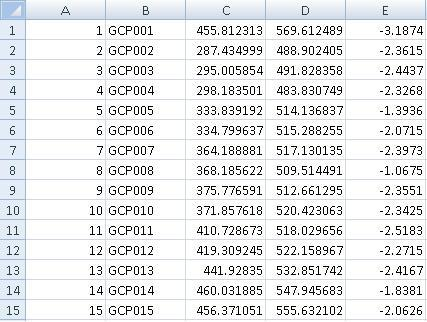
\includegraphics[width=0.6\textwidth]{img/gcp_excel}
  \caption{Estructura de excel para importar GCPs}
  \label{fig:gcp_excel}
\end{figure}

Este archivo no debe tener ning�n encabezado, la primera fila debe
contener los datos del primer GCP a insertar en la base de
datos. Despu�s de seleccionar el archivo se debe dar clic en el bot�n
insertar. Al terminar el proceso saldr� un mensaje indicando la
cantidad de GCPs insertados exitosamente. Se debe tener en cuenta que
los GCPs importados no reemplazar�n los existentes haciendo las veces
de actualizaci�n, si se desean actualizar se deber�n eliminar todos y
luego importarlos o hacerlo uno a la vez.
 
En las opciones, tambi�n se puede seleccionar o eliminar todos los
GCPs (incluyendo las marcaciones del usuario) en la estaci�n que se
seleccion� anteriormente.  Despu�s de seleccionar esta opci�n se debe
dar clic en el bot�n ``\textit{Delete}'', al terminar el proceso
saldr� un mensaje indicando el �xito o el fracaso de la operaci�n.
\item ID para el GCP, �ste debe ser �nico para cada estaci�n, ser
  num�rico y entero. Este campo no es posible actualizarlo.
\item Estaci�n asociada al GCP. Este campo no es posible actualizarlo.
\item Nombre del GCP, por lo general es GCP y tres d�gitos (e.g.\
  GCP001). Este campo debe ser �nico para cada estaci�n.
\item Valor de la coordenada $x$ del GCP en el sistema coordenado
  correspondiente. �ste es un valor num�rico posiblemente con cifras
  decimales despu�s del (.).
\item Valor de la coordenada $y$ del GCP en el sistema coordenado
  correspondiente. �ste es un valor num�rico posiblemente con cifras
  decimales despu�s del (.).
\item Valor de la coordenada $z$ del GCP en el sistema coordenado
  correspondiente. �ste es un valor num�rico posiblemente con cifras
  decimales despu�s del (.).
\item Botones para insertar/actualizar y eliminar un GCP. El primer
  bot�n se habilita cuando se ha ingresado la informaci�n
  correctamente, y se comprueba que no haya campos vac�os y los campos
  (6), (7) y (8) sean num�ricos. El segundo bot�n se habilita cuando
  se selecciona la estaci�n en la lista (1) y el GCP en la lista
  (2). Al terminar se mostrar� una ventana indicando el �xito o el
  fracaso de la operaci�n.
\end{enumerate}



En la figura~\ref{fig:gcp3} se muestra un diagrama de flujo que
explica los procesos de la interfaz donde para cada proceso se nombra
la funci�n que utiliza.

\begin{figure}[htbp!]
  \centering
  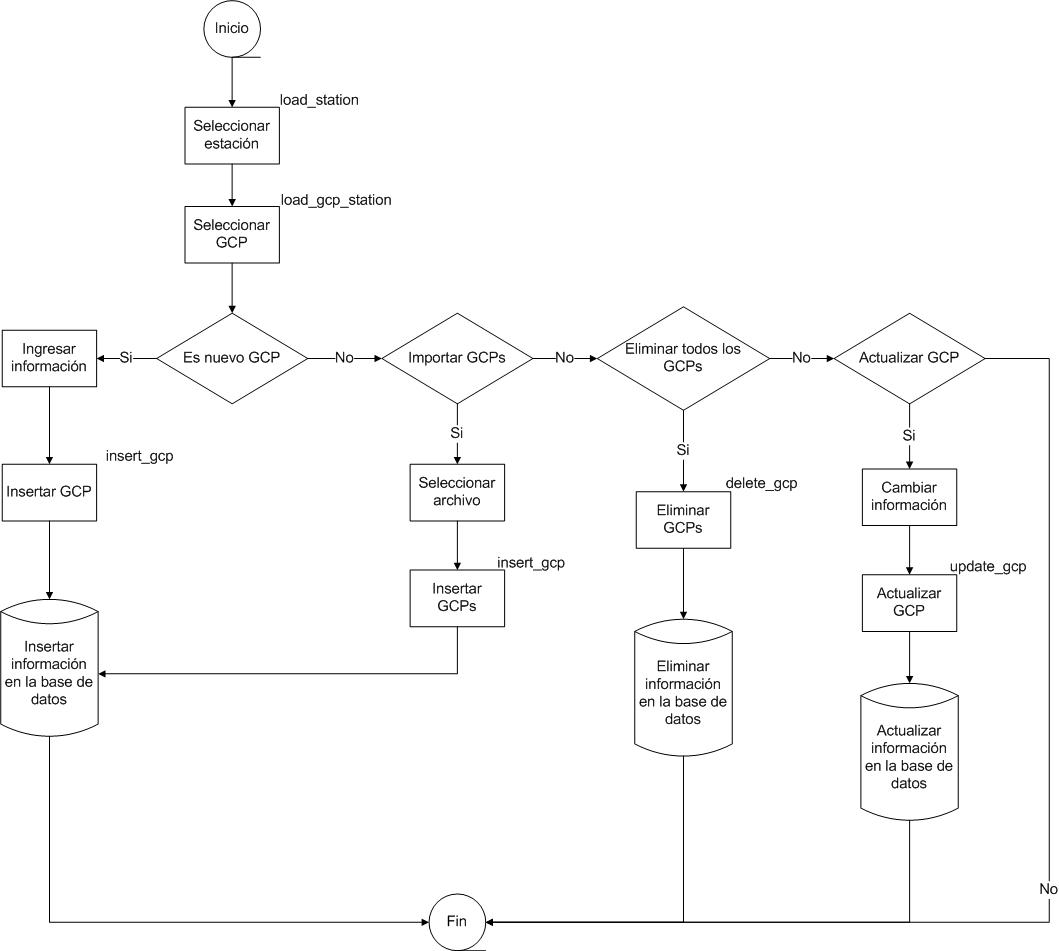
\includegraphics[width=\textwidth]{img/gcp3}
  \caption{Diagrama de flujo interfaz DB Editor - GCP}
  \label{fig:gcp3}
\end{figure}

\subsection{Sensor}


Los sensores son los equipos utilizados para hacer mediciones, por
ejemplo, una boya puede medir altura de ola, per�odo de ola, entre
otros. En la figura~\ref{fig:sensor} se muestra la opci�n de insertar
un sensor en la base de datos y en la figura~\ref{fig:sensor2} la
opci�n de actualizar o eliminar.

\begin{figure}[htbp!]
  \centering
  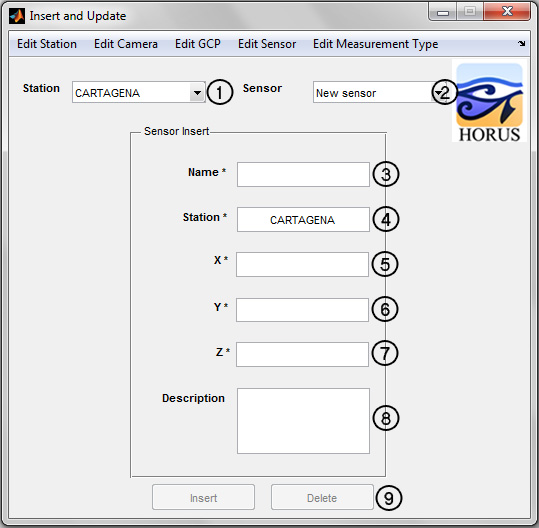
\includegraphics[width=0.6\textwidth]{img/sensor}
  \caption{Interfaz para insertar un nuevo sensor}
  \label{fig:sensor}
\end{figure}

\begin{figure}[htbp!]
  \centering
  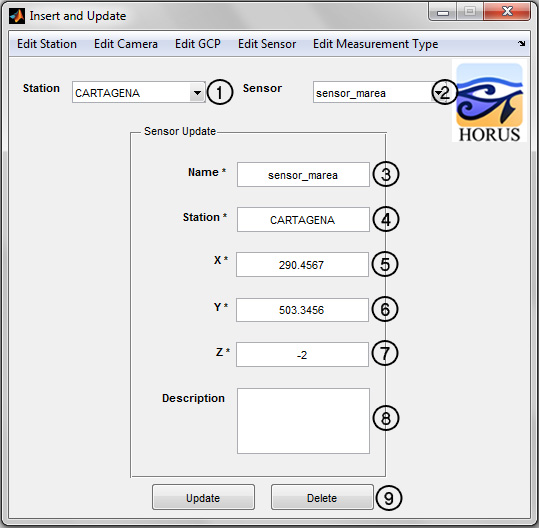
\includegraphics[width=0.6\textwidth]{img/sensor2}
  \caption{Interfaz para actualizar un sensor}
  \label{fig:sensor2}
\end{figure}


Las componentes numeradas en la figura se explican a continuaci�n (los
campos que tienen * son obligatorios):

\begin{enumerate}
\item En esta lista se debe seleccionar la estaci�n en la cual se
  encuentra el sensor a actualizar o en donde se desea insertar el
  sensor.
\item En esta lista se debe seleccionar el sensor que se desea
  actualizar o insertar un nuevo sensor en caso de escoger la opci�n
  ``\textit{New sensor}''.
\item Nombre para el sensor el cual debe ser �nico para cada
  estaci�n. Este campo no es posible actualizarlo.
\item Estaci�n asociada al sensor. Este campo no es posible
  actualizarlo.
\item Valor de la coordenada $x$ del sensor en el sistema coordenado
  correspondiente. �ste es un valor num�rico posiblemente con cifras
  decimales despu�s del (.).
\item Valor de la coordenada $y$ del sensor en el sistema coordenado
  correspondiente. �ste es un valor num�rico posiblemente con cifras
  decimales despu�s del (.).
\item Valor de la coordenada $z$ del sensor en el sistema coordenado
  correspondiente. �ste es un valor num�rico posiblemente con cifras
  decimales despu�s del (.).
\item Descripci�n verbal del sensor.
\item Botones para insertar/actualizar y eliminar un sensor. El primer
  bot�n se habilita cuando se ha ingresado la informaci�n
  correctamente, se comprueba que s�lo el campo de descripci�n pueda
  estar vac�o y los campos (5), (6) y (7) sean num�ricos. El segundo
  bot�n se habilita cuando se selecciona la estaci�n en la lista (1) y
  el sensor en la lista (2). Al terminar, se mostrar� una ventana
  indicando el �xito o el fracaso de la operaci�n.
\end{enumerate}

En la figura~\ref{fig:sensor3} se muestra un diagrama de flujo que
explica los procesos de la interfaz donde para cada proceso se nombra
la funci�n que utiliza.

\begin{figure}[htbp!]
  \centering
  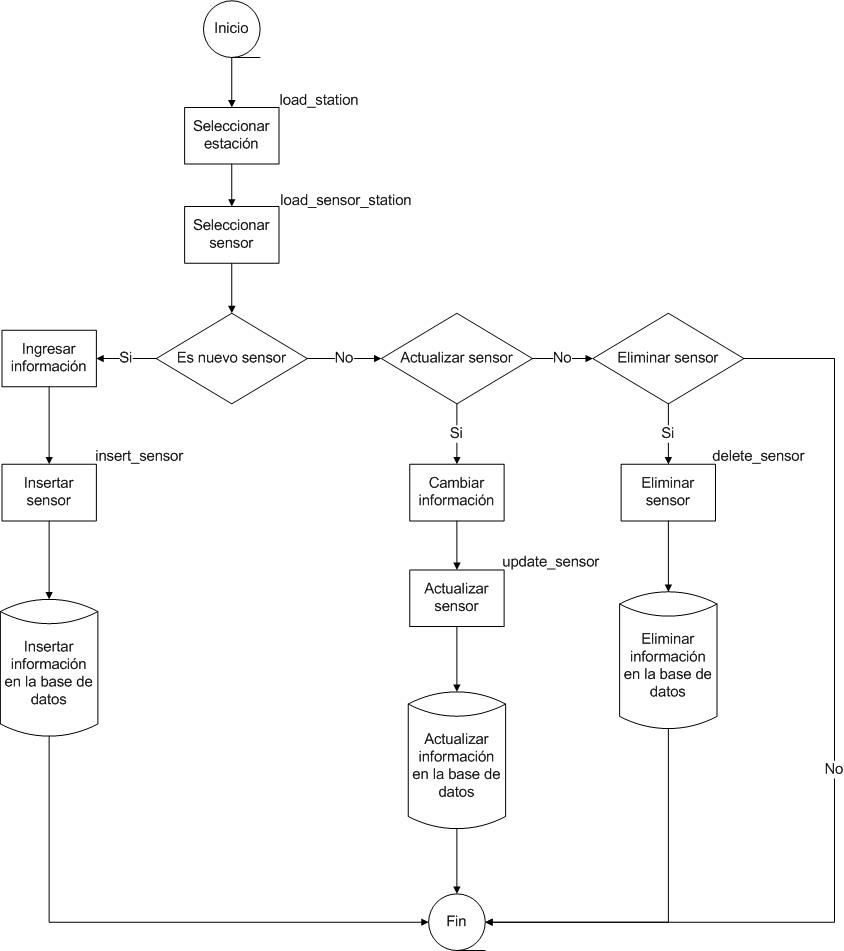
\includegraphics[width=\textwidth]{img/sensor3}
  \caption{Diagrama de flujo interfaz DB Editor - Sensor}
  \label{fig:sensor3}
\end{figure}

\subsection{Tipo de Medici�n}


Los tipos de medici�n son los par�metros que pueden ser medidos por
un sensor, por ejemplo, marea, altura significante de ola, per�odo
pico del oleaje, entre otros.  Un tipo de medici�n siempre depende
de un sensor, si no se tiene la informaci�n exacta del sensor se
podr�n crear sensores artificiales. Pueden haber varios tipos de
mediciones asociadas a un sensor.

En la figura~\ref{fig:measurementtype} se muestra la opci�n de
insertar un tipo de medici�n en la base de datos y en la
figura~\ref{fig:measurementtype2} la opci�n de actualizar o eliminar.

\begin{figure}[htbp!]
  \centering
  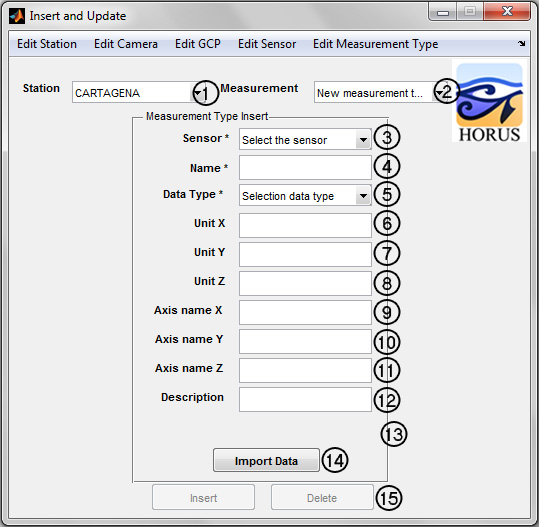
\includegraphics[width=0.6\textwidth]{img/measurementtype}
  \caption{Interfaz para insertar un nuevo tipo de medici�n}
  \label{fig:measurementtype}
\end{figure}

\begin{figure}[htbp!]
  \centering
  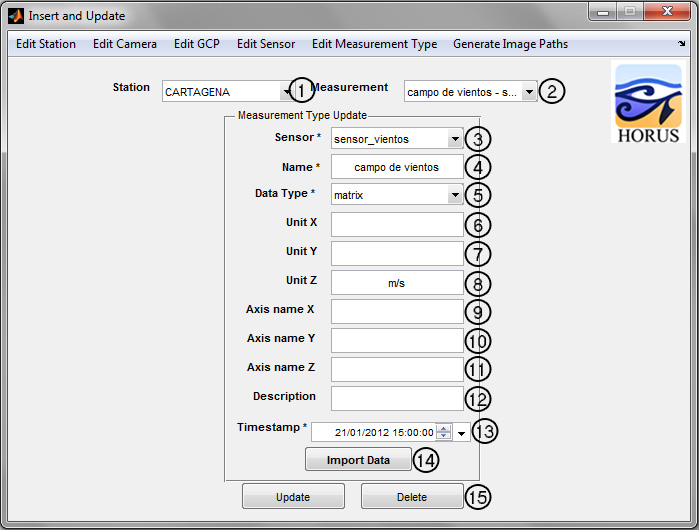
\includegraphics[width=0.6\textwidth]{img/measurementtype2}
  \caption{Interfaz para actualizar un tipo de medici�n}
  \label{fig:measurementtype2}
\end{figure}

Las componentes numeradas en la figura se explican a continuaci�n (los
campos que tienen * son obligatorios):

\begin{enumerate}
\item En esta lista se debe seleccionar la estaci�n en la cual se
  encuentra el tipo de medici�n a actualizar o en donde se desea
  insertar el tipo de medici�n.
\item En esta lista se debe seleccionar el tipo de medici�n que se
  desea actualizar o insertar un nuevo tipo de medici�n en caso de
  escoger la opci�n ``\textit{New measurement type}''.
\item En esta lista se debe seleccionar el sensor con el cual se
  hicieron las mediciones.
\item Nombre del par�metro medido, el cual debe ser �nico para cada
  estaci�n y de preferencia que sea una abreviatura. Este campo no es
  posible actualizarlo.
\item Lista con los tipos de dato que puede ser ``time series'' si los
  datos son de una serie de tiempo, o ``matrix'' si los datos son en
  tres dimensiones.
\item Abreviatura de la unidad de medida del eje horizontal ($x$).  Si
  es una serie de tiempo ser�a la unidad de tiempo (horas, minutos).
\item Abreviatura de la unidad de medida del eje vertical ($y$).
\item Abreviatura de la unidad de medida del eje $z$.  Si es una serie
  de tiempo este campo se desactiva.
\item Etiqueta del eje $x$ en la gr�fica. Este campo no es necesario
  si es una serie de tiempo.
\item Etiqueta del eje $y$ en la gr�fica. Este campo no es necesario
  si es una serie de tiempo.
\item T�tulo de la gr�fica si se trata de un tipo de dato matriz, en
  caso contrario se desactiva.
\item Descripci�n del tipo de medici�n.
\item En caso de ser datos de tipo matriz se mostrar� un calendario en
  donde se escoger� la fecha de la medici�n. �ste puede tomar
  cualquier fecha menor al instante en que se est� haciendo la
  inserci�n.
\item Bot�n para agregar los datos de la medici�n a la base de
  datos, el cual es obligatorio s�lo si se desea agregar
  informaci�n. Dando clic en este bot�n se abrir� una ventana en la
  cual se escoger� el archivo que tiene los datos de la
  medici�n. Este archivo puede tener format MAT o Excel, y no debe
  tener ning�n encabezado.  La estructura que debe tener el archivo es
  la siguiente:

  Si el tipo de dato es serie de tiempo, en la primera columna debe
  estar la fecha de la medici�n en el formato que utiliza la
  funci�n \texttt{datenum} de MATLAB. En la segunda columna debe estar
  el valor de la medici�n para esa fecha.  En la
  figura~\ref{fig:measurementtype_series} se muestra la estructura
  necesaria.

\begin{figure}[htbp!]
  \centering
  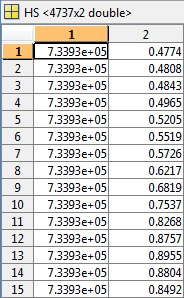
\includegraphics[width=0.3\textwidth]{img/measurementtype_series}
  \caption{Estructura de MATLAB si el tipo de medici�n es serie}
  \label{fig:measurementtype_series}
\end{figure}

Si el tipo de dato es matriz en la primera columna se debe poner el
valor de $x$ en la segunda columna el valor de $y$ y en la tercera el
valor de $z$.  En la figura~\ref{fig:measurementtype_matrix} se
muestra la estructura necesaria.

\begin{figure}[htbp!]
  \centering
  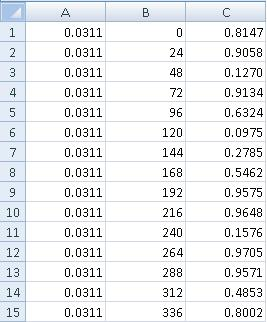
\includegraphics[width=0.4\textwidth]{img/measurementtype_matrix}
  \caption{Estructura de Excel si el tipo de medici�n es matriz}
  \label{fig:measurementtype_matrix}
\end{figure}

Si el archivo tiene formato MAT, �ste s�lo podr� contener una matriz
que tenga los datos, si el archivo es de Excel s�lo debe tener una
hoja de c�lculo, todas las dem�s deben ser eliminadas, tambi�n el
separador decimal del archivo debe ser un punto (.) en caso de que sea
una coma (,) se debe proceder a cambiarlo esto con el fin de
garantizar un buen funcionamiento del sistema.

\item Botones para insertar/actualizar y eliminar un tipo de
  medici�n. El primer bot�n se habilita cuando se ha ingresado la
  informaci�n correctamente, y se comprueba que los campos con * no
  est�n vacios.  El segundo bot�n se habilita cuando se selecciona la
  estaci�n en la lista (1) y el tipo de medici�n en la lista
  (2). Al terminar se mostrar� una ventana indicando el �xito o el
  fracaso de la operaci�n.
\end{enumerate}

Si se ha insertado un tipo de medici�n y luego se quiere agregar
m�s datos a �ste se puede hacer seleccion�ndolo en el campo (2) y luego
seleccionando el archivo por medio del campo (11), y finalmente dando
clic en el bot�n ``\textit{Update}''.

En la figura~\ref{fig:measurementtype3} se muestra un diagrama de
flujo que explica los procesos de la interfaz donde para cada proceso se nombra
la funci�n que utiliza.

\begin{landscape}
  \begin{figure}[htbp!]
    \centering
    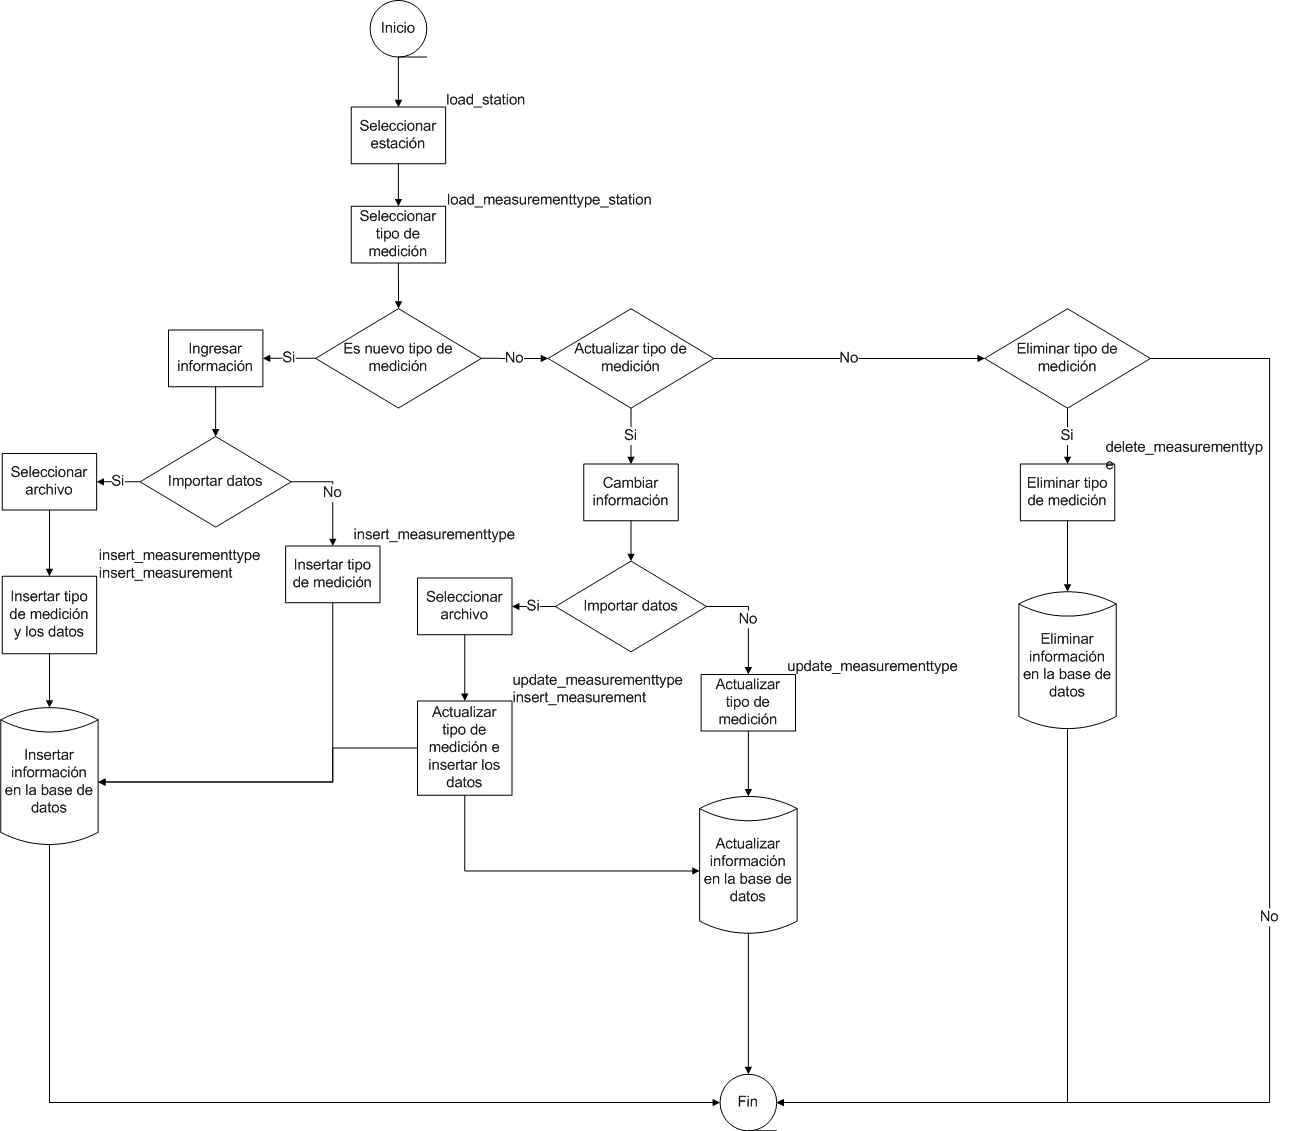
\includegraphics[width=\textwidth]{img/measurementtype3}
    \caption{Diagrama de flujo interfaz DB Editor - Tipo de
        Medici�n}
    \label{fig:measurementtype3}
  \end{figure}
\end{landscape}

\section{Configure cameras}

Luego de configurar las estaciones y las c�maras para cada estaci�n en
la base de datos, es necesario configurar f�sicamente las c�maras para
la captura. En esta secci�n se describe la interfaz utilizada para
llevar a cabo esta tarea, configurar las c�maras conectadas al
computador de captura con los par�metros de captura requeridos. Para
utilizar esta interfaz es necesario disponer del toolbox de
Adquisici�n de Im�genes de MATLAB.

Para configurar las c�maras se debe tener instalado el adaptador
correspondiente en el caso de c�maras \textit{Firewire} o c�maras
web. Si se trata de una c�mara web, por lo general, el sistema
operativo reconoce el controlador, sino, hay que instalarlo
manualmente usando el instalador que provee la marca de la c�mara. Por
ejemplo, si se trata de c�maras \textit{Firewire} AVT (\textit{Allied
  Vision Technologies}) se debe instalar el software
\textit{FirePackage} disponible en la p�gina web
\url{http://www.alliedvisiontec.com/emea/products/software/windows/avt-firepackage.html}.
Para otro tipo de c�maras \textit{Firewire} se debe instalar el
controlador universal CMU disponible en
\url{http://www.cs.cmu.edu/~iwan/1394/}.

Luego de instalar el controlador en el computador, para utilizar las
c�maras en MATLAB es necesario registrar el adaptador correspondiente
con el comando \texttt{imaqregister}. MATLAB dispone de un adaptador
por defecto para las c�maras web; en el sistema operativo Windows,
este adaptador es \texttt{winvideo}; en Linux, es \texttt{linuxvideo}
(\emph{Nota}: Otro adaptador com�n que viene inclu�do en MATLAB es
\texttt{coreco}, para c�maras \textit{DALSA--CORECO}). Si �ste es el
caso, no es necesario registrar un adaptador, pero para otro tipo de
c�maras como las \textit{Firewire}, s� es necesario registrarlo (si
est� soportado por la marca correspondiente). Por ejemplo, si el
adaptador es \texttt{avtmatlabadaptor.dll} (el correspondiente a las
c�maras \textit{Firewire} de la marca AVT) y se encuentra en el
directorio \texttt{C:}, el comando para registrarlo en MATLAB ser�a:
\\
\verb!> imaqregister('C:\avtmatlabadaptor.dll')!.

\verb!> imaqreset!

En la figura~\ref{fig:confcam} se muestra la interfaz de configuraci�n
de c�maras.

\begin{figure}[htbp!]
  \centering
  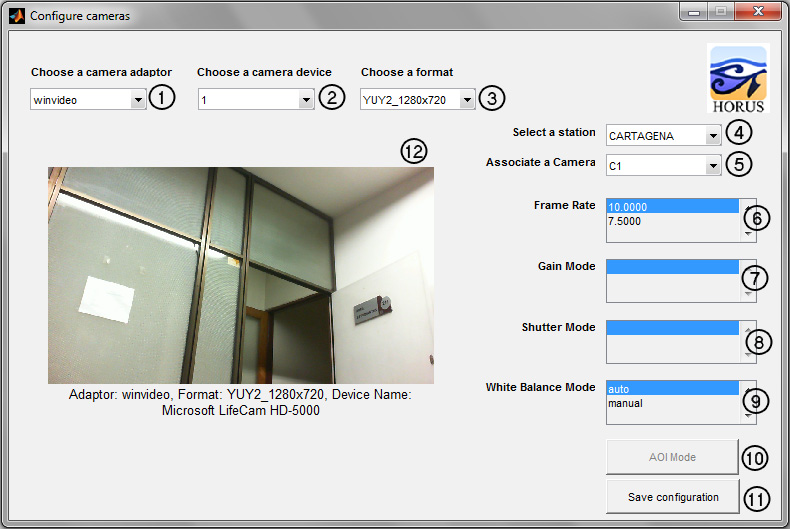
\includegraphics[width=\textwidth]{img/confcam}
  \caption{Interfaz de Configuraci�n de c�maras}
  \label{fig:confcam}
\end{figure}

El comando para ejecutar esta interfaz es:
\texttt{gui\_configure\_cameras}.

Las componentes numeradas en la figura se explican a continuaci�n:

\begin{enumerate}
\item Lista donde se puede escoger el adaptador.
\item Lista para escoger el dispositivo conectado al
  computador de captura.
\item Lista para escoger el formato del dispositivo. Se
  compone de dos partes, el formato de p�xeles (e.g.\@ RGB, YUV) y el
  tama�o de la imagen.
\item Lista para seleccionar la estaci�n de captura,
  previamente almacenada y configurada en la base de datos.
\item Lista para asociar una c�mara previamente
  configurada en la base de datos, con el dispositivo f�sico
  seleccionado actualmente.
\item Lista de \textit{framerates} disponibles para el dispositivo.
\item Modo de ganancia del dispositivo.
\item Modo de disparo del dispositivo.
\item Modo de balance de blancos del dispositivo.
\item Si la c�mara es AVT \textit{Firewire}, se puede
  seleccionar un �rea de inter�s (AOI) la cual es la regi�n de la
  imagen que ser� utilizada para calcular los valores de la Ganancia,
  Disparo y Balance de blancos en caso de ser escogidos en la
  configuraci�n de la c�mara.
\item Bot�n para guardar la configuraci�n de la c�mara. Esta
  configuraci�n se guarda en un archivo XML llamado
  \texttt{capture\_info.xml}.
\item Previsualizaci�n de la imagen de la c�mara.
\end{enumerate}

En la figura~\ref{fig:flow_confcam} se muestra el diagrama de flujo
para la configuraci�n de las c�maras, donde para cada proceso se
nombra la funci�n que utiliza.

\begin{figure}[htbp!]
  \centering
  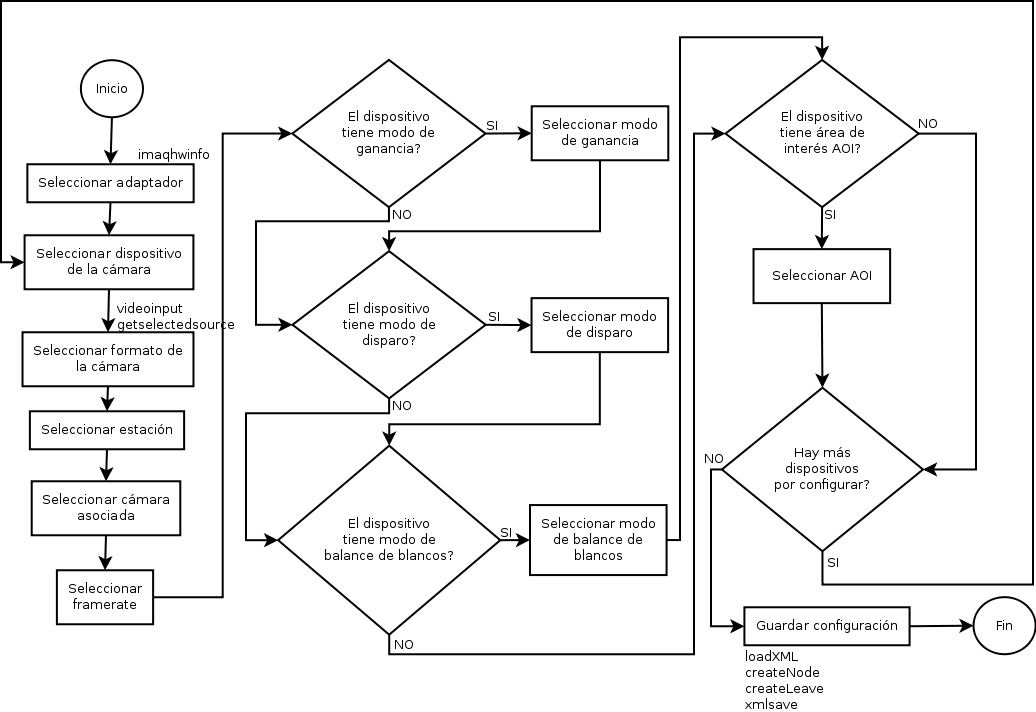
\includegraphics[width=\textwidth]{img/flow_confcam}
  \caption{Diagrama de flujo para el proceso de configuraci�n de las
    c�maras}
  \label{fig:flow_confcam}
\end{figure}


\section{Capture configuration}

En la secci�n anterior, se mostr� la interfaz para configurar las
c�maras de captura despu�s de haber sido asociadas con las c�maras de
la base de datos. En esta secci�n, se muestra la interfaz para
configurar la captura como tal, entre las cosas que se configuran se
encuentran las horas del d�a en que se capturan im�genes y
\textit{stacks}, as� como la informaci�n para el env�o de los
datos. La configuraci�n se guarda en el archivo XML
\texttt{capture\_info.xml} que se utiliza por el programa autom�tico
de captura.

En la figura~\ref{fig:captureconf} se muestra la interfaz de
configuraci�n de captura.

\begin{figure}[htbp!]
  \centering
  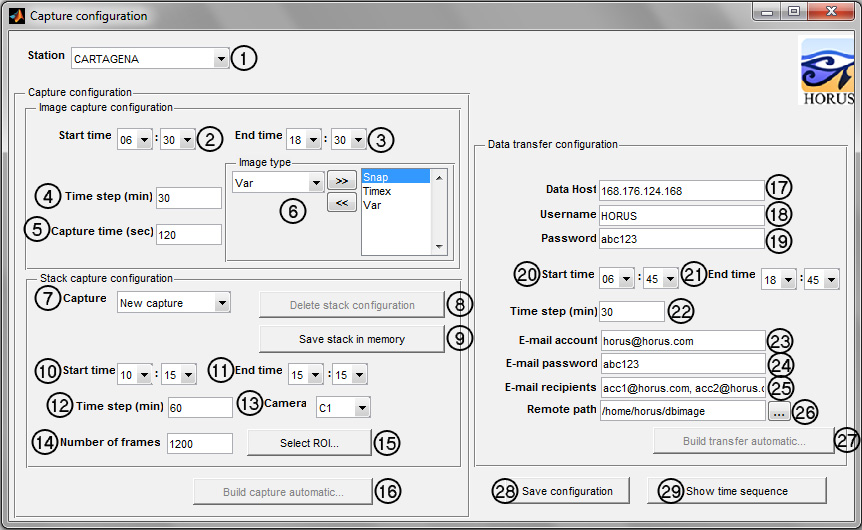
\includegraphics[width=\textwidth]{img/captureconf}
  \caption{Interfaz de Configuraci�n de capturas}
  \label{fig:captureconf}
\end{figure}

El comando para ejecutar esta interfaz es:
\texttt{gui\_configure\_capture}.

Las componentes numeradas en la figura se explican a continuaci�n:

\begin{enumerate}
\item Lista desplegable para seleccionar la estaci�n.
\item Tiempo inicial de la captura de im�genes.
\item Tiempo final de la captura de im�genes.
\item Tama�o de paso entre captura y captura, en minutos.
\item Tiempo de captura, en segundos.
\item Tipos de im�genes que se desean capturar.
\item Lista desplegable donde se puede seleccionar una configuraci�n
  de captura de \textit{stacks} para actualizaci�n o la opci�n de
  crear una nueva configuraci�n.
\item Bot�n para eliminar la configuraci�n de \textit{stacks}
  seleccionada (s�lo se habilita si hay una configuraci�n
  seleccionada).
\item Bot�n para guardar en memoria la configuraci�n de
  \textit{stacks} actual. Esta configuraci�n solamente se guarda en el
  archivo \texttt{capture\_info.xml} al presionar el bot�n
  \textit{Save configuration}.
\item Tiempo inicial de la captura de \textit{stacks}.
\item Tiempo final de la captura de \textit{stacks}.
\item Tama�o de paso entre captura y captura, en minutos.
\item Lista de las c�maras guardadas en la base de datos, se debe
  seleccionar una para asociarla a la captura.
\item N�mero de frames del v�deo. El \textit{framerate} de la captura
  es el mismo que se eligi� al configurar la c�mara.
\item Bot�n para escoger una regi�n de inter�s para la captura. La
  regi�n de inter�s se define como el conjunto de coordenadas $(u, v)$
  de un pol�gono cerrado dentro de la imagen, en sentido horario o
  antihorario. Para seleccionar un ROI, se debe haber configurado la
  c�mara seleccionada de antemano; al presionar este bot�n, la c�mara
  captura una imagen y la muestra para seleccionar los puntos
  correspondientes a los v�rtices del pol�gono que conforma el ROI.
\item Bot�n para generar el autom�tico de captura de im�genes y
  \textit{stacks}.
\item La configuraci�n del env�o de datos contiene varios campos. Este
  campo es la direcci�n del servidor SSH al que se env�an las
  im�genes.
\item Nombre de usuario del cliente SSH.
\item Contrase�a del cliente SSH.
\item Tiempo inicial del env�o.
\item Tiempo final del env�o.
\item Tama�o de paso entre env�o y env�o, en minutos.
\item Cuenta de e--mail desde donde se env�an mensajes de error sobre
  el env�o de datos.
\item Contrase�a de la cuenta de e--mail.
\item Lista de e--mails separados por comas que reciben los mensajes
  de error.
\item Ruta remota en el servidor en donde se almacenar�n los datos
  enviados.
\item Bot�n para generar el autom�tico de transferencia.
\item Bot�n para almacenar la configuraci�n en el archivo XML y en la
  base de datos (si todos los campos son v�lidos y no hay solapamiento
  entre tiempos de captura).
\item Bot�n que muestra gr�ficamente los tiempos de captura,
  transferencia y procesamiento previamente configurados.
\end{enumerate}

En la figura~\ref{fig:flow_captureconf} se muestra el diagrama de
flujo para la configuraci�n de capturas, donde para cada proceso se
nombra la funci�n que utiliza.

\begin{figure}[htbp!]
  \centering
  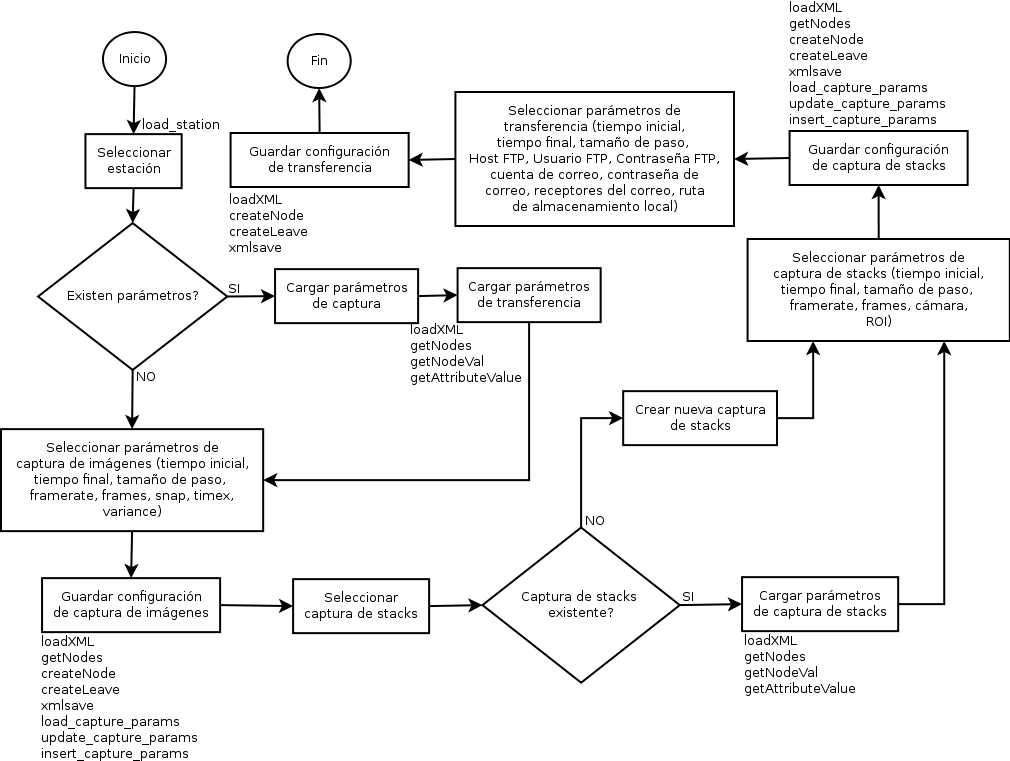
\includegraphics[width=\textwidth]{img/flow_captureconf}
  \caption{Diagrama de flujo del proceso de configuraci�n de captura}
  \label{fig:flow_captureconf}
\end{figure}

Toda esta informaci�n es utilizada por el algoritmo autom�tico que
lleva a cabo la captura. En la figura~\ref{fig:flow_autocapture} se
muestra el diagrama de flujo que describe el proceso de este
autom�tico. El autom�tico se ejecuta como un servicio o demonio, es
decir, se ejecuta infinitamente hasta que ocurre un evento que dispara
una acci�n, en este caso, ese evento son las horas programadas para
realizar la captura.

\begin{landscape}
  \begin{figure}[htbp!]
    \centering
    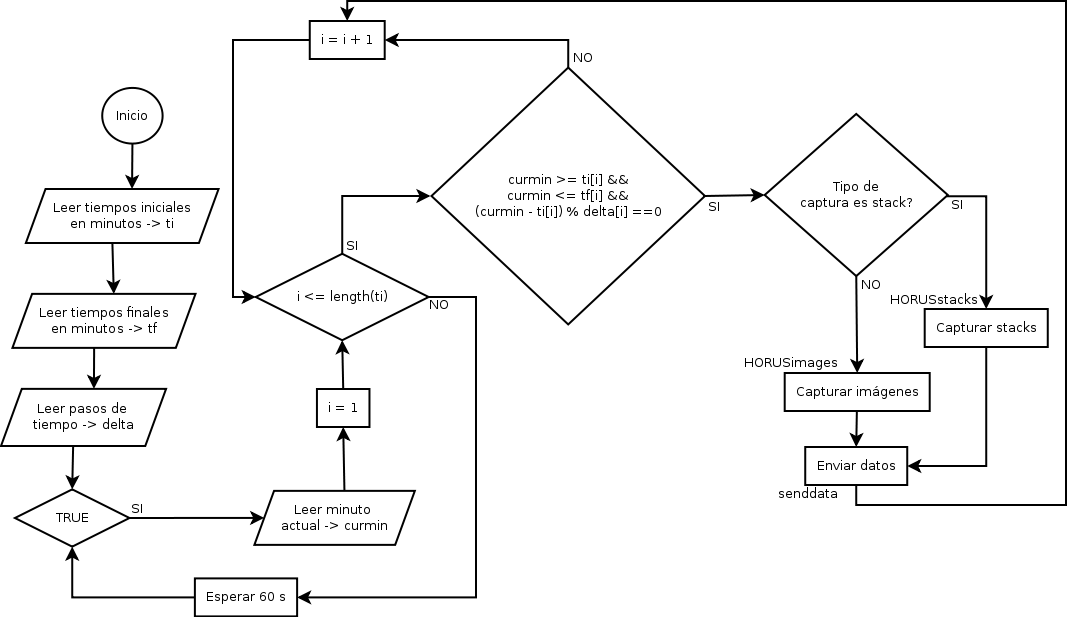
\includegraphics[height=0.8\textwidth]{img/flow_autocapture}
    \caption{Diagrama de flujo del autom�tico de captura}
    \label{fig:flow_autocapture}
  \end{figure}
\end{landscape}

Para utilizar el autom�tico de captura, es necesario compilar las
funciones \verb!auto_capture_images.m! y \verb!auto_transfer.m! del
directorio \texttt{src}, mediante los botones correspondientes en la
interfaz. Sin embargo, si se quieren compilar manualmente, se ejecutan
los siguientes comandos en la l�nea de comandos de MATLAB (suponiendo
que el directorio de HORUS es \verb!C:\horus!):

\begin{flushleft}
  \verb!cd C:\horus!

  \verb!addpath('src')!

  \verb!mcc -m auto_capture_images -a ./data -I ./tmp!

  \verb!mcc -m auto_transfer -a ./data -I ./tmp!

\end{flushleft}

Si la compilaci�n se realiz� mediante la interfaz, se generan los
archivos ejecutables \texttt{run\_auto\_capture\_images.bat} y
\texttt{run\_auto\_transfer.bat}.

Si los archivos se compilaron manualmente, en el sistema operativo
Windows, se generan dos ejecutables \texttt{auto\_capture\_images.exe}
y \texttt{auto\_transfer.exe}, los cuales reciben unos par�metros de
entrada. El autom�tico de captura recibe el nombre de la estaci�n, y
el autom�tico de transferencia recibe el nombre de la estaci�n y la
direcci�n IP del servidor al que se enviar�n los datos. Para
ejecutarlos, se debe crear para cada uno, un archivo BAT que recibe
los par�metros. Un ejemplo de archivo BAT para el autom�tico de
captura podr�a contener el siguiente c�digo
(\texttt{run\_auto\_capture\_images.bat}):

\begin{flushleft}
  \verb!auto_capture_images.exe CARTAGENA!
\end{flushleft}

Para el autom�tico de transferencia (\texttt{run\_auto\_transfer.bat}):

\begin{flushleft}
   \verb!auto_transfer.exe CARTAGENA 168.176.124.165!
\end{flushleft}

\emph{Nota:} Es posible que al compilar el autom�tico de transferencia
aparezca un mensaje de advertencia. Esto es normal y se puede hacer
caso omiso de �l.

\section{Path Editor}

Actualmente, el sistema HORUS trabaja cuatro tipos de im�genes:
oblicuas, rectificadas, oblicuas--fusionadas y
rectificadas--fusionadas, pero se pueden agregar m�s a la base de
datos cuando sea necesario. De cada uno de estos tipos se pueden
generar im�genes miniaturas.

En esta secci�n se describe la interfaz que sirve para configurar las
rutas de almacenamiento en disco de cada uno de estos tipos de
im�genes. En total, son ocho rutas que se deben configurar.

El Toolbox de HORUS cuenta con un archivo XML que contiene las rutas a
las im�genes de cada estaci�n, \texttt{path\_info.xml}. Con esta
interfaz se pueden editar estas rutas. En las
figuras~\ref{fig:edit_path} y~\ref{fig:edit_path2} se muestra la
interfaz.

\begin{figure}[htbp!]
  \centering
  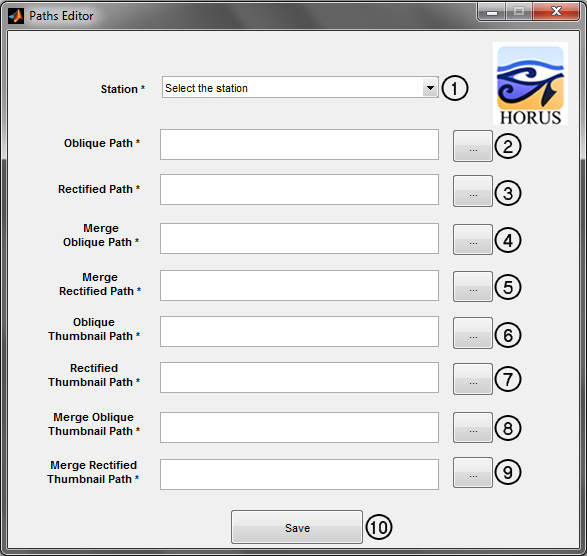
\includegraphics[width=0.6\textwidth]{img/edit_path}
  \caption{Interfaz inicial para editar las rutas}
  \label{fig:edit_path}
\end{figure}



\begin{figure}[htbp!]
  \centering
  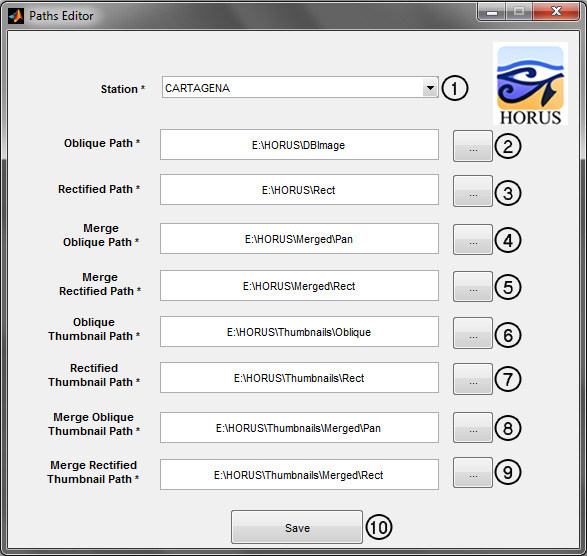
\includegraphics[width=0.6\textwidth]{img/edit_path2}
  \caption{Interfaz para editar las rutas ya con cambios realizados}
  \label{fig:edit_path2}
\end{figure}

El comando para ejecutar esta interfaz es:
\texttt{gui\_paths\_editor}.

Las componentes numeradas en la figura se explican a continuaci�n (los
campos que tienen * son obligatorios):

\begin{enumerate}
\item Se debe seleccionar la estaci�n a la cual se le desea cambiar la
  ruta de las im�genes. Despu�s de haber seleccionado la estaci�n se
  muestran todas las rutas actuales desde que existan en el computador
  donde se est� haciendo el cambio o una direcci�n web. Si no cumple
  con esto la ruta se mostrar� vac�a.

  En las opciones de la (2) a la (9) se selecciona la nueva ruta ya
  sea reescribi�ndola en el campo de texto o dando clic en el bot�n
  ``\ldots'' que abrir� una nueva ventana en donde se puede
  seleccionar la nueva ruta. La ruta debe ser a un directorio
  existente o una direcci�n web con la estructura
  \emph{http://IP/ruta} o \emph{http://dominio/ruta}. Se debe tener en
  cuenta que las rutas que sean direcciones web s�lo sirven para hacer
  la lectura de las im�genes, si se desean guardar las im�genes
  generadas debe ser una ruta en el disco duro.
\item Ruta de las im�genes oblicuas.
\item Ruta de las im�genes rectificadas.
\item Ruta de las im�genes oblicuas--fusionadas.
\item Ruta de las im�genes rectificadas--fusionadas.
\item Ruta de las im�genes oblicuas miniaturas.
\item Ruta de las im�genes rectificadas miniaturas.
\item Ruta de las im�genes oblicuas--fusionadas miniaturas.
\item Ruta de las im�genes rectificadas--fusionadas miniaturas.
\item Bot�n para guardar la configuraci�n en el archivo
  \texttt{path\_info.xml}. Al presionar este bot�n se comprobar� que
  no existan campos vac�os, y que las rutas sean directorios que
  existan en el disco duro o sean direcciones web, con la estructura
  \emph{http://IP/ruta} o \emph{http://dominio/ruta}. Si al hacer la
  comprobaci�n encuentra que alg�n campo no cumple con esto, lo
  mostrar� en rojo, el cual deber� cambiarse para poder guardar las
  rutas. Al terminar se mostrar� una ventana indicando el �xito o el
  fracaso de la operaci�n.
\end{enumerate}

En la figura~\ref{fig:edit_path3} se muestra un diagrama de flujo que
explica los procesos de la interfaz donde para cada proceso se nombra
la funci�n que utiliza.

\begin{figure}[htbp!]
  \centering
  \includegraphics[width=0.2\textwidth]{img/edit_path3}
  \caption{Diagrama de flujo interfaz Path Editor}
  \label{fig:edit_path3}
\end{figure}

\section{ROI Tool}

Con esta interfaz se puede insertar, actualizar o eliminar la
informaci�n en la base de datos de un ROI. Al abrir la interfaz, se
muestran los ROIs disponibles en la base de datos, los cuales pueden
ser actualizados. Tambi�n es posible agregar un nuevo ROI.

En esta interfaz cada vez que se hace alguna consulta, se inserta,
actualiza o elimina informaci�n de la base de datos, se mostrar� una
ventana indicando esto y se cerrar� autom�ticamente cuando haya
finalizado.

En la figura~\ref{fig:roi} se muestra la opci�n de insertar un ROI en
la base de datos y en la figura~\ref{fig:roi2} la opci�n de actualizar
o eliminar.

\begin{figure}[htbp!]
  \centering
  \includegraphics[width=\textwidth]{img/roi}
  \caption{Interfaz para insertar un nuevo ROI}
  \label{fig:roi}
\end{figure}

\begin{figure}[htbp!]
  \centering
  \includegraphics[width=\textwidth]{img/roi2}
  \caption{Interfaz para actualizar un ROI}
  \label{fig:roi2}
\end{figure}

El comando para ejecutar esta interfaz es: \texttt{gui\_roi\_tool}.

Las componentes numeradas en la figura se explican a continuaci�n (los
campos que tienen * son obligatorios):

\begin{enumerate}
\item Lista para seleccionar la estaci�n en la cual se encuentra el
  ROI a actualizar o en donde se desea insertar.
\item Lista para seleccionar la c�mara en la cual se encuentra el ROI
  a actualizar o en donde se desea insertar.
\item Lista para seleccionar un tiempo de una calibraci�n en el cual
  se desea actualizar o insertar el ROI.
\item Lista para seleccionar el tipo del ROI el cual puede ser
  \textit{rect} (para la rectificaci�n), \textit{stack} (para
  \textit{timestacks}) o \textit{user} (para densidad de usuarios).
\item Tiempo del ROI que se desea actualizar. Tambi�n se puede
  seleccionar insertar un nuevo ROI.  Este tiempo es una fecha que
  sirve para definir a partir de qu� momento es v�lido el ROI. Cuando
  se debe usar un ROI en alg�n algoritmo se toma el �ltimo que existe
  en la base de datos con un tiempo antes de la fecha de la imagen.
\item Si se va a insertar un nuevo ROI, esta opci�n se activar� y se
  debe ingresar el tiempo del ROI.
\item Bot�n para cargar las im�genes candidatas para marcar los
  ROIs. Este bot�n debe ser presionado para poder visualizar una lista
  de im�genes en (10) para posteriormente ser mostrada una imagen en
  (15), si esto no se hace no se podr� mostrar la imagen. Las im�genes
  que se listan son las veinte primeras im�genes que existan a partir
  de la fecha que se muestra ac� y hasta doce horas despu�s de �sta.
\item Posiciones en $u$ si se escogi� la opci�n de actualizar y hay
  informaci�n en la base de datos, por el contrario si se escogi�
  insertar se mostrar� vac�o para que se ingrese la informaci�n. �ste
  es un valor num�rico posiblemente con cifras decimales despu�s del
  (.). El campo que se muestra al lado derecho es para visualizar la
  posici�n de los puntos cuando se est� haciendo la marcaci�n con
  (11). Deben ser m�nimo tres puntos para poder as� cerrar el
  pol�gono.
\item Posiciones en $v$ si se escogi� la opci�n de actualizar y hay
  informaci�n en la base de datos, por el contrario si se escogi�
  insertar se mostrar� vac�o para que se ingrese la informaci�n. �ste
  es un valor num�rico posiblemente con cifras decimales despu�s del
  (.). El campo que se muestra al lado derecho es para visualizar la
  posici�n de los puntos cuando se est� haciendo la marcaci�n con
  (11).  Deben ser m�nimo tres puntos para poder as� cerrar el
  pol�gono.
\item Lista para seleccionar la imagen que se quiere mostrar en (15) y
  sobre la cual se har� la marcaci�n.
\item Bot�n para comenzar las marcaciones de los puntos $(u, v)$ sobre
  la imagen y que son mostrados en (8) y (9). La marcaci�n de los
  v�rtices se logra haciendo clic izquierdo sobre la imagen y marcando
  el �ltimo punto con clic derecho para cerrar el pol�gono. Si se
  desean agregar m�s v�rtices despu�s de cerrar el pol�gono se puede
  presionar de nuevo (11) y �ste borrar� la l�nea de cierre y se
  podr�n agregar los nuevos puntos. Para eliminar un v�rtice se puede
  hacer con el bot�n <- que se encuentra en (14).
\item Bot�n de insertar/actualizar un ROI que debe ser presionado para
  generar la acci�n, �ste se habilita cuando se ha ingresado la
  informaci�n correctamente y se comprueba que no hayan campos vac�os
  en la parte obligatoria y s� sean num�ricos los campos (8) y (9). Al
  terminar, se mostrar� una ventana indicando el �xito o el fracaso de
  la operaci�n.
\item Este bot�n aparece cuando se ha ingresado la informaci�n como si
  se fuese a actualizar un ROI y sirve para eliminarlo de la base de
  datos. Si se desea insertar un nuevo ROI, este bot�n no estar�
  visible. Al terminar, se mostrar� una ventana indicando el �xito o
  el fracaso de la operaci�n.
\item Opciones para hacer \textit{zoom}, desplazarse sobre la imagen y
  borrar el �ltimo v�rtice marcado sobre la imagen (<-). Se pueden
  eliminar la cantidad de puntos que sean necesarios.
\item �rea donde se muestra una imagen en la que se marcan los puntos
  U y V del ROI. Cuando se activa la opci�n de insertar o actualizar
  un ROI, las l�neas se ver�n rojas y los puntos amarillos. Cuando se
  est� visualizando la anterior marcaci�n (la que se va a actualizar)
  las l�neas se ven amarillas y los puntos rojos.

\end{enumerate}

Se puede hacer la marcaci�n de dos formas: agregando los puntos en los
campos de texto (8) y (9) o marc�ndolos en la imagen con (11). Se debe
tener en cuenta que si se est� actualizando, al presionar (11) por
primera vez se deber� empezar a marcar el pol�gono desde el principio,
si la idea es agregar s�lo un punto es recomendable hacerlo con (8) y
(9), o marcar encima de los puntos anteriores del pol�gono. Estas dos
formas no son excluyentes y se pueden combinar a gusto del usuario.

En la figura~\ref{fig:roi3} se muestra un diagrama de flujo que explica 
los procesos de la interfaz donde para cada proceso se nombra
la funci�n que utiliza.

\begin{figure}[htbp!]
  \centering
  \includegraphics[width=0.8\textwidth]{img/roi3}
  \caption{Diagrama de flujo interfaz ROI Tool}
  \label{fig:roi3}
\end{figure}

\section{Generate Calibration}

En HORUS es posible generar calibraciones para la rectificaci�n. En la
figura~\ref{fig:calibration} se muestra el proceso de
calibraci�n. Primero, se eligen unos GCPs y se marca su ubicaci�n en
la imagen; estos puntos sirven como referencia para convertir de
coordenadas $(u, v)$ a $(x, y)$ que finalmente son las que se muestran
en la imagen rectificada. Segundo, se calibra el modelo de acuerdo a
estos GCPs mediante uno de los tres m�todos: Transformada Lineal
Directa (\textit{DLT}) \cite{faugueras93,hartley03,salvi02,wolf00},
\textit{RANSAC--DLT} \cite{perez09} o \textit{Pinhole}
\cite{hartley03,holland97,osorio07,salvi02} (tiene en cuenta otros
factores como la distorsi�n debida a los lentes de la
c�mara). Tercero, se elige un ROI que es la regi�n de la imagen que se
rectifica. Por �ltimo, se rectifica una imagen como medio de
validaci�n visual de que el modelo calibrado es correcto.

\begin{figure}[htbp!]
  \centering
  \includegraphics[width=\textwidth]{img/calibration}
  \caption{Proceso de calibraci�n}
  \label{fig:calibration}
\end{figure}

El proceso de calibraci�n para rectificaci�n es fundamental en el
sistema HORUS, ya que esto es lo que permite que las im�genes tomadas
por las c�maras puedan proveer informaci�n �til medible para estudiar
diferentes fen�menos. Antes de rectificar im�genes es necesario
generar las calibraciones de todas las c�maras. Para este proceso se
debe contar con un conjunto de GCPs que puedan ser identificados en
las im�genes como coordenadas $(u, v)$. Estos puntos se marcan en las
im�genes correspondientes a las c�maras para las que queremos calcular
la calibraci�n, y sirven como insumo para los m�todos de
optimizaci�n.

La interfaz de calibraci�n tiene como fin proveer al usuario un medio
para generar una calibraci�n para una c�mara en una estaci�n y un
tiempo dados. Cada estaci�n debe tener un conjunto de GCPs
georreferenciados. El usuario debe escoger un subconjunto entre estos
GCPs y marcarlos en la imagen (o cargarlos desde un archivo de EXCEL o
MAT) y puede escoger varios m�todos de calibraci�n, entre ellos,
\textit{DLT}, \textit{RANSAC--DLT} y \textit{Pinhole}. Si el m�todo
elegido es el \textit{Pinhole} se puede alimentar el m�todo con
estimados iniciales, los cuales corresponden a los par�metros del
�ltimo modelo guardado en la base de datos o los generados por el
m�todo \textit{DLT}. En la figura~\ref{fig:cal} se muestra la
interfaz.

\begin{figure}[htbp!]
  \centering
  \includegraphics[width=\textwidth]{img/cal}
  \caption{Interfaz de Calibraci�n}
  \label{fig:cal}
\end{figure}

El comando para ejecutar esta interfaz es:
\texttt{gui\_gencalibration}.

Las componentes numeradas en la figura se explican a continuaci�n:

\begin{enumerate}
\item Lista desplegable para seleccionar una estaci�n.
\item Lista desplegable para seleccionar una c�mara dada una
  estaci�n. Esta lista se carga cada vez que se selecciona una
  estaci�n.
\item Calendario donde se puede seleccionar un tiempo determinado para
  generar la calibraci�n. Se carga la imagen m�s pr�xima en un rango
  de un d�a antes y despu�s del tiempo seleccionado. La calibraci�n
  que se quiere generar sirve para rectificar todas las im�genes que
  tengan un tiempo mayor a este tiempo escogido, hasta que se genere
  una nueva calibraci�n, que se utilizar�a para rectificar las
  im�genes subsiguientes.
\item Bot�n para cargar la imagen oblicua correspondiente a la
  estaci�n, c�mara y tiempo seleccionados, si �sta se encuentra
  presente en la base de datos y en la ruta especificada.
\item Lista desplegable donde se puede seleccionar un GCP espec�fico
  en la estaci�n. Si el GCP seleccionado en la lista es escogido para
  generar la calibraci�n, junto a su nombre aparecer� un s�mbolo ``*''
  y se mostrar� en la imagen como se muestra en la figura.
\item Escoger el GCP seleccionado para generar la calibraci�n.
\item Coordenadas $(x, y, z)$ del GCP seleccionado. Esta coordenada se
  carga desde la base de datos y cada GCP tiene asociada una.
\item Coordenadas $(u, v)$ del GCP actual, si el usuario ya marc�
  estas coordenadas en la imagen.
\item Bot�n para seleccionar una ROI en la imagen.  Este bot�n
  despliega la interfaz para seleccionar un ROI.
\item Bot�n para seleccionar un archivo donde est� la informaci�n de
  los GCPs escogidos si existe de antemano. El archivo debe tener
  formato de EXCEL o MAT, y debe ser una matriz con tres columnas: el
  nombre del GCP (e.g.\@ GCP001), coordenada en U y coordenada en
  V. Un ejemplo de archivo en formato EXCEL para importar los GCPs
  marcados se muestra en la figura~\ref{fig:import_calibration}.

  \begin{figure}[htbp!]
    \centering
    \includegraphics[width=0.5\textwidth]{img/import_calibracion}
    \caption{Ejemplo de archivo para importar GCPs marcados}
    \label{fig:import_calibration}
  \end{figure}

\item Bot�n para exportar los GCPs marcados en la calibraci�n actual a
  un archivo en formato de EXCEL o MAT. Este bot�n solamente se activa
  cuando haya puntos marcados en la imagen actual.
\item Resoluci�n de la imagen rectificada en unidades de $m/pix$. Este
  par�metro es el n�mero de metros en un p�xel, se recomienda un valor
  de $0.3$ en adelante.
\item Bot�n que activa la selecci�n de las coordenadas $(u, v)$ para
  el GCP seleccionado. Cuando esta opci�n se activa en el �rea donde
  se muestra la imagen el puntero cambia a forma de cruz y el usuario
  puede seleccionar un punto. Cuando el puntero se mueve, las
  coordenadas se actualizan en los campos de texto. Cuando el usuario
  escoge un punto al dar clic, al GCP se le asigna la coordenada $(u,
  v)$ escogida.
\item Bot�n para limpiar la coordenada $(u, v)$ marcada.
\item Lista desplegable donde se puede seleccionar el m�todo de
  calibraci�n (e.g.\@\textit{DLT}, \textit{RANSAC-DLT},
  \textit{Pinhole}).
\item Si el m�todo escogido es \textit{Pinhole}, se muestra la lista
  de estimados iniciales que corresponden a la �ltima calibraci�n
  almacenada en la base de datos. En caso contrario, estas opciones
  aparecen deshabilitadas. El usuario puede seleccionar cualquier
  subconjunto de estos par�metros como estimados iniciales para el
  m�todo \textit{Pinhole}. Se recomienda usar como estimados iniciales
  los par�metros calculados con el m�todo \textit{DLT}.  Si ya se ha
  calculado una calibraci�n anteriormente, autom�ticamente sus
  par�metros se convierten en los estimados iniciales para la
  siguiente calibraci�n.
\item Bot�n para limpiar los campos mostrados en el numeral anterior.
\item Bot�n que comienza el proceso de calibraci�n. Dependiendo del
  m�todo de calibraci�n escogido se generan distintos par�metros. Es
  recomendable utilizar el m�todo \textit{Pinhole} ya que es el m�s
  robusto y considera la distorsi�n generada en la imagen por los
  lentes de las c�maras. Al terminar el proceso de calibraci�n, se
  muestran en la imagen las aproximaciones de los GCPs con el m�todo y
  su distancia a los GCPs reales. En la l�nea de comandos se muestran
  la matriz de transformaci�n y los errores cuadr�ticos medios en
  p�xeles y en metros.
\item �rea donde se pintan la imagen seleccionada, los GCPs escogidos
  y el ROI escogido. Por defecto, el ROI es el m�s cercano en tiempo
  antes del tiempo de la imagen, cargado desde la base de datos.
\item Controles para acercar, alejar o mover la imagen.
\item El usuario tiene la opci�n de guardar en la base de datos la
  calibraci�n generada en el men� \emph{Options} -> \emph{Save
    calibration}. Tambi�n puede ver en cualquier momento los estimados
  para los GCPs marcados en la imagen mediante el men� \emph{Options}
  -> \emph{Show calibration}. Tambi�n puede ver en cualquier momento
  la imagen rectificada de prueba en el men� \emph{Options} ->
  \emph{Show rectified image}.

\end{enumerate}

En la figura~\ref{fig:flow_gencalibration} se muestra el diagrama de
flujo del proceso de generaci�n de calibraci�n donde para cada proceso se nombra
la funci�n que utiliza.

\begin{figure}[htbp!]
  \centering
  \includegraphics[width=\textwidth]{img/flow_gencalibration}
  \caption{Diagrama de flujo del proceso de generaci�n de calibraci�n}
  \label{fig:flow_gencalibration}
\end{figure}


\section{Rectify images}

La interfaz para la rectificaci�n tiene como fin proveer al usuario
una manera de rectificar un conjunto de im�genes dados una estaci�n,
una c�mara, un tipo de imagen y un rango de tiempo. El usuario puede
definir un ROI en la imagen para la rectificaci�n. Se presupone que ya
hay calibraciones almacenadas en la base de datos, de lo contrario el
usuario debe proceder a generar una con la interfaz
correspondiente. Por defecto, se escoge la �ltima calibraci�n
almacenada en la base de datos cuyo tiempo de generaci�n sea el m�s
cercano antes del tiempo de cada imagen, sin embargo, es posible
escoger cualquier otra calibraci�n para rectificar el conjunto
completo de im�genes. En la figura~\ref{fig:rect} se muestra la
interfaz.

\begin{figure}[htbp!]
  \centering
  \includegraphics[width=0.8\textwidth]{img/rect}
  \caption{Interfaz de Rectificaci�n}
  \label{fig:rect}
\end{figure}

El comando para ejecutar esta interfaz es:
\texttt{gui\_rectify\_images}.

Las componentes numeradas en la figura se explican a continuaci�n:

\begin{enumerate}
\item Lista desplegable donde se puede escoger una de las estaciones
  presentes en la base de datos.
\item Lista desplegable donde se puede escoger un tipo de imagen que
  est� disponible en la base de datos. (e.g.\@ \textit{Snap, Timex,
    Var}).
\item Lista desplegable donde se puede escoger una c�mara de una
  estaci�n. Las opciones s�lo se habilitan si hay una estaci�n
  seleccionada.
\item Lista desplegable donde se puede escoger la fecha de cualquier
  calibraci�n almacenada en la base de datos para la estaci�n y la
  c�mara escogidas.
\item Bot�n para ver informaci�n detallada de la calibraci�n escogida.
\item Calendario donde se puede seleccionar el tiempo de b�squeda
  inicial de im�genes para la rectificaci�n. No se permite al usuario
  escoger un tiempo inicial mayor que el tiempo final actualmente
  seleccionado.
\item Calendario donde se puede seleccionar el tiempo de b�squeda
  final de im�genes para la rectificaci�n. No se permite al usuario
  escoger un tiempo final menor que el tiempo inicial actualmente
  seleccionado.
\item Lista desplegable donde se puede seleccionar el error en el
  tiempo para buscar las im�genes, en minutos. Este error puede estar
  entre cero y diez minutos.
\item �rea de texto donde el usuario puede ingresar el tama�o de paso
  para la b�squeda de im�genes (en minutos). La b�squeda de im�genes
  se realiza por el tiempo de la imagen.

  Sea $t_i$ el tiempo inicial de b�squeda de im�genes, $t_f$ el tiempo
  final de b�squeda de im�genes y $\Delta t$ el tama�o de paso. Las
  im�genes que se van a considerar para la rectificaci�n son aquellas
  que pertenecen a la estaci�n, la c�mara y son del tipo escogidos por
  el usuario, y adem�s de eso, son las que tienen un tiempo $t$, y
  este tiempo pertenece al conjunto $\{t : t \geq t_i \wedge t \leq
  t_f \wedge t = t_i + k \cdot \Delta t\}$, donde $k \in \{0, 1, 2,
  \ldots\}$.


\item Bot�n que despliega una interfaz para seleccionar un ROI en la
  c�mara para la rectificaci�n de las im�genes.
\item El usuario tiene la opci�n de guardar las im�genes generadas por
  el proceso de rectificaci�n en la base de datos y en la ruta en el
  disco para almacenar estas im�genes por defecto (esta ruta es
  escogida por el usuario cuando configura por primera vez una
  estaci�n, y se almacena en \texttt{path\_info.xml}), o puede
  seleccionar una ruta diferente en el disco, en caso de que no quiera
  guardar estas im�genes en la base de datos.
\item Bot�n para seleccionar la ruta del nuevo directorio donde se
  guardar�n las im�genes rectificadas.
\item Luego de que todos los par�metros de la rectificaci�n se han
  seleccionado, este bot�n comienza el proceso de rectificaci�n. Se
  buscan las im�genes en la base de datos, se carga la calibraci�n m�s
  cercana antes del tiempo de b�squeda inicial de im�genes, y se
  aplica la rectificaci�n a cada una de las im�genes encontradas de
  manera secuencial. Cada imagen se almacena en el disco dependiendo
  de la ruta que el usuario haya escogido. Si se escoge guardar en la
  base de datos, las im�genes generadas se almacenan en la ruta por
  defecto, de lo contrario se almacenan en la ruta que el usuario haya
  escogido.
\end{enumerate}

En la figura~\ref{fig:flow_rectify} se muestra el diagrama de flujo
para el proceso de rectificaci�n en lote, donde para cada proceso se
nombra la funci�n que utiliza.

\begin{figure}[htbp!]
  \centering
  \includegraphics[width=\textwidth]{img/flow_rectify}
  \caption{Diagrama de flujo del proceso de rectificaci�n en lote}
  \label{fig:flow_rectify}
\end{figure}

\section{Generate Fusion Calibration}

La interfaz de calibraci�n de fusi�n provee al usuario una manera de
generar los par�metros del modelo que sirve para fusionar un grupo de
im�genes. El usuario selecciona una estaci�n y un tiempo. Hay dos
tipos de calibraciones, una para fusionar im�genes oblicuas y otra
para fusionar im�genes rectificadas. Las im�genes para un mismo tiempo
y diferentes c�maras pueden tener una diferencia debido a la no
simultaneidad en la captura, el usuario puede definir un margen de
error para esta diferencia a la hora de hacer la b�squeda de im�genes
en la base de datos. Se selecciona el conjunto de c�maras que
participan en la fusi�n y el orden entre ellas. Por �ltimo, para cada
par de im�genes correspondientes a c�maras consecutivas en el orden,
el usuario puede marcar los puntos en com�n que se mapean a una
coordenada $(x, y, z)$ conocida. El proceso se repite para todos los
pares de c�maras en el orden establecido. Al final, se calculan los
par�metros del modelo que sirven para fusionar las im�genes. En la
figura~\ref{fig:calfusion} se muestra la interfaz.

\begin{figure}[htbp!]
  \centering
  \includegraphics[width=\textwidth]{img/calfusion}
  \caption{Interfaz de Calibraci�n de fusi�n}
  \label{fig:calfusion}
\end{figure}

El comando para ejecutar esta interfaz es: \texttt{gui\_genfusion}.

Las componentes numeradas en la figura se explican a continuaci�n:

\begin{enumerate}
\item Lista desplegable para seleccionar una estaci�n.
\item Calendario donde se puede seleccionar un tiempo determinado para
  generar la calibraci�n. Es necesario escoger un tiempo donde haya
  im�genes para todas las c�maras que se vayan a elegir.
\item Opci�n para escoger una fusi�n de im�genes oblicuas o
  rectificadas.
\item Margen de error en segundos para la diferencia en el tiempo de
  las im�genes de diferentes c�maras.
\item Selecci�n de las c�maras y el orden entre ellas. En la lista
  desplegable se listan todas las c�maras de la estaci�n escogida, y
  mediante el bot�n ``$\gg$'' se cargan para la calibraci�n. El bot�n
  ``$\ll$'' borra de la lista de c�maras cargadas una en particular.
\item Bot�n para cargar las im�genes de las c�maras escogidas. Estas
  im�genes se cargan por pares, por ejemplo, si el usuario seleccion�
  las c�maras \emph{C1}, \emph{C2} y \emph{C3}, primero se cargan las
  im�genes de las c�maras \emph{C1} y \emph{C2}, se generan los
  par�metros para este par, y luego se cargan las im�genes de las
  c�maras \emph{C2} y \emph{C3}.
\item Lista desplegable donde aparecen todos los puntos de control
  comunes para el par de im�genes actuales. Si un punto se escoge para
  la calibraci�n, junto a su nombre aparece un ``*'' y se dibuja en
  las im�genes correspondientes.
\item Bot�n para agregar un punto de control com�n. Cuando el usuario
  presiona este bot�n debe marcar el punto en la imagen de la
  izquierda, y luego marcar el mismo punto en la imagen de la
  derecha. El nombre del nuevo punto es de la forma ``NEWXXX'' donde
  ``XXX'' es un consecutivo de acuerdo al n�mero de puntos nuevos que
  han sido generados.
\item Posiciones $(u, v)$ (ubicaci�n dentro de la imagen) para el
  punto escogido en la imagen izquierda (\textit{Left}) y en la imagen
  derecha (\textit{Right}).
\item Opci�n para escoger o no un punto de control com�n en la
  calibraci�n.
\item Bot�n para marcar los puntos $(u, v)$ del punto de control
  seleccionado. Primero se marca un punto de la imagen izquierda, y
  luego se marca ese mismo punto en la imagen derecha.
\item Bot�n para limpiar las coordenadas del punto de control
  seleccionado.
\item Tipos de m�todos para calcular los par�metros de fusi�n cuando
  la fusi�n es para im�genes oblicuas. Se puede seleccionar uno de los
  siguientes cuatro tipos de fusi�n: \textit{Affine},
  \textit{Projective}, \textit{Optimized Affine} y \textit{Optimized
    Projective}.
\item Bot�n para previsualizar la imagen fusionada con las dos
  im�genes seleccionadas, utilizando el m�todo seleccionado en el paso
  anterior. Esto tiene la finalidad de que el usuario pueda
  seleccionar de manera visual el m�todo m�s adecuado para la fusi�n.
\item Bot�n para calcular los par�metros de fusi�n del par de c�maras
  actuales. Si a�n hay c�maras por procesar, el bot�n contiene el
  texto ``Continue'', calcula los par�metros con el m�todo
  seleccionado y carga el siguiente par de im�genes. Si ya no hay m�s
  c�maras por procesar, el bot�n contiene el texto ``Calculate'',
  calcula los par�metros y termina. Al final, se muestra una imagen
  fusionada con los par�metros calculados que tiene como finalidad
  validar el correcto funcionamiento.
\item Bot�n para seleccionar un archivo donde est� la informaci�n de
  los puntos comunes marcados, si existe de antemano. El archivo debe
  tener formato EXCEL, MAT o TXT, y debe ser una matriz con cuatro
  columnas: ID de la c�mara en la que est� marcado cada punto (e.g.\
  C1), el nombre del punto (e.g.\ PNT00001), la coordenada en U y la
  coordenada en V. Un ejemplo de archivo en formato EXCEL para
  importar los puntos comunes marcados se muestra en la
  figura~\ref{fig:import_fusion}.

  \begin{figure}[htbp!]
    \centering
    \includegraphics[width=0.5\textwidth]{img/import_fusion}
    \caption{Ejemplo de archivo para importar puntos comunes marcados}
    \label{fig:import_fusion}
  \end{figure}

\item Bot�n para exportar los puntos comunes marcado para todas las
  c�maras, en el mismo formato del numeral anterior. Este bot�n s�lo
  se activa cuando se han terminado de marcar todas las c�maras y se
  han calculado los par�metros.
\item Imagen correspondiente a la c�mara derecha (El proceso de
  calibraci�n se realiza de izquierda a derecha).
\item Imagen correspondiente a la c�mara izquierda (El proceso de
  calibraci�n se realiza de izquierda a derecha).
\item Controles para acercar, alejar o mover la imagen.
\item El usuario tiene la opci�n de guardar en la base de datos la
  calibraci�n generada en el men� \emph{Options} -> \emph{Save fusion
    calibration}. Tambi�n puede ver en cualquier momento la imagen
  fusionada de prueba \emph{Options} -> \emph{Show merged image}.
\end{enumerate}

En la figura~\ref{fig:flow_genfusion} se muestra el diagrama de flujo
del proceso de generaci�n de los par�metros fusi�n. El texto afuera de
los recuadros es la funci�n utilizada en ese proceso.

\begin{landscape}
  \begin{figure}[htbp!]
    \centering
    \includegraphics[height=0.8\textheight]{img/flow_genfusion}
    \caption{Diagrama de flujo del proceso de generaci�n de par�metros
      de fusi�n}
    \label{fig:flow_genfusion}
  \end{figure}
\end{landscape}



\section{Merge images}

La interfaz para la fusi�n tiene como fin proveer al usuario una
manera de configurar los criterios de b�squeda de un grupo de im�genes
y fusionarlas dados una estaci�n, un tipo de imagen y un rango de
tiempo. El usuario tiene la opci�n de fusionar im�genes oblicuas,
fusionar im�genes ya rectificadas, o de rectificar y luego fusionar
las im�genes, para un conjunto de c�maras. Por defecto, se escoge la
�ltima calibraci�n almacenada en la base de datos cuyo tiempo de
generaci�n sea el m�s cercano antes del tiempo de cada conjunto de
im�genes, sin embargo, es posible escoger cualquier otra calibraci�n
para fusionar el conjunto completo de im�genes. En la
figura~\ref{fig:fusion} se muestra la interfaz.

\begin{figure}[htbp!]
  \centering
  \includegraphics[width=0.8\textwidth]{img/fusion}
  \caption{Interfaz de Fusi�n}
  \label{fig:fusion}
\end{figure}

El comando para ejecutar esta interfaz es:
\texttt{gui\_merging\_images}.

Las componentes numeradas en la figura se explican a continuaci�n:

\begin{enumerate}
\item Lista desplegable donde se puede escoger una de las estaciones
  presentes en la base de datos.
\item Lista desplegable donde se puede escoger alguno de los tipos de
  im�genes disponibles en la base de datos (e.g.\@\textit{Snap, Timex,
    Var}).
\item Si se escoge la opci�n ``Rectify \& merge images'' se buscan
  im�genes oblicuas que se rectifican y luego se fusionan. Si se
  escoge la opci�n ``Merge already rectified images'' se buscan
  im�genes ya rectificadas y se fusionan. Si no se elige ninguna
  opci�n, s�lo se fusionan las im�genes oblicuas.
\item Lista desplegable donde se puede escoger la fecha de una fusi�n
  almacenada en la base de datos para fusionar todo el conjunto de
  im�genes. Si se deja la opci�n por defecto, para cada imagen se
  busca la fusi�n m�s cercana antes del tiempo de la imagen.
\item Bot�n para ver m�s informaci�n sobre la fusi�n seleccionada.
\item Calendario donde se puede seleccionar el tiempo de b�squeda
  inicial de im�genes para la fusi�n. No se permite seleccionar un
  tiempo inicial mayor que el tiempo final seleccionado.
\item Calendario donde se puede seleccionar el tiempo de b�squeda
  final de im�genes para la fusi�n. No se permite seleccionar un
  tiempo final menor que el tiempo inicial seleccionado.
\item Lista desplegable donde se puede seleccionar el margen de error
  para la b�squeda de im�genes en un tiempo determinado para todas las
  c�maras que participan en la fusi�n. Puede tomar valores desde 0 min
  hasta 10 min. Esta opci�n es necesaria en ciertos casos donde las
  im�genes para un tiempo determinado no fueron capturadas de manera
  simult�nea.
\item �rea de texto donde el usuario puede ingresar el tama�o de paso
  para la b�squeda de im�genes (en minutos). La b�squeda de im�genes
  se realiza por el tiempo de la imagen.

  Sea $t_i$ el tiempo inicial de b�squeda de im�genes, $t_f$ el tiempo
  final de b�squeda de im�genes y $\Delta t$ el tama�o de paso. Las
  im�genes que se van a considerar para la fusi�n son aquellas que
  pertenecen a la estaci�n, la c�mara y son del tipo escogidos por el
  usuario, y adem�s de eso, son las que tienen un tiempo $t$, y este
  tiempo pertenece al conjunto $\{t : t \geq t_i \wedge t \leq t_f
  \wedge t = t_i + k \cdot \Delta t\}$, donde $k \in \{0, 1, 2,
  \ldots\}$.
\item El usuario tiene la opci�n de guardar las im�genes generadas por
  el proceso de fusi�n en la base de datos y en la ruta en el disco
  para almacenar estas im�genes por defecto (esta ruta es escogida por
  el usuario cuando configura por primera vez una estaci�n, y se
  almacena en \texttt{path\_info.xml}), o puede seleccionar una ruta
  diferente en el disco, en caso de que no quiera guardar estas
  im�genes en la base de datos.
\item Bot�n para seleccionar la ruta del nuevo directorio donde se
  guardar�n las im�genes fusionadas.
\item Cuando el usuario ya ha seleccionado todos los criterios de
  b�squeda de im�genes para fusionar, este bot�n comienza el proceso
  de fusi�n. La fusi�n se realiza utilizando los par�metros de fusi�n
  almacenados en la base de datos m�s cercanos antes del tiempo del
  conjunto de im�genes, as� como la secuencia de c�maras que
  participan en la fusi�n.
\end{enumerate}

En la figura~\ref{fig:flow_merge} se muestra el diagrama de flujo del
proceso de fusi�n en lote, donde para cada proceso se nombra la
funci�n que utiliza.

\begin{landscape}
  \begin{figure}[htbp!]
    \centering
    \includegraphics[height=0.8\textwidth]{img/flow_merge}
    \caption{Diagrama de flujo del proceso de fusi�n en lote}
    \label{fig:flow_merge}
  \end{figure}
\end{landscape}


\section{Thumbnails Tool y Upload to Hosting}

En el sistema HORUS se cuenta con la generaci�n de im�genes miniaturas
para mostrar una vista previa de las im�genes en la p�gina web del
sistema \emph{www.horusvideo.com}.  Con esta interfaz se podr�n
generar miniaturas dado el tipo de la miniaturizaci�n, el tipo de las
im�genes y un rango de fechas.  En esta interfaz cada vez que se haga
alguna consulta, se inserte, actualice o elimine informaci�n de la
base de datos se mostrar� una ventana indicando esto y se cerrar�
autom�ticamente cuando haya finalizado.  En las figuras~\ref{fig:min}
y~\ref{fig:min2} se muestra la interfaz.

\begin{figure}[htbp!]
  \centering
  \includegraphics[width=0.8\textwidth]{img/min}
  \caption{Interfaz inicial para generar miniaturas}
  \label{fig:min}
\end{figure}



\begin{figure}[htbp!]
  \centering
  \includegraphics[width=0.8\textwidth]{img/min2}
  \caption{Interfaz con los datos necesarios para generar miniaturas}
  \label{fig:min2}
\end{figure}

El comando para ejecutar esta interfaz es:
\texttt{gui\_thumbnails\_tool}.

Las componentes numeradas en la figura se explican a continuaci�n (los
campos que tienen * son obligatorios):

\begin{enumerate}
\item Lista para seleccionar la estaci�n a la que se le quiere generar
  miniaturas.
\item Lista para seleccionar el tipo de las miniaturas que puede ser
  \textit{oblique} para im�genes oblicuas, \textit{rectified} para
  im�genes rectificadas, \textit{merge\_oblique} para las im�genes
  oblicuas--rectificadas o \textit{merge\_rectified} para las im�genes
  rectificadas--fusionadas.
\item Ruta donde se guardan las im�genes miniaturas, si se ha
  seleccionado en (7) la opci�n ``\textit{Insert to Disk}'', se debe
  seleccionar la ruta donde se van a guardar las im�genes, si se ha
  seleccionado la opci�n ``\textit{Insert to Database}'', aparecer�
  autom�ticamente la ruta en donde se guardar�n las im�genes y no se
  podr� editar a menos que lo haga usando la interfaz \textit{Path
    Editor}. Si es el caso, la ruta se puede cambiar ya sea
  escribiendo la nueva ruta en este campo o dando clic en el bot�n
  \textit{\ldots} que abrir� una nueva ventana para que se seleccione
  la ruta.
\item Fecha de inicio para generar las miniaturas.
\item Fecha final para generar las miniaturas.

  Los campos (4) y (5) se mostrar�n cuando se haya escogido un tipo en
  el campo (2) y se cambia la fecha moviendo los controles del
  calendario.  Se debe tener en cuenta que la fecha final debe ser
  mayor que la de inicio.
  
\item Ancho deseado de las nuevas im�genes, la cual es el n�mero 
  de pixeles que se desea tenga el ancho de las im�genes. 
  �ste es un valor entero. Se recomienda que el ancho de 
  la miniatura sea de 120 p�xeles.
\item Se debe seleccionar si se desea que las im�genes sean subidas a
  un servidor web o si se desea que se guarde la informaci�n en la
  base de datos de HORUS y en la ruta configurada con anterioridad, o
  si desea que las im�genes se guarden s�lo en el disco. Las opciones
  ``\textit{Insert to Disk}'' y ``\textit{Insert to Database}'' y
  tambi�n las opciones ``\textit{Insert to Disk}'' y ``\textit{Upload
    hosting}'' son excluyentes. Solo se podr�n escoger en simult�neo
  las opciones ``\textit{Insert to Database}'' y ``\textit{Upload
    hosting}''. Al seleccionar ``\textit{Upload hosting}'' esta solo 
  crear� un archivo con la informaci�n para subir las im�genes al 
  servidor web. Para configurar los datos de conexi�n del 
  \texttt{hosting} y subir las im�genes como tal se debe usar 
  la interfaz \texttt{gui\_upload\_hosting}.
\item Selecci�n de al menos un tipo de imagen para generar las
  miniaturas, los b�sicos son: \textit{Snap}, \textit{Timex} y
  \textit{Var}. Los tipos de im�genes son le�dos de la base de datos.
\item Bot�n para comenzar la miniaturizaci�n. Este bot�n se habilitar�
  cuando se hayan ingresado los datos correctamente. Se comprueba que
  la ruta en (3) sea un directorio existente, si es una direcci�n web
  se mostrar� vac�o ya que estas rutas son de s�lo lectura y se debe
  seleccionar una ruta correcta que est� en el disco duro. Tambi�n se
  comprueba que se seleccione al menos un tipo de imagen y que se
  seleccione una de las opciones ``\textit{Insert to Database}'' o
  ``\textit{Insert to Disk}''. Este bot�n se deshabilitar� mientras se
  generan las miniaturas y se abrir� una ventana de progreso en la
  cual se puede dar en cualquier momento clic en ``\textit{Cancel}'',
  para finalizar la operaci�n.  Al terminar se mostrar� una ventana
  indicando el �xito o el fracaso de la operaci�n.

\end{enumerate}

En la figura~\ref{fig:upload_hosting} se muestra la interfaz que tiene
como fin subir las miniaturas que se han generado, donde se ingresan
los datos de conexi�n del servidor de datos. Las componentes numeradas
en la figura se explican a continuaci�n (Todos los campos son
obligatorios):

\begin{enumerate}
\item Lista para seleccionar la estaci�n para la que se quieren subir
  las im�genes miniaturas.
\item Host del servidor puede ser una direcci�n IP o un nombre de dominio.
\item Se debe ingresar el usuario.
\item Se debe ingresar la contrase�a.
\item Este bot�n es usado para guardar los datos de conexi�n. Solo se
  habilita cuando se hayan diligenciado todos los campos.
\item Este bot�n inicia la subida de las im�genes al hosting. Se
  habilita despu�s de guardar la configuraci�n o al cargar una
  configuraci�n existente.
\end{enumerate}

\begin{figure}[htbp!]
  \centering
  \includegraphics[width=0.7\textwidth]{img/upload_hosting}
  \caption{Interfaz para subir las miniaturas generadas a la web}
  \label{fig:upload_hosting}
\end{figure}


Los datos de conexi�n son proporcionados por el equipo HORUS.

En la figura~\ref{fig:min3} se muestra un diagrama de flujo que
explica los procesos de la interfaz donde para cada proceso se nombra
la funci�n que utiliza.

\begin{figure}[htbp!]
  \centering
  \includegraphics[width=\textwidth]{img/min3}
  \caption{Diagrama de flujo interfaz Thumbnails Tool}
  \label{fig:min3}
\end{figure}

\section{Configure processing automatic}
\label{sect:processconf}

En las secciones anteriores se presentaron las interfaces que permiten
rectificar, fusionar y miniaturizar im�genes manualmente. Sin embargo,
en general es deseable que estos procesos se hagan autom�ticamente. En
esta secci�n se describe la interfaz para configurar el autom�tico de
procesamiento para rectificar, fusionar, miniaturizar y enviar a la
web las im�genes. La informaci�n de la configuraci�n se guarda en el
archivo XML \texttt{processing\_info.xml}.

En la figura~\ref{fig:processconf} se muestra la interfaz para
configurar el autom�tico de procesamiento.

\begin{figure}[htbp!]
  \centering
  \includegraphics[width=0.7\textwidth]{img/processconf}
  \caption{Interfaz para configurar el autom�tico de procesamiento}
  \label{fig:processconf}
\end{figure}

El comando para ejecutar esta interfaz es: \texttt{gui\_processing}.

Las componentes numeradas en la figura se explican a continuaci�n:

\begin{enumerate}
\item Lista desplegable para seleccionar la estaci�n.
\item Tiempo inicial de la ejecuci�n.
\item Tiempo final de la ejecuci�n.
\item Tama�o de paso entre procesamiento y procesamiento, en minutos.
\item Tipo de procesamiento a aplicar a las im�genes, las opciones son
  \textit{Merge only}, para fusionar im�genes oblicuas,
  \textit{Rectify only} para rectificar sin fusionar, y
  \textit{Rectify and merge} para rectificar y luego fusionar.
\item Tipos de im�genes que se van a procesar.
\item Esta opci�n se habilita cuando se quiere enviar las miniaturas
  por Internet a un servidor web.
\item Nombre del servidor.
\item Nombre del usuario para acceder al servidor.
\item Contrase�a para acceder al servidor.
\item Para ser visualizadas las im�genes procesadas en la web, es
  necesario generar miniaturas de estas im�genes. Aqu� se seleccionan
  los tipos de im�genes procesadas que se van a miniaturizar.
\item Tipos de las im�genes que fueron procesadas.
\item Ancho deseado de la miniatura. Se calcula el tama�o para la
  miniatura de tal manera que el ancho sea el especificado en este
  campo, y la altura sea proporcional.
\item Bot�n para generar el autom�tico de procesamiento.
\item Bot�n para almacenar la configuraci�n del autom�tico en el
  archivo XML y en la base de datos.
\item Bot�n para mostrar de manera gr�fica los tiempos de captura y
  procesamiento previamente configurados.
\end{enumerate}

En la figura~\ref{fig:flow_processconf} se muestra el diagrama de
flujo del proceso de configuraci�n de procesamiento de im�genes, donde
para cada proceso se nombra la funci�n que utiliza.

\begin{figure}[htbp!]
  \centering
  \includegraphics[width=\textwidth]{img/flow_processconf}
  \caption{Diagrama de flujo del proceso de configuraci�n de
    procesamiento}
  \label{fig:flow_processconf}
\end{figure}

Esta informaci�n es utilizada por el autom�tico de procesamiento en su
ejecuci�n. En la figura~\ref{fig:flow_autoprocess} se muestra el
diagrama de flujo del algoritmo autom�tico. El autom�tico se ejecuta
como un servicio o demonio, es decir, se ejecuta infinitamente hasta
que ocurre un evento que dispara una acci�n, en este caso, ese evento
son las horas programadas para realizar el procesamiento de las
im�genes enviadas desde la estaci�n de captura.

\begin{figure}[htbp!]
  \centering
  \includegraphics[width=\textwidth]{img/flow_autoprocess}
  \caption{Diagrama de flujo del autom�tico de procesamiento}
  \label{fig:flow_autoprocess}
\end{figure}

Para utilizar el autom�tico de procesamiento, es necesario compilar la
funci�n\\ \verb!auto_process_images.m! del directorio \texttt{src},
mediante el bot�n correspondiente en la interfaz. Sin embargo, si se
quiere compilar manualmente, se ejecutan los siguientes comandos en la
l�nea de comandos de MATLAB (suponiendo que el directorio de HORUS es
\verb!C:\horus!):

\begin{flushleft}
  \verb!cd C:\horus!

  \verb!addpath('src')!

  \verb!mcc -m auto_process_images -a ./data -I ./tmp!

\end{flushleft}

Si la compilaci�n se realiz� mediante la interfaz, se genera el
archivo ejecutable\\ \texttt{run\_auto\_process\_images.bat}. Al
presionar el bot�n que lleva a cabo la compilaci�n, se le pide al
usuario ingresar el tama�o de paso y el error (en minutos) para la
b�squeda de las im�genes que se desean procesar.

Si el archivo se compil� manualmente, en el sistema operativo Windows, se genera un
ejecutable\\ \texttt{auto\_process\_images.exe}, el cual recibe unos
par�metros de entrada: nombre de la estaci�n, tama�o de paso para la
b�squeda de im�genes (en minutos) y error en la b�squeda (en
minutos). Para ejecutarlo, se debe crear un archivo BAT que recibe los
par�metros. Un ejemplo de archivo BAT para el autom�tico de
procesamiento podr�a contener el siguiente c�digo\\
(\texttt{run\_auto\_process\_images.bat}):

\begin{flushleft}
  \verb!auto_process_images.exe CARTAGENA 30 5!
\end{flushleft}

\section{Configure Synchronization}
\label{sec:confsync}

El sistema HORUS necesita una base de datos para almacenar y consultar
toda la informaci�n necesaria para funcionar correctamente. Si hay
muchas estaciones en diferentes lugares, lo deseable es tener una base
de datos local para cada estaci�n. Sin embargo, en ocasiones es
necesario tener toda la informaci�n de las diferentes bases de datos
locales o sat�lites, en una gran base de datos central que las re�na a
todas. Por ejemplo, si se tiene un sitio web central, donde se puede
ver la informaci�n de todas las estaciones, es necesario tener la
informaci�n de todas las bases de datos disponible.

Una manera de tener toda esta informaci�n en la base de datos central
es ejecutar un programa de sincronizaci�n en cada estaci�n para que a
determinadas horas del d�a se sincronice el contenido de ambas bases
de datos (la local y la central).

En esta secci�n, se describe la interfaz gr�fica para configurar el
autom�tico de sincronizaci�n, el cual se encarga de ejecutar a
determinadas horas del d�a el script \texttt{sync\_databases.py}
escrito en el lenguaje \textit{Python}, al que se le pasan como
par�metros los datos de la base de datos local y la remota, y realiza
la sincronizaci�n del contenido. Todos los cambios se realizan sobre
la base de datos central (remota).

La configuraci�n realizada se almacena en el archivo
\texttt{sync\_info.xml} en el directorio \texttt{data}.

En la figura~\ref{fig:sync} se muestra la interfaz para
configurar el autom�tico de sincronizaci�n.

\begin{figure}[htbp!]
  \centering
  \includegraphics[width=\textwidth]{img/sync}
  \caption{Interfaz para configurar el autom�tico de sincronizaci�n}
  \label{fig:sync}
\end{figure}

El comando para ejecutar esta interfaz es:
\texttt{gui\_configure\_sync}.

Las componentes numeradas en la figura se explican a continuaci�n:

\begin{enumerate}
\item Lista donde se escoge la estaci�n.
\item Tiempo inicial del per�odo de sincronizaci�n.
\item Tiempo final del per�odo de sincronizaci�n.
\item Paso de tiempo, que indica cada cu�nto se ejecuta la
  sincronizaci�n.
\item Direcci�n IP o nombre del \textit{host} donde se encuentra la
  base de datos local.
\item Usuario de la base de datos local.
\item Contrase�a de la base de datos local (al guardarla en el archivo
  XML, se encripta).
\item Nombre de la base de datos local.
\item Puerto donde escucha el servidor de la base de datos local.
\item Direcci�n IP o nombre del \textit{host} donde se encuentra la
  base de datos remota.
\item Usuario de la base de datos remota.
\item Contrase�a de la base de datos remota (al guardarla en el
  archivo XML, se encripta).
\item Nombre de la base de datos remota.
\item Puerto donde escucha el servidor de la base de datos remota.
\item Bot�n para generar el autom�tico de sincronizaci�n.
\item Bot�n para guardar la configuraci�n en el archivo
  \texttt{sync\_info.xml}.
\item Bot�n para mostrar gr�ficamente los tiempos de ejecuci�n de los
  autom�ticos de captura, transferencia, procesamiento y
  sincronizaci�n.
\end{enumerate}

Para utilizar el autom�tico de sincronizaci�n, es necesario compilar la
funci�n\\ \verb!auto_synchronization.m! del directorio \texttt{src},
mediante el bot�n correspondiente en la interfaz. Sin embargo, si se
quiere compilar manualmente, se ejecutan los siguientes comandos en la
l�nea de comandos de MATLAB (suponiendo que el directorio de HORUS es
\verb!C:\horus!):

\begin{flushleft}
  \verb!cd C:\horus!

  \verb!addpath('src')!

  \verb!mcc -m auto_synchronization -a ./data -a ./src -I ./tmp!

\end{flushleft}

Si la compilaci�n se realiz� mediante la interfaz, se genera el
archivo ejecutable\\ \texttt{run\_auto\_synchronization.bat}.

Si el archivo se compil� en el sistema operativo Windows, se genera un
ejecutable\\ \texttt{auto\_synchronization.exe}, el cual recibe como
par�metro de entrada el nombre de la estaci�n.Para ejecutarlo, se debe
crear un archivo BAT que recibe el par�metro. Un ejemplo de archivo
BAT para el autom�tico de
sincronizaci�n podr�a contener el siguiente c�digo\\
(\texttt{run\_auto\_synchronization.bat}):

\begin{flushleft}
  \verb!auto_synchronization.exe CARTAGENA!
\end{flushleft}

\chapter{FAQ}
\label{chap:faq}

\section{�D�nde puedo obtener m�s informaci�n sobre el Proyecto
  HORUS?}

El Proyecto HORUS es desarrollado por la Universidad Nacional de
Colombia Sede Medell�n y la Universidad de Cantabria, y es financiado
por la AECID (Agencia Espa�ola de Cooperaci�n Internacional para el
Desarrollo). En la p�gina web \url{http://www.horusvideo.com} puede
obtener m�s informaci�n sobre el Proyecto y las estaciones
monitorizadas de Cartagena de Indias, Colombia, entre otros. Adem�s,
hay informaci�n de contacto y foros de discusi�n.

\section{�C�mo puedo contactar al equipo HORUS?}

A trav�s de la p�gina web \url{http://www.horusvideo.com}, o al correo
de contacto \href{mailto:horus.unal@gmail.com}{horus.unal@gmail.com}.

\section{�C�mo puedo acceder a la informaci�n de las estaciones
  monitorizadas por el Proyecto HORUS?}

La informaci�n referente a las im�genes es libre y se puede descargar
desde la web \url{http://www.horusvideo.com}. Su uso es autorizado por
escrito previa solicitud al mail de contacto. La base de datos de las
estaciones monitorizadas por el proyecto HORUS es restringida para
los usuarios que tengan acceso autorizado. Sin embargo, es posible
con el Toolbox de HORUS crear su propia base de datos para manejar su
informaci�n.

\section{�Qu� requerimientos necesito para ejecutar las rutinas del
  Toolbox?}

El Toolbox fue desarrollado en MATLAB R2011b, por lo tanto se
recomienda que la versi�n de MATLAB que se utilice sea igual o
mayor. Adem�s, se necesitan los Toolboxes de MATLAB de Procesamiento
de Im�genes (Image Processing), Adquisici�n de Im�genes (Image
Acquisition) y Bases de Datos (Database). Adem�s, para la conexi�n con
la base de datos, se requiere el conector de JDBC para Java, y MySQL
Server en caso de requerir configurar el servidor para la base de
datos (ver cap�tulo~\ref{chap:installation}).

\section{�En qu� sistema operativo funciona el Toolbox?}

El Toolbox fue dise�ado para funcionar en Microsoft Windows y UNIX
(Mac, Linux). Hay algunas diferencias entre los sistemas operativos,
tales como el formato de las rutas y la compresi�n del video.

\section{�D�nde puedo obtener documentaci�n de las rutinas?}

En el paquete hay un directorio llamado \verb!doc!, el cual contiene
los manuales de usuario y t�cnicos. Adem�s, cada funci�n tiene un
encabezado que describe su funcionamiento. En la l�nea de comandos de
MATLAB puede ejecutar \verb!help <funci�n>! o \verb!doc <funci�n>!
para acceder a esta ayuda.

\section{�Puedo integrar mis desarrollos al paquete HORUS?}

S�. El Proyecto HORUS es de naturaleza investigativa, y cualquier
aporte en investigaci�n que se haga es totalmente bienvenido.

\section{�Qu� limitaciones tiene el uso de este toolbox?}

El Toolbox de HORUS est� en continuo desarrollo, por lo que muchas
funcionalidades que se podr�an incluir en el paquete a�n no est�n
implementadas. En cuanto a la utilizaci�n del paquete, se debe tener
conocimientos en el lenguaje de MATLAB, y se debe tener la versi�n
R2011b o superior para garantizar el correcto funcionamiento. Este
toolbox no es de uso comercial y su uso debe hacerse con autorizaci�n
expresa de los autores. La �ltima versi�n de este software est�
disponible en la p�gina web \url{http://www.horusvideo.com/horus.zip}.

\section{�Ustedes dise�an e instalan estaciones?}

S�. Se debe contactar por escrito al equipo HORUS enviando un correo
electr�nico a la direcci�n de contacto.

\section{�Si yo tengo una estaci�n la puedo integrar al portal HORUS?}

S�. Se debe contactar por escrito al equipo HORUS enviando un correo
electr�nico a la direcci�n de contacto. Para integrar una nueva
estaci�n se debe incluir en la base de datos principal de HORUS y �sta
al sitio web donde se sincronizan las im�genes.

\section{�Qui�n dise�� el sistema?}

El sistema fue dise�ado en un proyecto conjunto entre la Universidad
de Cantabria, Espa�a y la Universidad Nacional de Colombia Sede
Medell�n, financiado por la Agencia Espa�ola de Cooperaci�n
Internacional para el Desarrollo (AECID).

\section{�En el marco de qu� proyecto se desarroll� esta versi�n y quien lo financi�?}

Este sistema se desarroll� en el proyecto de transferencia tecnol�gica
entre Espa�a y Colombia financiado por la AECID, llamado ``Aplicaci�n
de Metodolog�as y T�cnicas basadas en Sistemas de V�deo para el
Seguimiento de los Problemas Ambientales Costeros. Caso Cartagena,
Colombia''.


\begin{thebibliography}{99}
\bibitem{faugueras93}
   Faugueras, O.
   \emph{Three-Dimensional Computer Vision: a Geometric Viewpoint}.
   MIT Press, Cambridge, Massachusetts.
   2nd Edition.
   1993.
\bibitem{hartley03}
   Hartley R., Zisserman, A.
   \emph{Multiple View Geometry in Computer Vision}.
   Cambridge University Press, New York.
   2nd Edition.
   2003.
\bibitem{salvi02}
   Salvi J., Armangu�, X., Batlle, J.
   \emph{A comparative review of camera calibrating methods with accuracy evaluation}.
   The Journal of Pattern Recognition.
   35.
   pp. 1617--1635.
   2002.
\bibitem{wolf00}
   Wolf, P., DeWitt, B., Wilkinson, B.
   \emph{Elements of Photogrammetry with Application in GIS}.
   McGraw--Hill, Massachusetts.
   3nd Edition.
   2000.
\bibitem{holland97}
   Holland, K. T., Holman, R. A., Lippmann, T. C., Stanley J., Plant, N.
   \emph{Practical use of video imagery in nearshore oceanographic field studies}.
   IEEE Journal of Oceanic Engineering.
   22.
   1.
   pp. 81-92.
   1997.
\bibitem{osorio07}
   Osorio, A., P�rez, J. C., Ortiz, C., Medina, R.
   \emph{Tecnicas basadas en imagenes de video para cuantificar variables ambientales en zonas costeras}.
   Avances en Recursos Hidr�ulicos.
   16.
   pp. 51-64.
   2007.
\bibitem{perez09}
   P�rez, J. C.
   \emph{Optimizaci�n No Lineal y Calibraci�n de C�maras Fotogr�ficas}.
   Tesis de Maestr�a.
   Universidad Nacional de Colombia.
   2009.

\end{thebibliography}


\end{document}